% !Mode:: "TeX:UTF-8"

\clearemptydoublepage

\chapter[一种从单张 TEM 原子像测量晶体三维形貌的方法]{一种从单张 TEM 原子像测量晶体\\三维形貌的方法}

\section{引言}

自 20 世纪 70 年代以来,根据材料的二维投影图像重构其内部三维结构信息的技术一直是研究热点~\cite{DeRosier1968},它被广泛应用于化学、生物医药、工业等领域。三维重构是研究材料的重要手段,这是因为材料的宏观性能由其三维微观结构所决定,仅知其二维投影结构不足以准确推断其宏观性能。比如,纳米颗粒的整体以及表面的三维形态对其自身的催化性能具有至关重要的决定作用~\cite{Jaramillo2007};在传统合金材料铝合金中,铝基体内部的纳米析出相的三维形状、尺寸及分布,对其宏观力学性能具有重大影响~\cite{Chen2006,Yang2014,Malladi2014}。三维重构技术为材料科学家们提供了便利的手段,使他们能够通过有限数量的二维投影重构材料的三维结构信息。

在透射电子显微学中,有几种从二维投影重建材料三维结构的方法,例如倾转系列 3DET~\cite{Kubel2005,Xu2015,Scott2012,Miao2005,Mao2010,Lu2015},光学层析法~\cite{Xin2009,Intaraprasonk2008,Xin2008,Borisevich2006,Yang2015,VandenBroek2010},以及一类新开发的基于定量分析二维高分辨 TEM 照片或出射面波函数进行三维重构的方法~\cite{ChenFR2017,ChenFR2016,Jia2014,VanDyck2012,ChenFR2015,WangA2012,WangA2010}。倾转系列 3DET 是使用最为频繁和广泛的三维重构方法,一直以来,该方法在理论和实验上都不断地取得突破,许多令人兴奋的研究成果踊跃而出~\cite{Zhou2019,Xu2015,Scott2012,Lu2015}。尽管如此,该方法在实际使用中依然要面对不少困难,比如缺失锥,电子辐照损伤,样品漂移等问题。光学层析方法则依据材料的欠焦系列 STEM 照片重构其三维形貌。使用该方法的前提是假定每一张二维 STEM 照片的信息对应于材料某一深度片层内的结构信息。然而,聚光镜光阑的尺寸严重限制了电子束斑在 $z$ 方向上的分辨率,使得光学层析在实际应用中受限。而且,由于长时间的图像收集操作,该方法同样易受电子辐照损伤和样品漂移的影响。目前为止,缺失锥、电子辐照损伤、样品漂移、聚光镜光阑大小依然是限制这两种三维重构方法成像质量和分辨率的主要因素。

最近,有研究者提出了一类新的原子分辨率三维重构方法,这类方法仅需极少数二维实验投影图像,就能在原子分辨率下重构材料的三维结构。例如,结合离散三维重构和原子计数技术~\cite{Alania2017,Lefebvre2015},S. Van Aert 等通过两张原子分辨率 STEM 照片重构了嵌入于铝基体中的纳米银颗粒内部的原子排列~\cite{VanAert2011}。D. Van Dyck 等使用 “Big Bang” 三维重构技术重构了双层石墨烯的三维原子排列~\cite{VanDyck2012}。该方法通过对出射面波函数的相位与一个已知量 “phase speed” 进行线性拟合,推测石墨烯样品中的原子在 $z$ 方向上的位置。类似的,F.R. Chen 等提出一种三维全息方法~\cite{ChenFR2017,ChenFR2016},该方法根据通道理论,利用出射面波函数的实部与虚部之间的关系来分析样品中每一个原子柱包含的原子个数以及这些原子在 $z$ 方向上的位置。后两种方法中的出射面波函数通常由 10 到 20 张欠焦系列 TEM 照片重构得到,在拍摄这些照片的过程中,电子辐照损伤和样品漂移依然不可避免。

值得注意的是,在对球差矫正 TEM 最佳成像机制的早期研究中,J.H. Chen 等通过对比实验与模拟图像的衬度,从一张正带轴的 Si 的原子分辨率二维 TEM 照片,推测出了样品的三维楔形形状~\cite{Chen2004}。在这个研究中,图像中的原子柱在 $x-y$ 平面的位置可以直接根据图像确定,所以只需要通过衬度分析推测每个原子柱的厚度和欠焦量,就可以确定样品的三维结构。不过,这种半定量的分析手段精确程度不高,而且例如 MTF 对图象衬度的影响等诸多因素都没有被正确地考虑。令人兴奋的是,2014 年,C.L. Jia 等通过一张二维的高分辨 TEM 照片,在原子分辨率下重构了纳米 MgO 晶体的表面形貌。在他们的重构方法中,电镜照片中的每一个原子柱位置的图像强度都被定量地与模拟图像进行对比,这是一种崭新的基于定量分析球差矫正高分辨 TEM 照片的原子分辨率三维重构方法。该研究中的电镜照片是使用 NCSI 技术拍摄得到,且解理的 MgO 晶体周围没有非晶覆盖,成像质量非常高,这在一般电镜实验中是难以达到的。而且,该方法通过对比原子柱处的图像强度来分析样品的三维结构,所以该方法要求图像衬度与原子结构之间具有很高的线性关系。

然而,在一般的高分辨 TEM 成像实验中,非晶对图像衬度的影响是不可忽略的,而且原子柱之间互相影响的衬度信息也往往不可避免。此外,目前还没有明确的方法定义这种定量三维重构方法的分辨率。这些问题的存在限制了该方法的广泛使用。本章通过模拟和实验探究,更加细致地讨论了这些问题。

在本章中,我们首先提出了一种自洽性验证的重构方法,它通过定量分析整张二维图像的图像强度来重构一般晶体材料表面的三维原子结构~\cite{SRH2019}。同时,该方法还能够估计和定义三维重构的分辨率,引入置信度来定量探究非晶对重构结果的影响。我们使用该方法重构了 Si[110] 晶体样品的二维原子分辨率 TEM 照片,并且测得该重构的结果在原子柱的高度(欠焦量)和厚度(原子个数)方面的分辨率都是一个原子间距(= 0.384 nm),其表面覆盖的非晶层厚度小于 1 nm。

\section{全局匹配算法及模拟测试}
\subsection{算法介绍}
根据单张二维高分辨率 TEM 原子像进行三维重构的基本原理是,通过定量比较模拟像与实验像的图像强度,并不断改变样品模型和模拟的参数进行高分辨 TEM 照片模拟,寻找最佳的模型与成像参数,例如欠焦量、样品厚度、样品倾转等。对于一张一般的高分辨 TEM 照片而言,在整个成像过程中未知的参数太多,在诸多参数之间优化找到全局最佳是不切实际的。幸运的是,球差矫正 TEM 可以矫正大部分像差,这使得上述三维重构问题中待优化的参数极大减少,从而使得该定量匹配方法变得切实可行。不过,现阶段要实现重构,依然需要对待重构的样品做一定的假设,它应该满足以下四个前提条件:(1)样品必须是晶体,且其块体结构已知;(2)二维实验图像必须具有原子分辨率,样品中的每一个原子柱在 $x-y$ 平面上的位置,可以通过实验照片直接测量得到;(3)样品中的杂质、缺陷、畸变可以被忽略;(4)在电镜照片的拍摄过程中,样品被精确地倾转至正带轴。如此,样品的三维形貌就仅由每个原子柱的厚度(原子个数)和高度(欠焦量)决定,这使得原子分辨率的定量分析三维重构实际可行。

在优化过程中,一个好的初始模型对取得正确的优化结果具有重要意义。对于本章所研究的三维重构而言,我们可以从一个平整的样品模型(即模型中原子柱的厚度均相等)开始优化。模型的上下表面可以是倾斜的(原子柱的欠焦量线性变化),也可以不倾斜。

在整个重构方案中,最耗时的过程是从初始模型开始,通过全局匹配算法优化模型上下表面的原子结构。该算法将不断地调整模型的原子结构并模拟该模型的高分辨 TEM 照片,将得到的模拟像与整张实验像进行定量强度对比。其中图像模拟使用多片层法~\cite{Chen1995,Chen1997,Chen1997-1,Chen1995-1,Chen1997-2},该方法可以计算动力学电子散射,包括部分相干成像的透射交叉系数理论~\cite{Chen2004,Ishizuka1980,Frank1973}。由于全局匹配算法相比于局部匹配算法耗时更多,所以我们的算法使用了热门的 compute unified device architecture (CUDA)语言和图形处理单元(graphic processing unit , GPU)加速技术~\cite{Garland2008}。

为了说明在定量图像强度匹配的原子分辨率三维重构中使用全局匹配算法的必要性,我们通过模拟测试对比了全局匹配和局部匹配这两种算法的重构结果。图 1a 展示了模拟所使用的 Si[110] 模型。该模型中的所有原子柱的厚度均是 3.84 nm,它的表面沿 $y$ 方向倾斜。电子束($z$ 方向)沿 Si[110] 方向入射。图 4.1a 中垂直于 $z$ 方向的粉色平面是零欠焦面,它是欠焦量和原子柱高度的坐标原点。表 4.1 详细展示了像模拟时使用的参数。使用这些参数对该模型进行像模拟之后,得到的 TEM 模拟像将被当作实验图像,并分别使用两种重构算法对其进行重构。在全局匹配算法中使用的初始模型是表面平整的超胞模型。值得注意的是,在优化和定量对比的过程中,在模拟之前,需要在原子模型周围加入一定量的真空,以避免环绕效应。$\textnormal{图 1d}$ 展示了 Si[110] 模型的 $x-y$ 平面投影结构。为了方便讨论,图 4.1e 展示了 Si[110] 的单胞。


\begin{figure}[htbp]
	\vspace{\baselineskip}
	\centering
	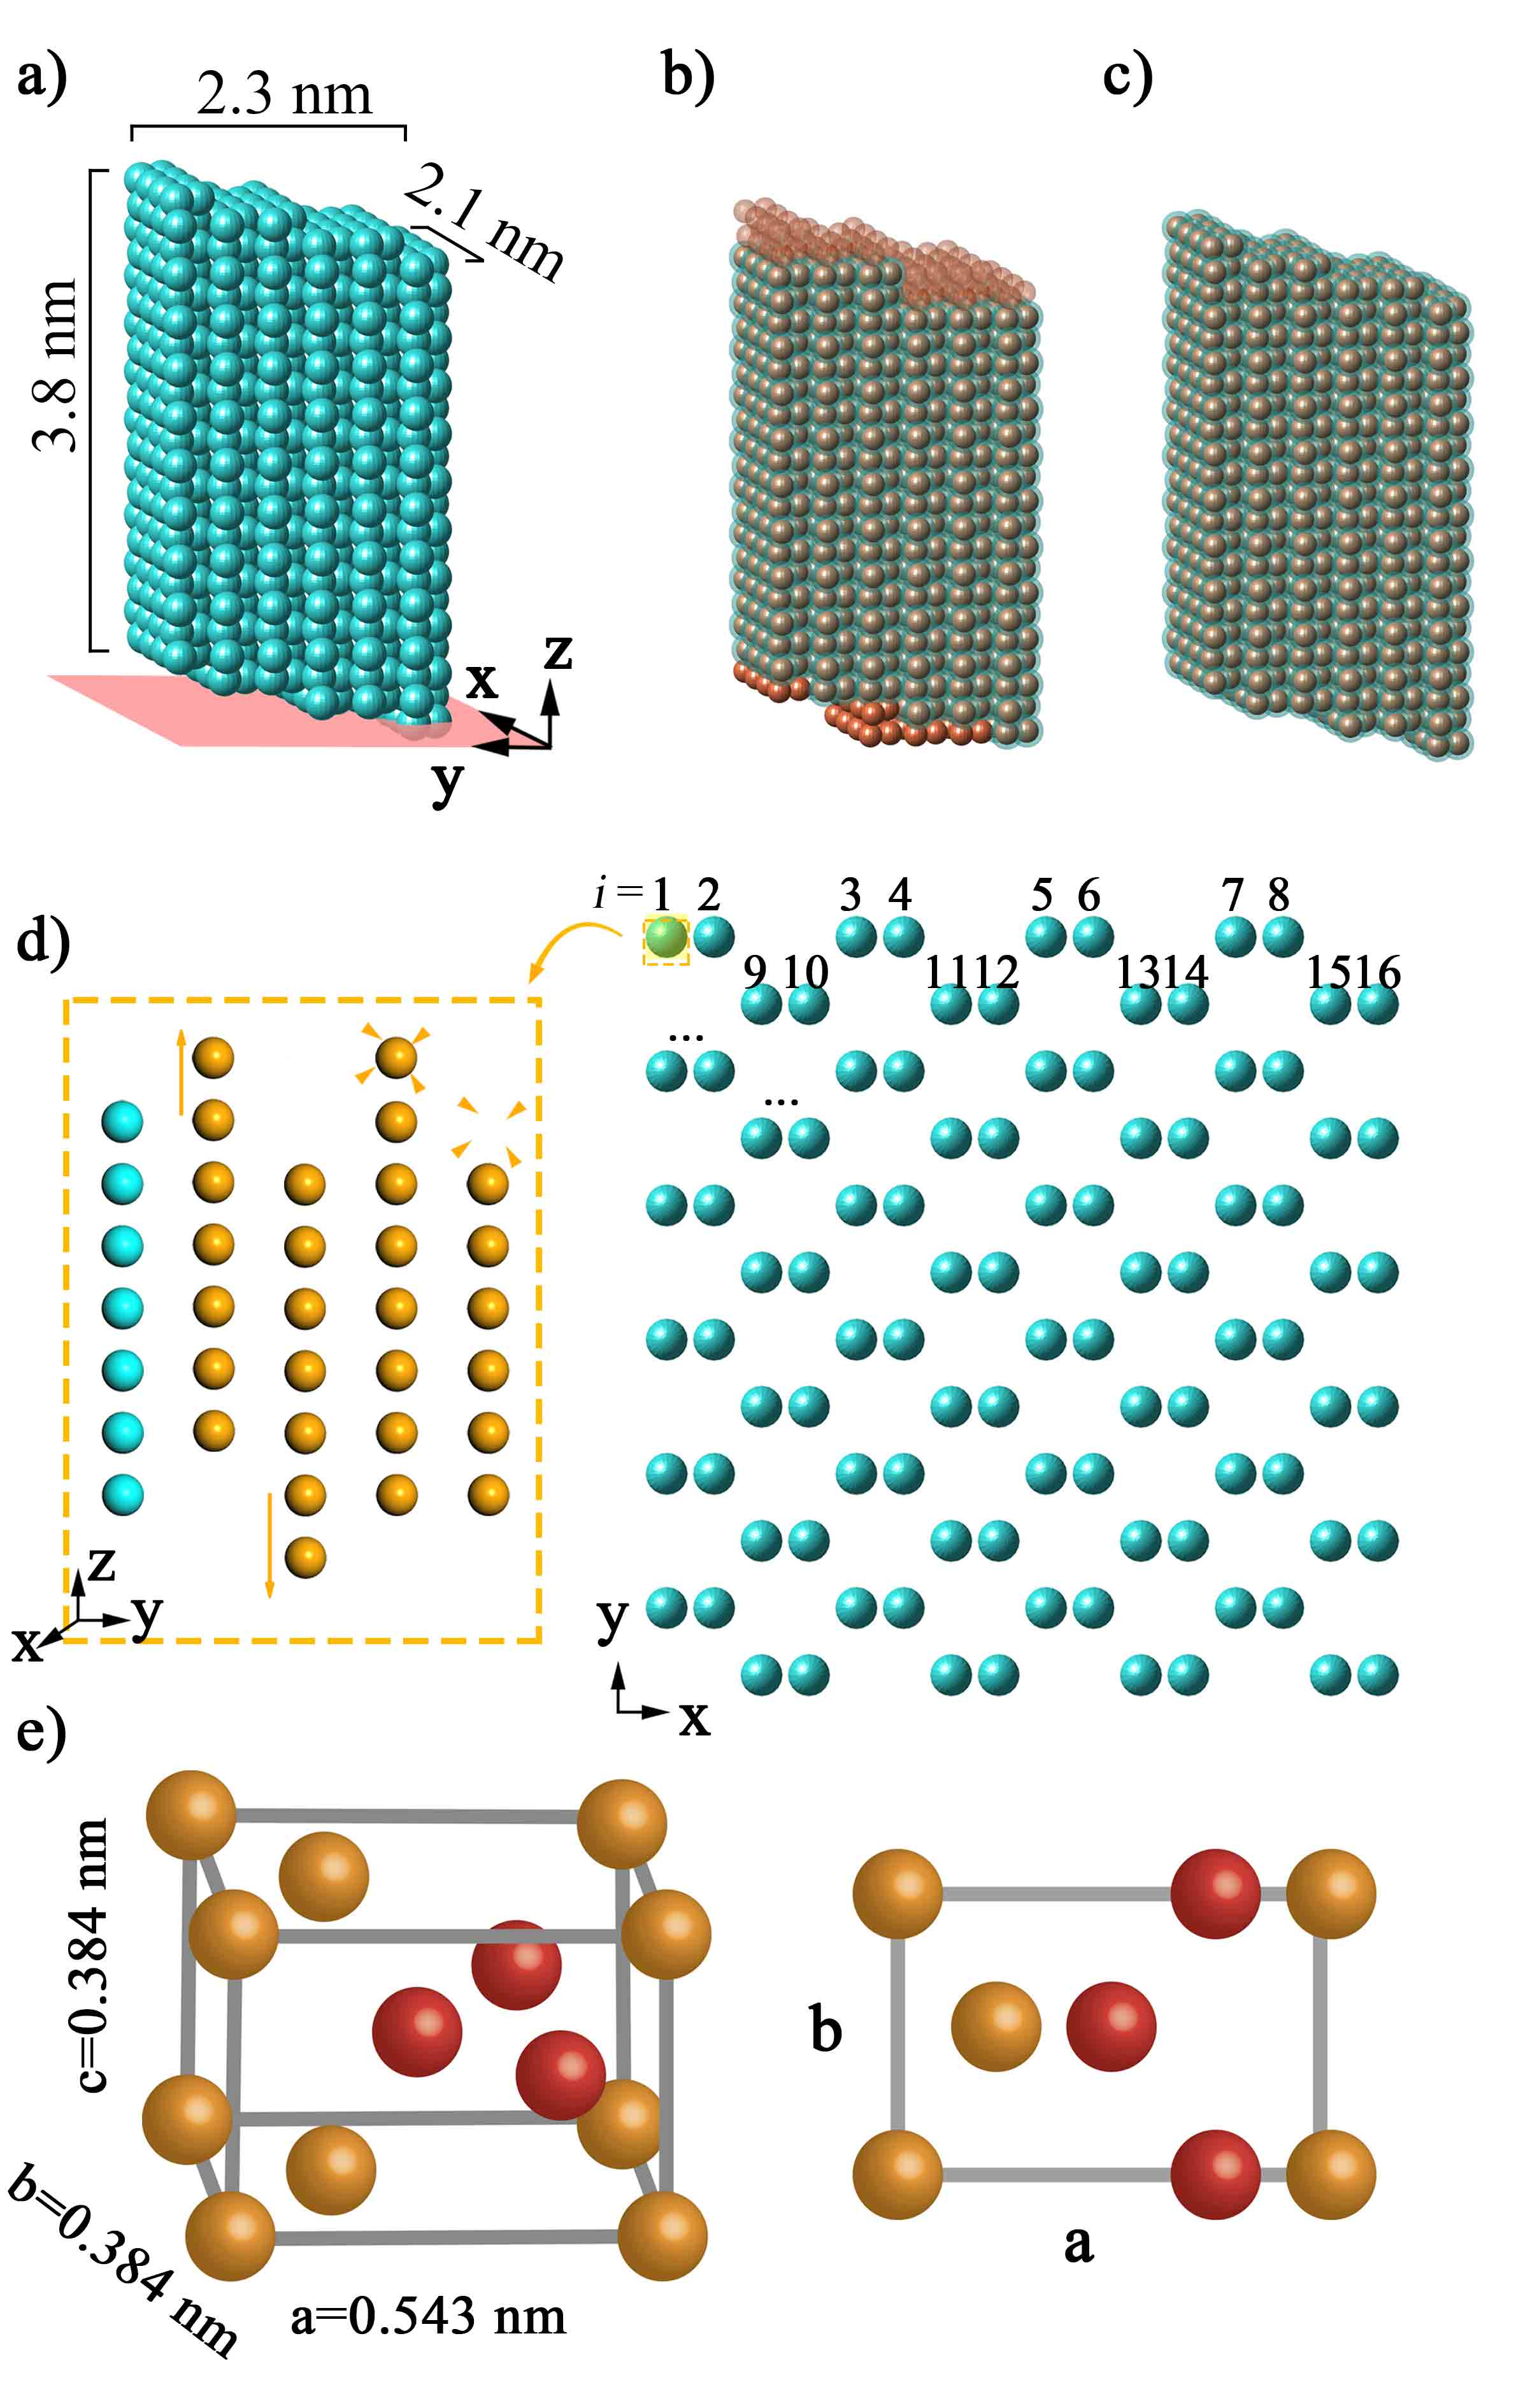
\includegraphics[width=0.8\textwidth]{../2.1/21}
	\caption{模拟测试的示意图}\label{fig:21}
	\song\tuzhu{a) 模拟测试使用的 Si[110] 样品模型的三维形貌图,该模型的上下表面具有一定的倾斜;其中 $x$,$y$,$z$ 轴分别对应 [111],[001],[110] 方向;垂直于 $z$ 轴的粉色平面是零欠焦面;b) 局部匹配算法的重构结果,其表面的一些原子(棕色表示)是错误的,透明棕色表示这些原子没有被正确重构出来;c) 全局匹配算法的重构结果,其与原始模型a)完全一致;d) Si 模型的顶视图,其左边的插图描述了各原子柱在优化时将在厚度(原子柱中的原子个数)和高度(欠焦量)上被调整;每个原子柱在优化时被标记为 $i$ ($i = 1,2, \cdots, N$);e) 左边是 Si[110] 的单胞三维图像,$c$ 平行于 [110];右边是该单胞的顶视图;单胞中橙色的原子处于 $z = 0$ 的位置,而红色的原子处于 $z = 0.5c$ 的位置}
\end{figure}
图 4.1b 是局部匹配算法的重构结果。在这个方法中,整个“实验”图像将以单胞为单位被分割成若干部分。图像的模拟和对比仅分别针对每一个分割出的图像,以确定该图像所对应的原子柱的厚度和欠焦量。从图 4.1b 可知,局部匹配算法所重构的结果相对于原始的结构模型存在明显的误差。尽管如此,它能够合理地反映出原始的原子模型的表面是存在某种程度的倾斜的。图 4.1c 展示了全局匹配算法的重构结果。可以发现,全局匹配算法重构的原子模型与原始模型完全一致,不存在任何误差。

图 4.2 展示了算法的流程图,每当某一 Si 原子柱 $i$($i = 1, 2 \cdots N, N = 96$, 如图 4.1d 所示)发生改变时,整个模型的模拟图像将与实验图像进行对比,对比结果以绝对误差 $D$ 作为评判标准,以优化该原子柱的厚度和高度。所有 $N$ 个 Si 原子柱将被不断地调整优化直到整个模型不再发生任何变化。

\begin{equation}
D=\sum_{i=1}^N \left(\left|I_n-I_n^{exp}\right|\right)/N_{pixel}
\end{equation}

\begin{figure}[htbp]
	\vspace{\baselineskip}
	\centering
	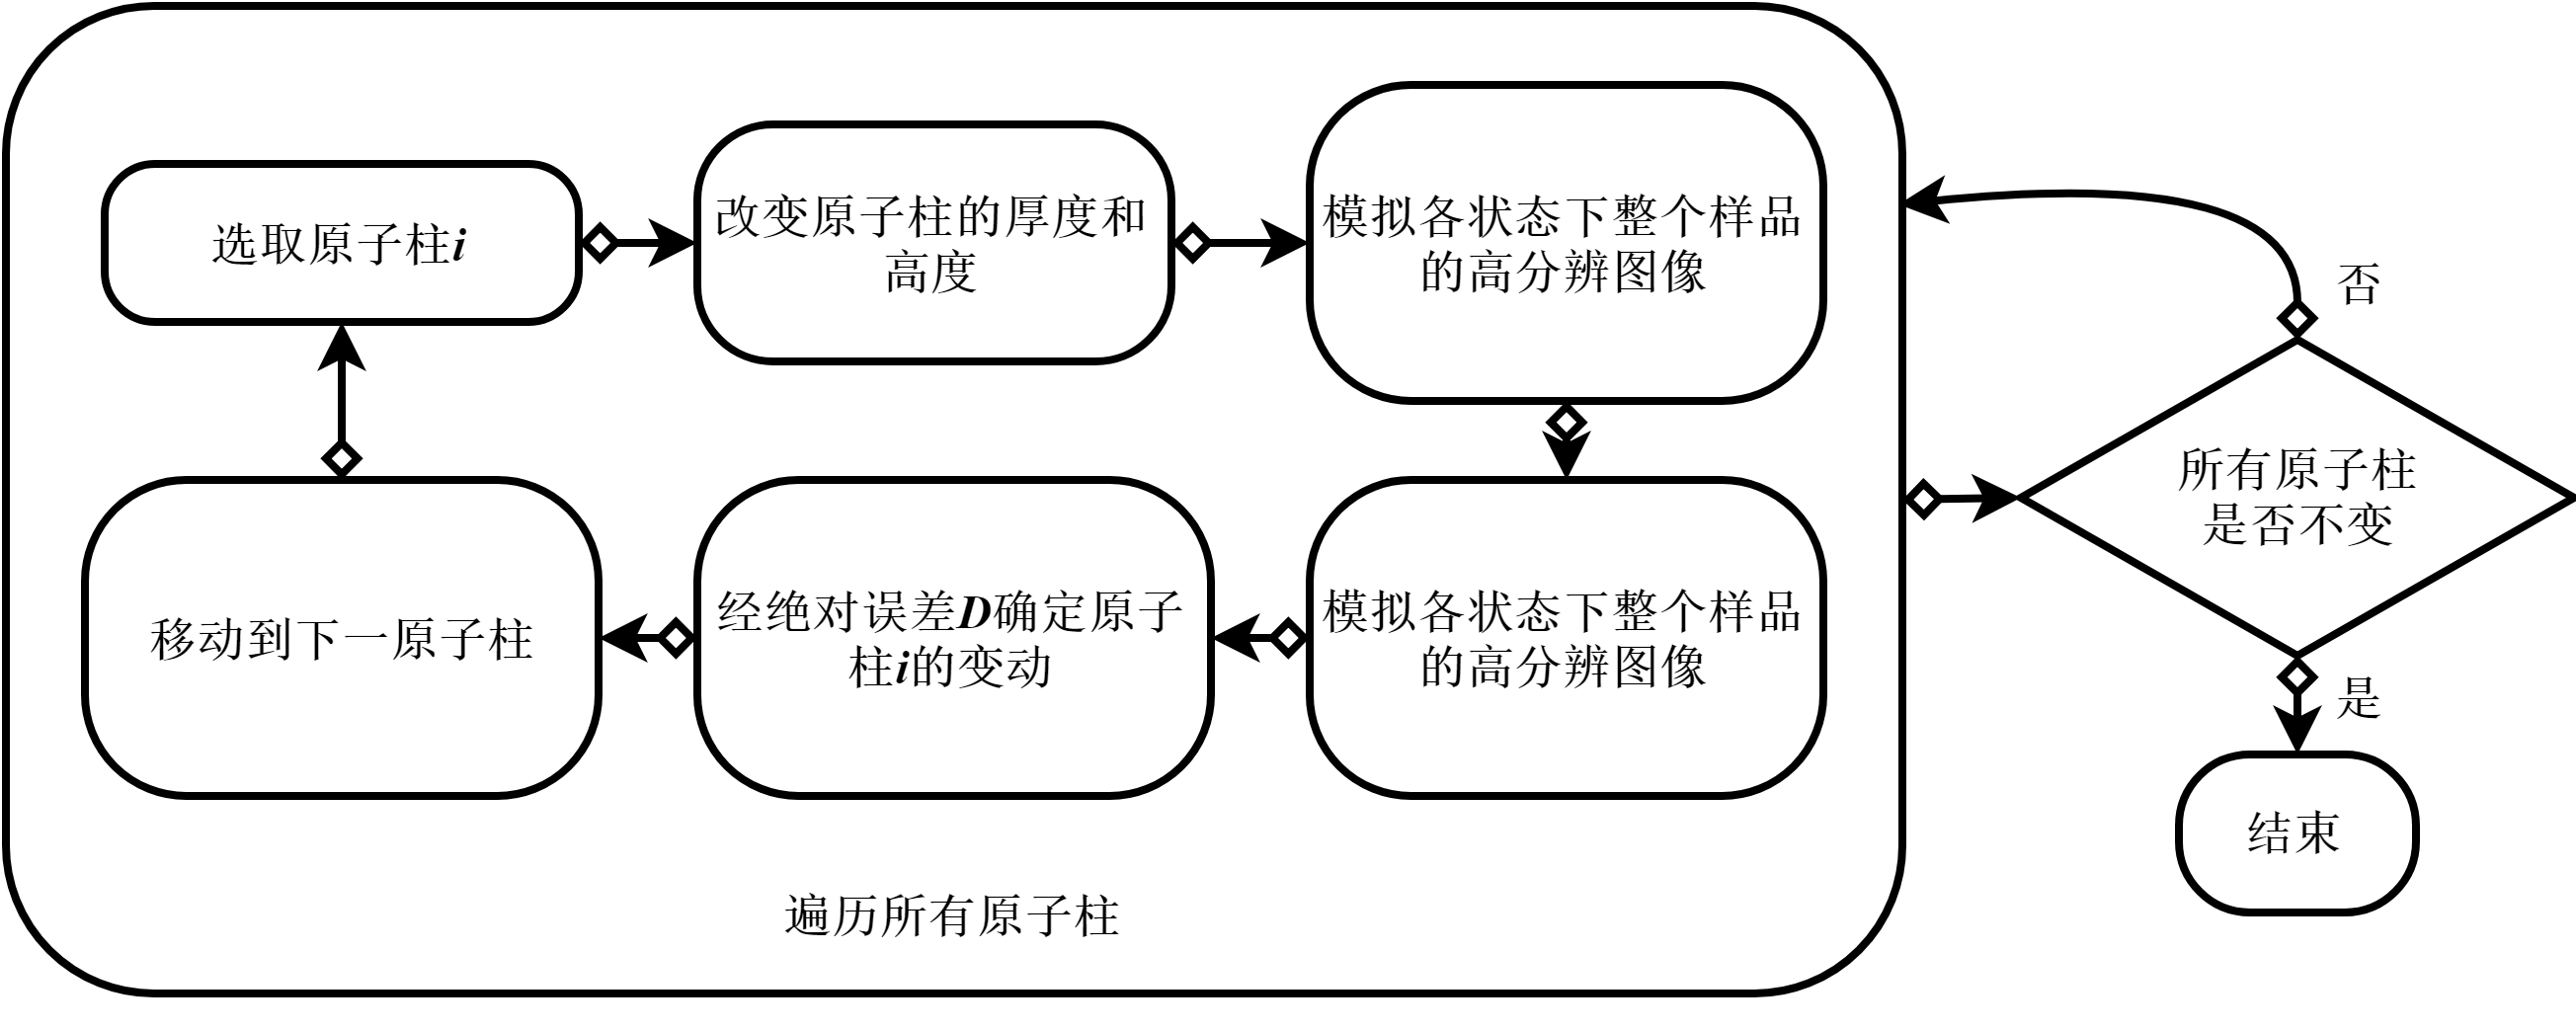
\includegraphics[width=0.8\textwidth]{../2.20/220}
	\caption{算法流程图}\label{fig:220}
\end{figure}

\quad

全局匹配算法的重构结果更加准确的原因主要分为两个方面:首先,全局匹配算法可以避免环绕效应。再者,该方法考虑了包括离域效应在内的所有非线性成像效应。一般来说,由于非线性成像效应,某一原子柱在成像时会影响其周围原子柱的图像衬度。尽管这种效应在原子成像条件下可以被降低到最小,但是不可能被完全消除。因此,在一般的三维重构中,为了达到原子分辨率的重构,应该优先考虑使用全局匹配算法进行重构,而局部匹配算法可以用来重构一个粗略模型为全局匹配算法提供合理的初始模型。

\quad

\begin{table}[htbp]
	\caption{图像模拟参数}\label{tab:table1}
	\vspace{0.5em}\centering\wuhao
	\begin{tabular}{cccc}
		\toprule[1.5pt]
		Parameters & Magnitude\\
		\midrule[1pt]
		Cs$_3$ & 0.015 mm & \\
		Defocus & -3 nm \\
		\quad\quad\quad\quad\quad Semi-Convergence angle\qquad\quad\quad\quad\quad & \quad\quad\quad\quad\quad0.25 mrad\qquad\quad\quad\quad\quad \\
		Objective aperuture & 0.7 $\mathring{A}^{-1}$ \\
		Focus spread & 47 $\mathring{A}$ \\
		Debye-Waller factor & 0.5 $\mathring{A}^2$ \\
		\bottomrule[1.5pt]
	\end{tabular}
	\vspace{\baselineskip}
\end{table}

\subsection{模拟测试方案}
本条将通过重构模拟的高分辨像来测试全局匹配算法。为此构造了如图 4.3a 所示的两个超胞,s1 和 s2。这两个超胞的表面均是倾斜的,这将引起成像的梯度欠焦。且它们的厚度和表面的倾斜程度均不相同,以此作为对比。更详细的超胞信息和模拟参数见图 4.3 和表 4.3。为了避免环绕效应,超胞的左右两端需要加入真空层,并以图 4.3c 中的区域作为重构的感兴趣区域。重构完成后,重构的结果将与正确的超胞进行对比,统计每一个原子柱厚度和高度的误差,并根据公式(4.2)和公式(4.3)计算出平均误差和最大绝对误差:
\begin{equation}
\text{average error} = \sum_{n=1}^N \frac{\left|c_n^{\prime}-c_n\right|}{N}
\end{equation}
其中 $n$ 表示某一原子柱,$N$ 是原子柱的总数,$c_n^{\prime}$ 表示重构的原子柱 $n$ 的厚度或高度,$c_n$ 表示原始超胞中的原子柱 $n$ 的厚度或高度。
\begin{equation}
\text{max absolute error}=\max \left(\left|c_n^{\prime}-c_n\right|\right)
\end{equation}
\begin{figure}[htbp]
	\vspace{\baselineskip}
	\centering
	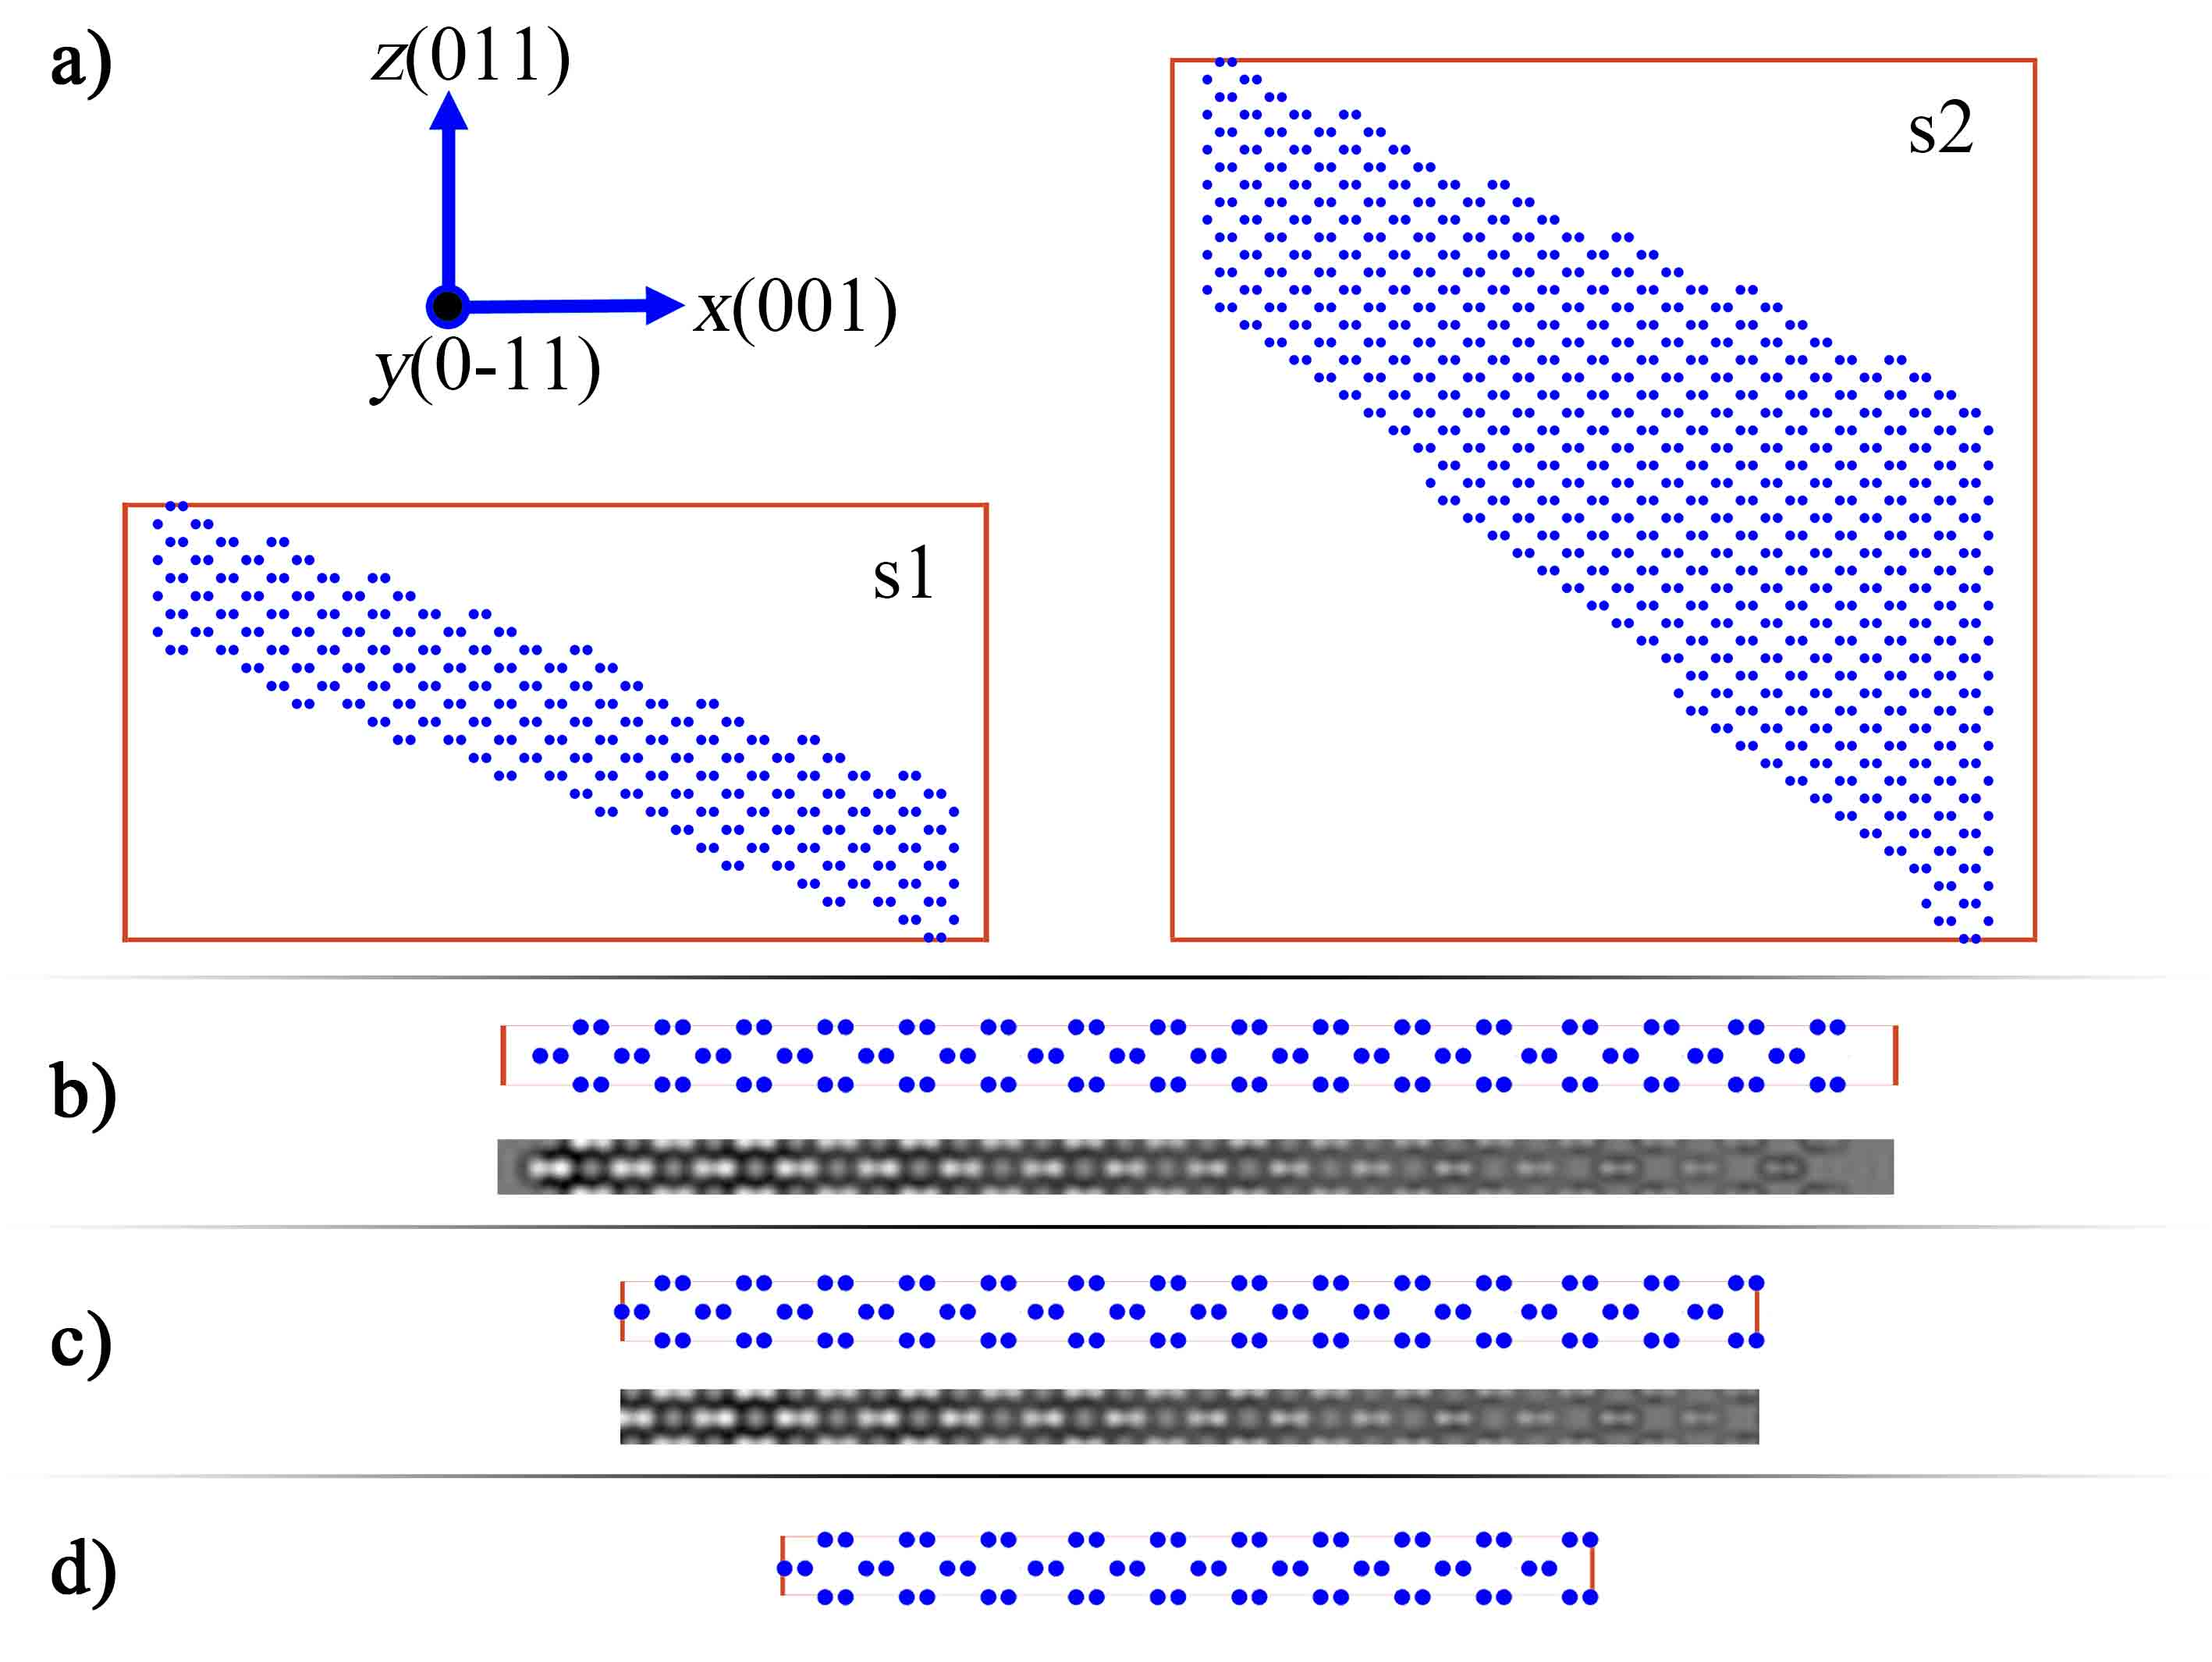
\includegraphics[width=0.9\textwidth]{../2.2/22}
	\caption{超胞 s1 和 s2 的示意图}\label{fig:22}
	\song\tuzhu{a) 超胞 s1 和 s2 的正视图;b) 超胞 s1 和 s2 的俯视图;c) 感兴趣区域的俯视图}
\end{figure}

在模拟测试中,我们讨论了一些重要的参数对全局匹配算法重构的影响,其中包括噪音、欠焦量、晶体倾转、三级球差和 MTF。在实际实验中,这些参数往往无法被精确测定,所以我们还重点探究了这些参数的测量误差对全局匹配算法重构结果的影响。

\begin{table}[htbp]
	\caption{模拟测试中的多层法模拟参数}\label{tab:table1}
	\vspace{0.5em}\centering\wuhao
	\begin{tabular}{cccc}
		\toprule[1.5pt]
		Parameters & Magnitude\\
		\midrule[1pt]
		Side length a & 86.9 $\mathring{A}$ & \\
		Side length b & 3.83 $\mathring{A}$ \\
		\quad\quad\quad\quad\quad Electron beam voltage\qquad\quad\quad\quad\quad & \quad\quad\quad\quad\quad200 kV\qquad\quad\quad\quad\quad \\
		Semi-convergence angle & 0.25 mrad \\
		Objective aperture & 0.7 $\mathring{A}^{-1}$ \\
		Focus spread & 47 $\mathring{A}$ \\
		Debye-Waller factor & 0.5 $\mathring{A}^2$ \\
		Defocus, Cs, crystal tilt, Poisson noise & Zero or specifically defined in tests \\
		\bottomrule[1.5pt]
	\end{tabular}
	\vspace{\baselineskip}
\end{table}

\subsection{模拟测试结果}
\subsubsection{欠焦量、三级球差及晶体倾转对重构的影响}
我们使用全局匹配算法重构了不同欠焦量、三级球差以及晶体倾转下的高分辨 TEM 模拟像以探究这些参数对重构的影响。需要指出的是,在重构中,三级球差和晶体倾转作为已知参数,而欠焦量作为重构的一部分,在重构开始时是未知参数。当 s1 的模拟像中分别加入了 -3 nm 欠焦量、15 $\upmu$m 三级球差或沿 $x-y$ 方向各 15 mrad 晶体倾转后,其重构的结果均如图 4.4a 所示,重构没有误差。同样,当 s2 的模拟像中加入了 -3 nm 欠焦量、15 $\upmu$m 三级球差或沿 $x-y$ 方向 8 mrad 晶体倾转后,其重构结果均如图 4.4b 所示,重构没有误差。然而,当在 s2 的模拟像中加入超过 8 mrad 的晶体倾转时,重构的结果中将产生误差。图 4.4c 是在 s2 的模拟像中加入沿 $x-y$ 方向各 15 mrad 晶体倾转后的重构结果,可见此时重构结果中的误差非常明显。图 4.3d 是在 s2 的模拟像中加入不同程度的晶体倾转产生的误差曲线。可见随着晶体倾转的增加,即使在精确知晓倾转角度时,TEM 像的重构依然将变得越来越困难。

图 4.5a 展示了超胞 s1 和 s2 在欠焦量是 -3 nm 的时候的高分辨 TEM 模拟像。可以看到,图像的衬度随欠焦量的变化发生显著的变化,甚至在某些区域发生了衬度反转的现象(即原子柱的衬度从亮变成了暗)。但即使在这种情况下,全局匹配算法依然可以正确地对其进行重构。图 4.5b 展示了 Si[110] 晶带轴沿 $x$ 方向偏离 8.1 mrad 时的衍射斑点的模拟图像。当晶体倾转为 8.1 mrad 时,电子衍射的偏转已经非常明显。在实际实验操作中,仅通过肉眼观察就能够将晶体倾转控制在 0.4°(约 7 mrad)以内~\cite{Jansen2013}。而且,常规的球差矫正器可以将残余的三级球差控制在 20 $\upmu$m 以内。所以,在球差校正的 TEM 下,经过常规晶带轴校正的 TEM 原子像可以适用于全局匹配算法。以上测试说明了全局匹配算法可以适用于一般的原子分辨率球差矫正 TEM 照片。
\begin{figure}[H]
	\vspace{\baselineskip}
	\centering
	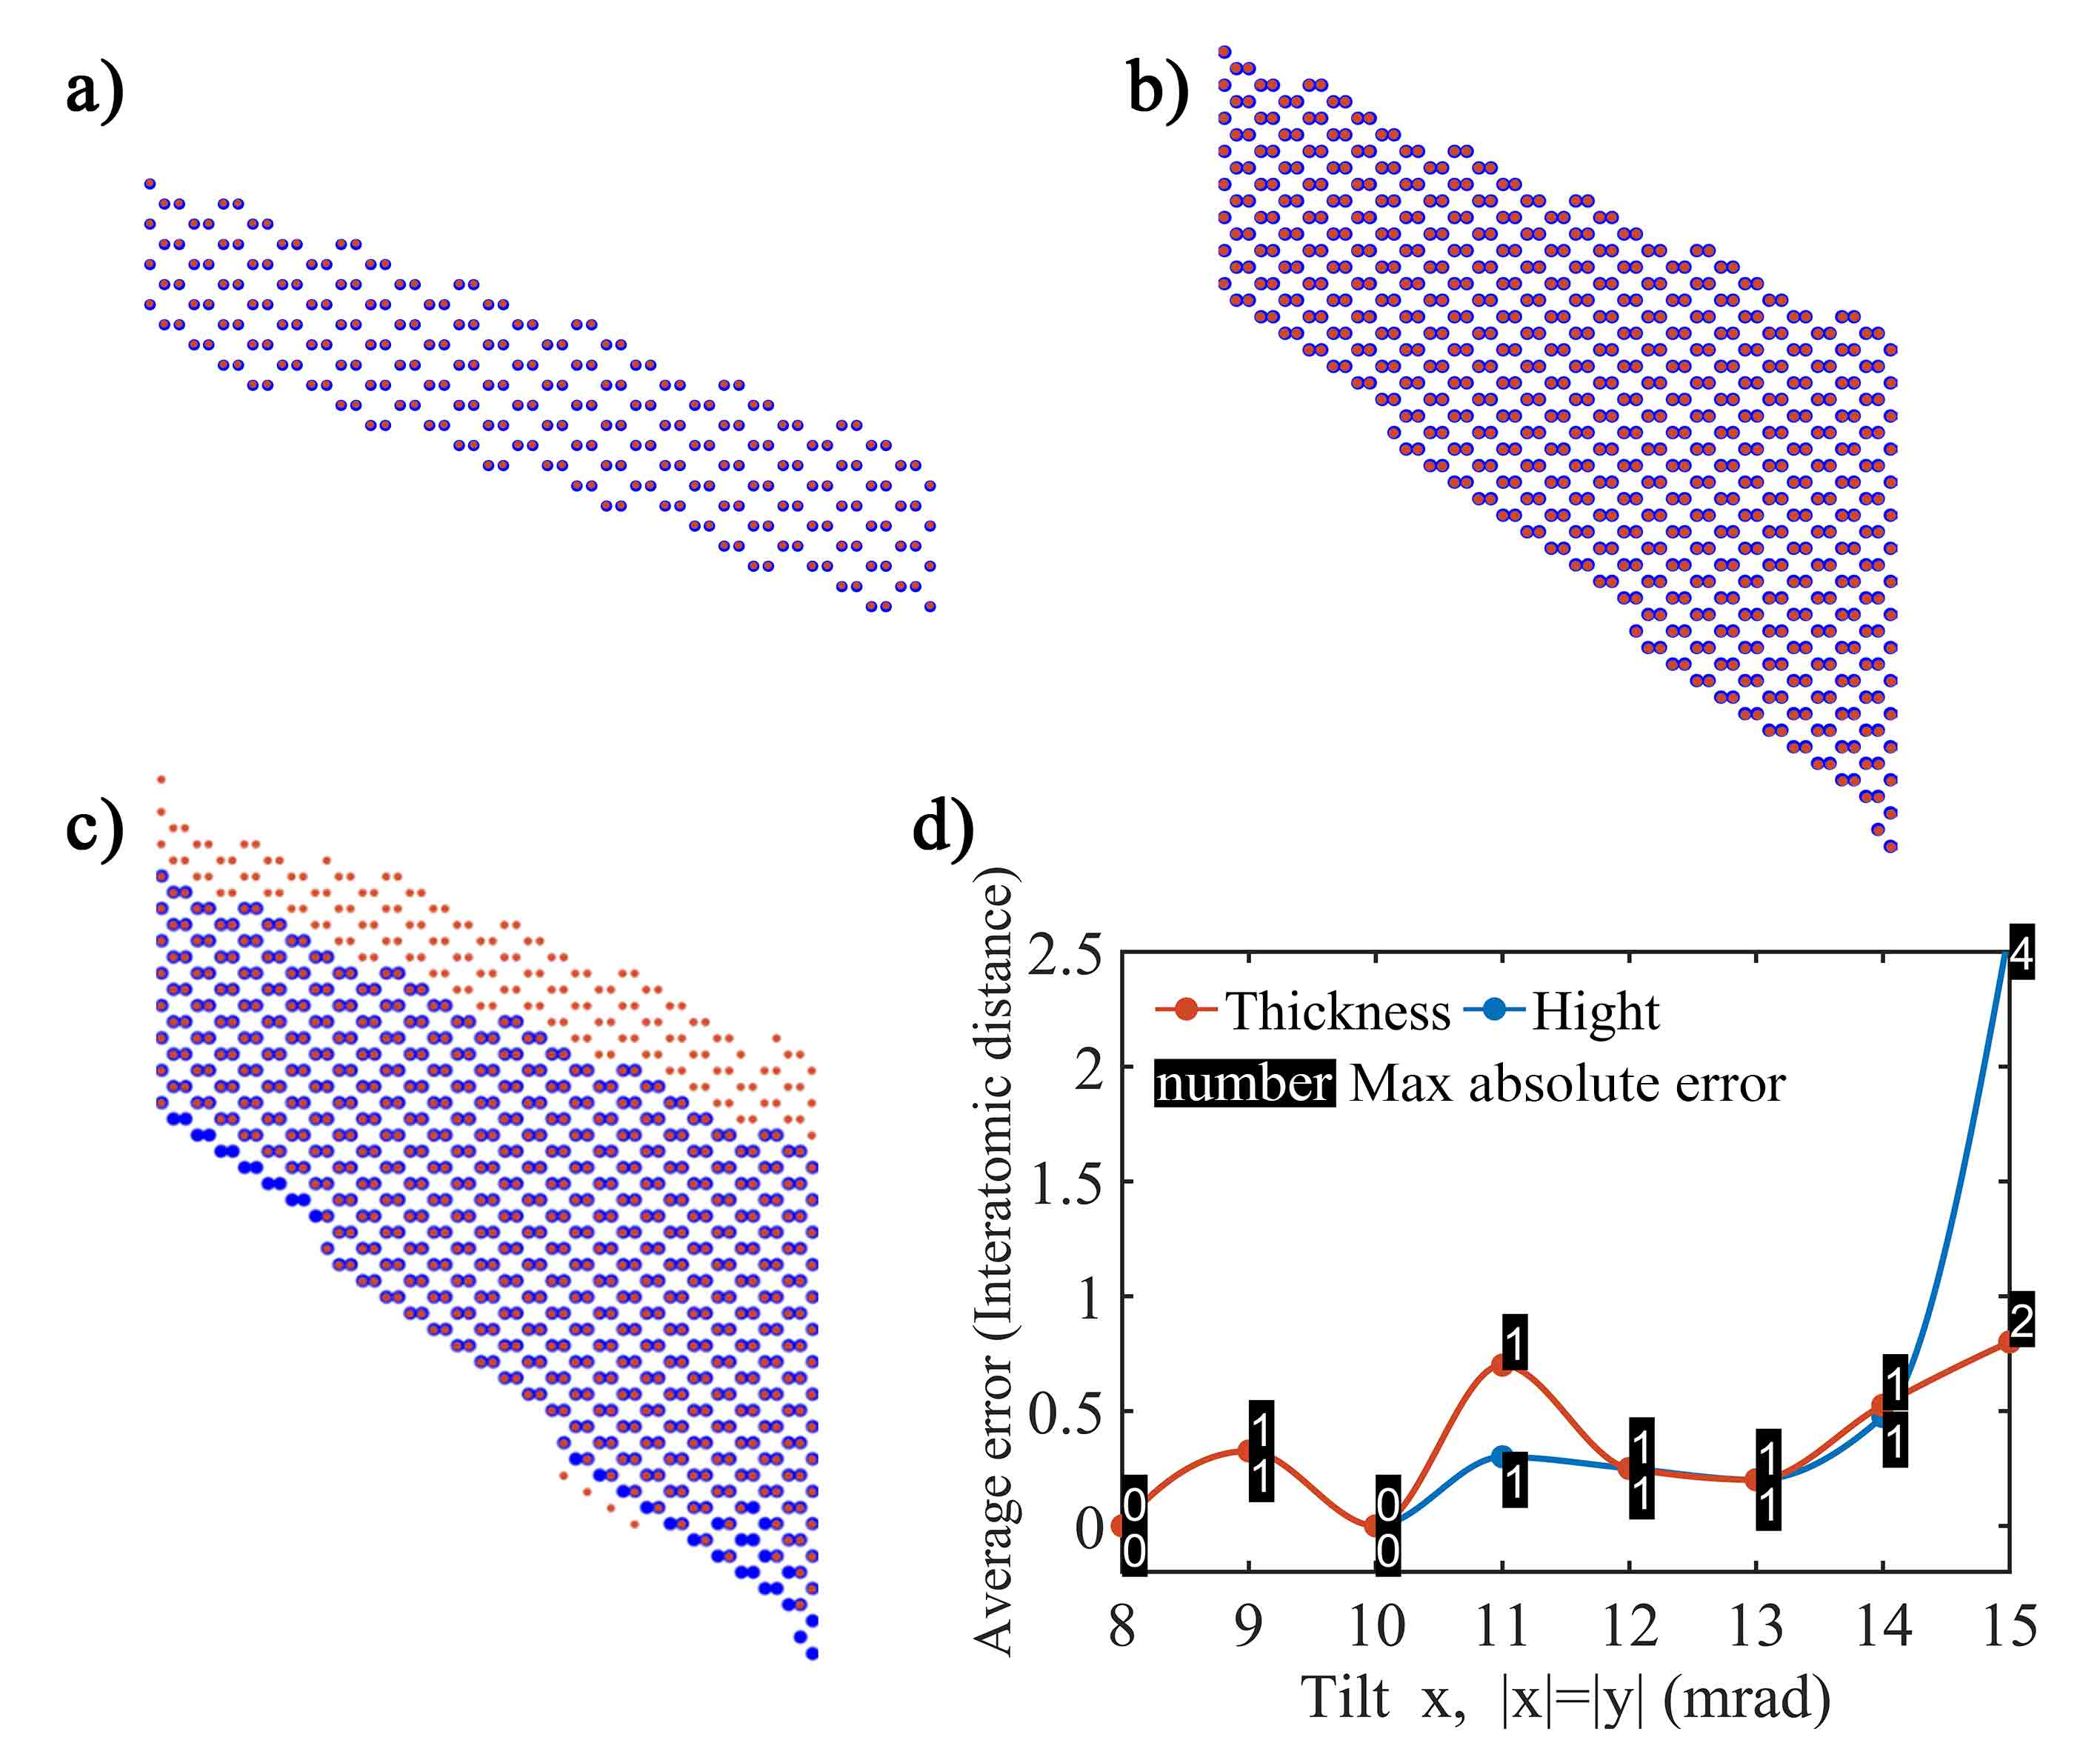
\includegraphics[width=0.75\textwidth]{../2.3/23}
	\caption{模拟测试欠焦量、三级球差、晶体倾转对重构的影响}\label{fig:23}
	\song\tuzhu{a) 当 s1 的模拟像中加入了 -3 nm 欠焦量、15 $\upmu$m 三级球差或沿 $x-y$ 方向各 15 mrad 晶体倾转后的重构结果;b) 当 s2 的模拟像中加入了 -3 nm 欠焦量、15 $\upmu$m 三级球差或沿 $x-y$ 方向各 8 mrad 晶体倾转后的重构结果;c) 当 s2 的模拟像中加入了沿 $x-y$ 方向各 15 mrad 晶体倾转后的重构结果;图 a-c 中背景蓝色原子模型是原始的超胞模型,欠焦红色原子模型是重构结果;d) 当 s2 的模拟像中加入不同程度的晶体倾转后的重构结果的误差变化曲线}
\end{figure}
\begin{figure}[H]
	\vspace{\baselineskip}
	\centering
	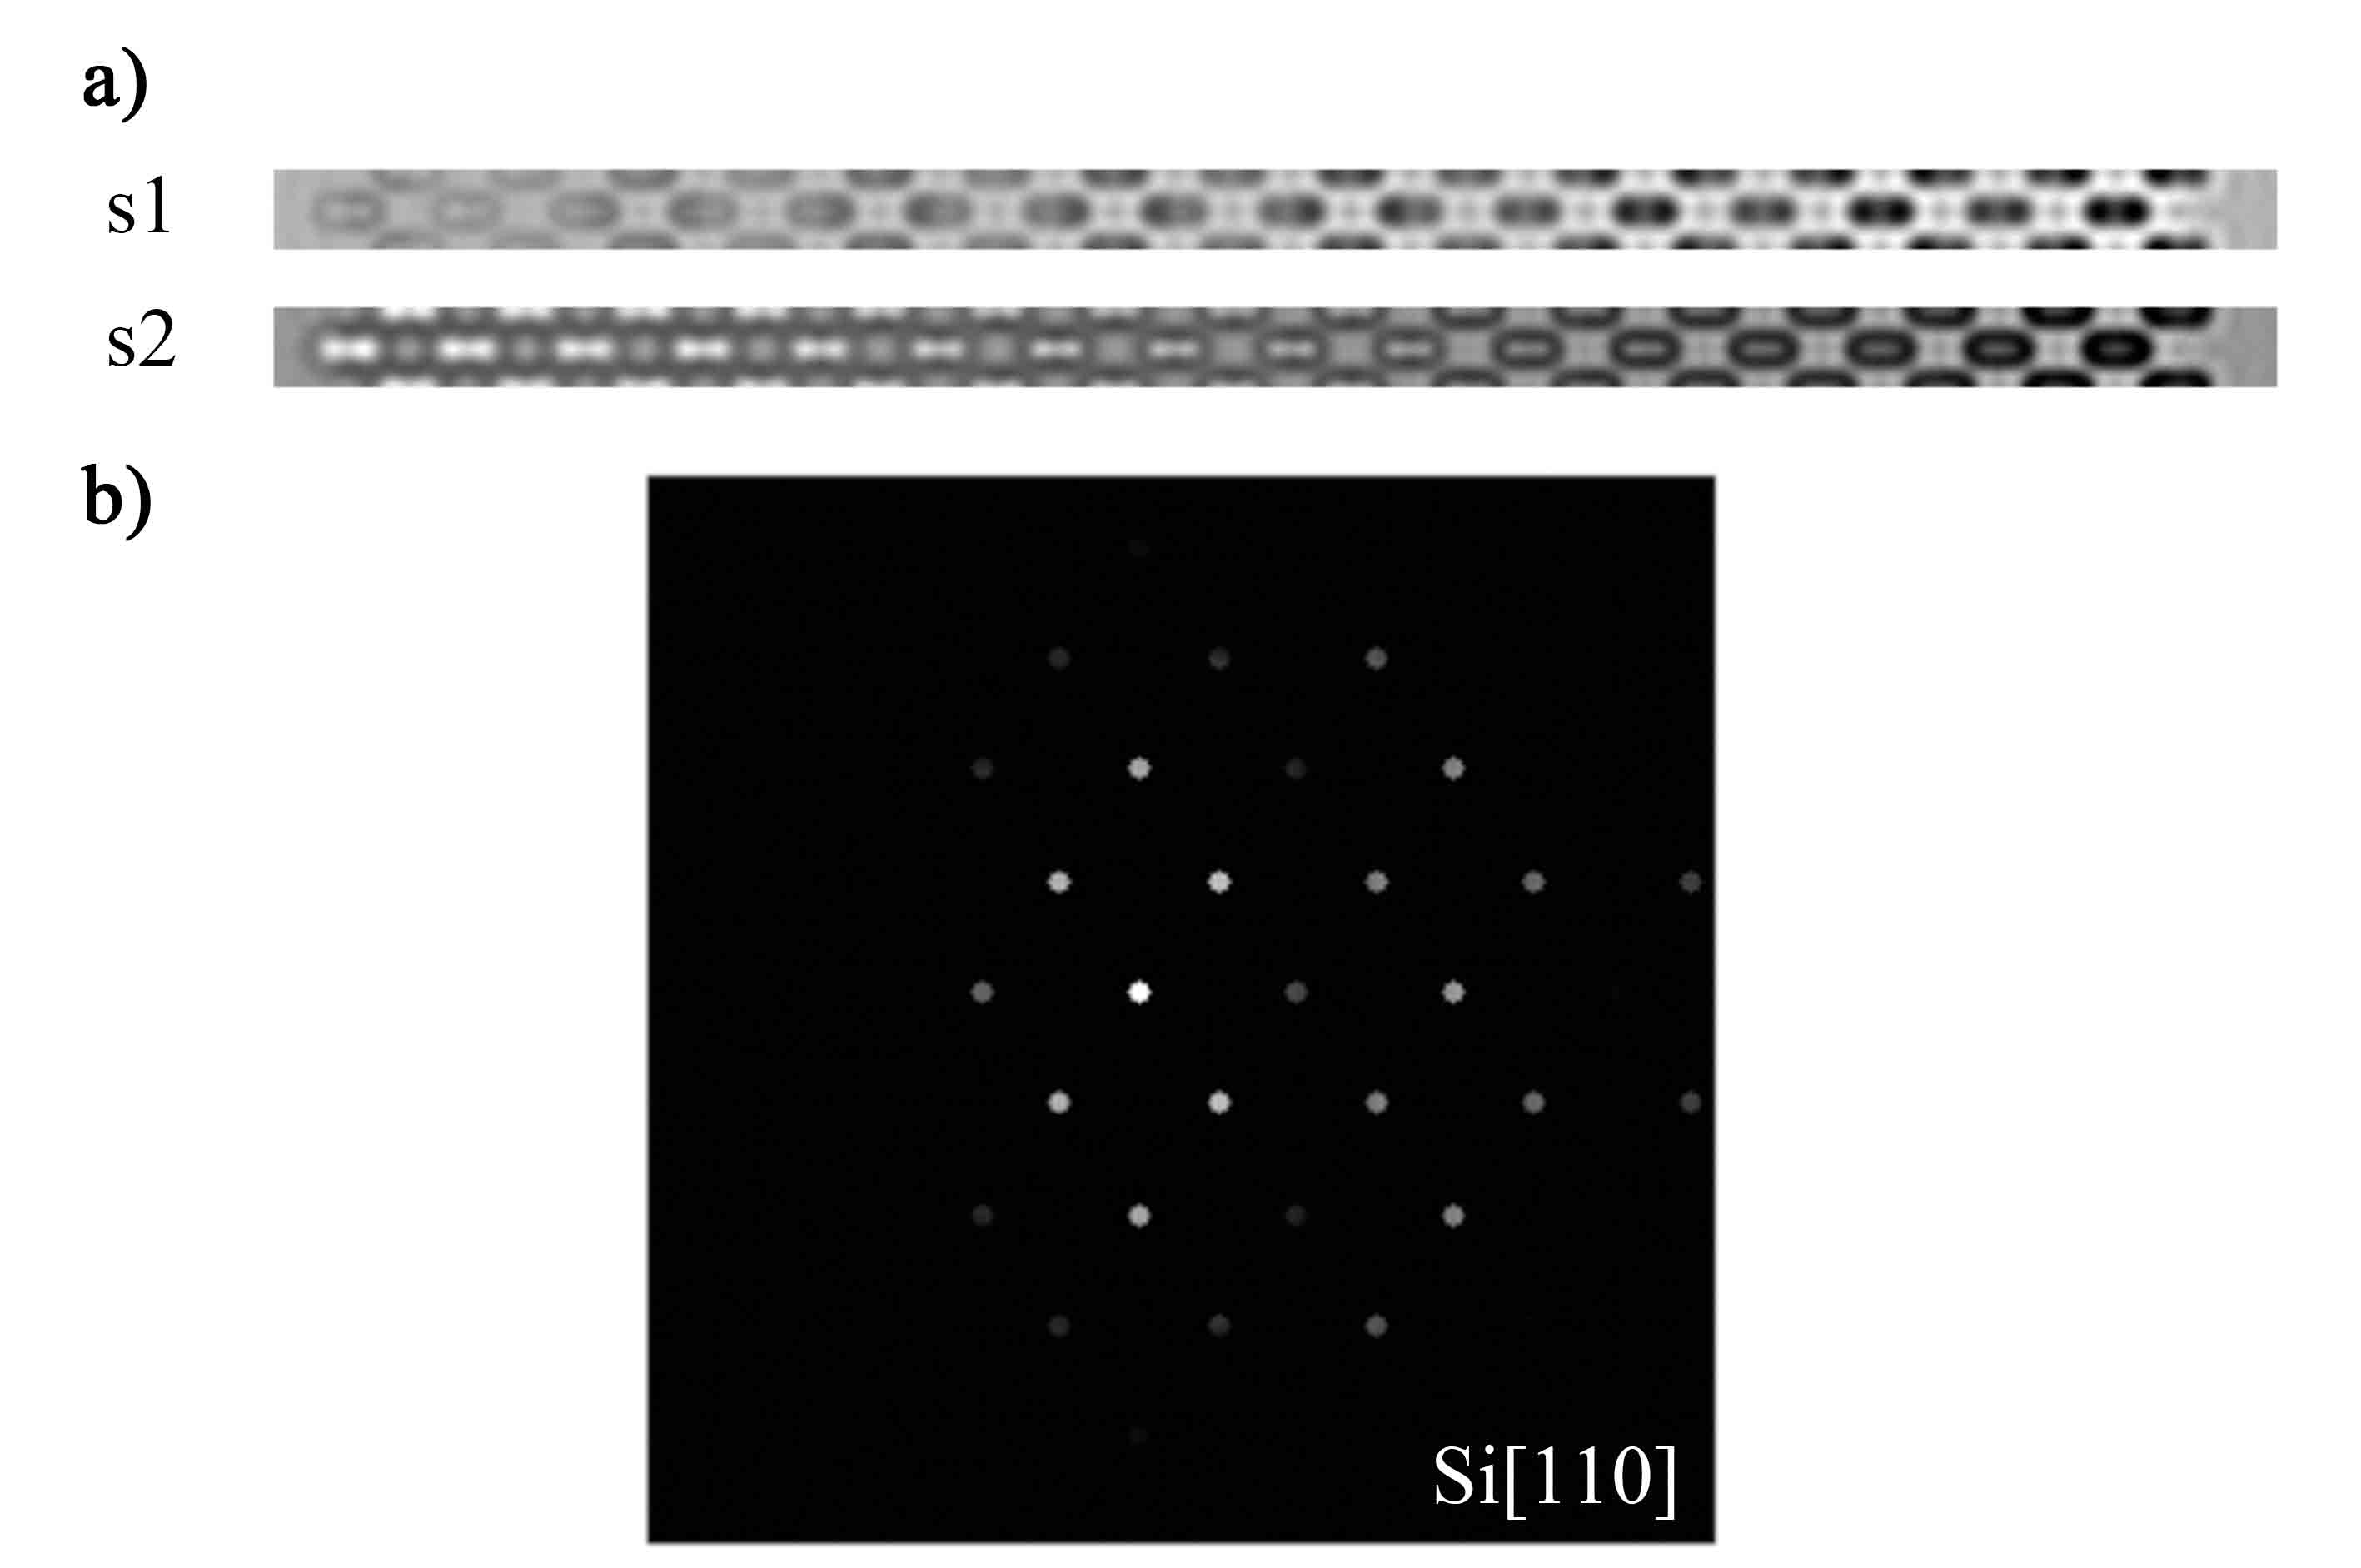
\includegraphics[width=0.75\textwidth]{../2.4/24}
	\caption{超胞 s1 和 s2 在 -3 nm 欠焦量下的模拟像及 Si[110] 在 8.1 mrad 晶体倾转下的电子衍射模拟图}\label{fig:24}
	\song\tuzhu{a) s1 和 s2 在 -3 nm 欠焦量下的模拟像;b) Si[110]晶体在沿 $x$ 方向倾转 8.1 mrad 时的电子衍射模拟图}
\end{figure}

\subsubsection{噪音对重构的影响}

噪音在实验中是不可避免的,它会降低成像质量,影响图像定量分析。为了探究在噪音的存在下,全局匹配算法是否依然能够对图像进行精确重构,我们将泊松噪音加入到了模拟像中,再用全局匹配算法对其进行重构。图 4.6a 和 b 分别展示了当在 s1 和 s2 的模拟像中加入不同信噪比的泊松噪音时的误差变化曲线。可以看到,当信噪比增加到 30 db 时,重构误差几乎消失,当信噪比逐渐降低时,重构误差也将增加。图 4.6c 和 d 展示了加入 30 db 泊松噪音的 s1 和 s2 的部分模拟像。尽管加入的噪音的信噪比相同,但是图 4.6c 和 4.6d 图像质量的下降程度是不同的,这主要是因为 s2 比 s1 厚,所以其 TEM 照片的衬度比 s1 的高,不容易被噪音影响。不过,尽管 s1 的图像质量受噪音的影响如此严重,此时产生的重构误差却很小。所以噪音不会对全局匹配算法产生特别明显的影响。

\begin{figure}[htbp]
	\vspace{\baselineskip}
	\centering
	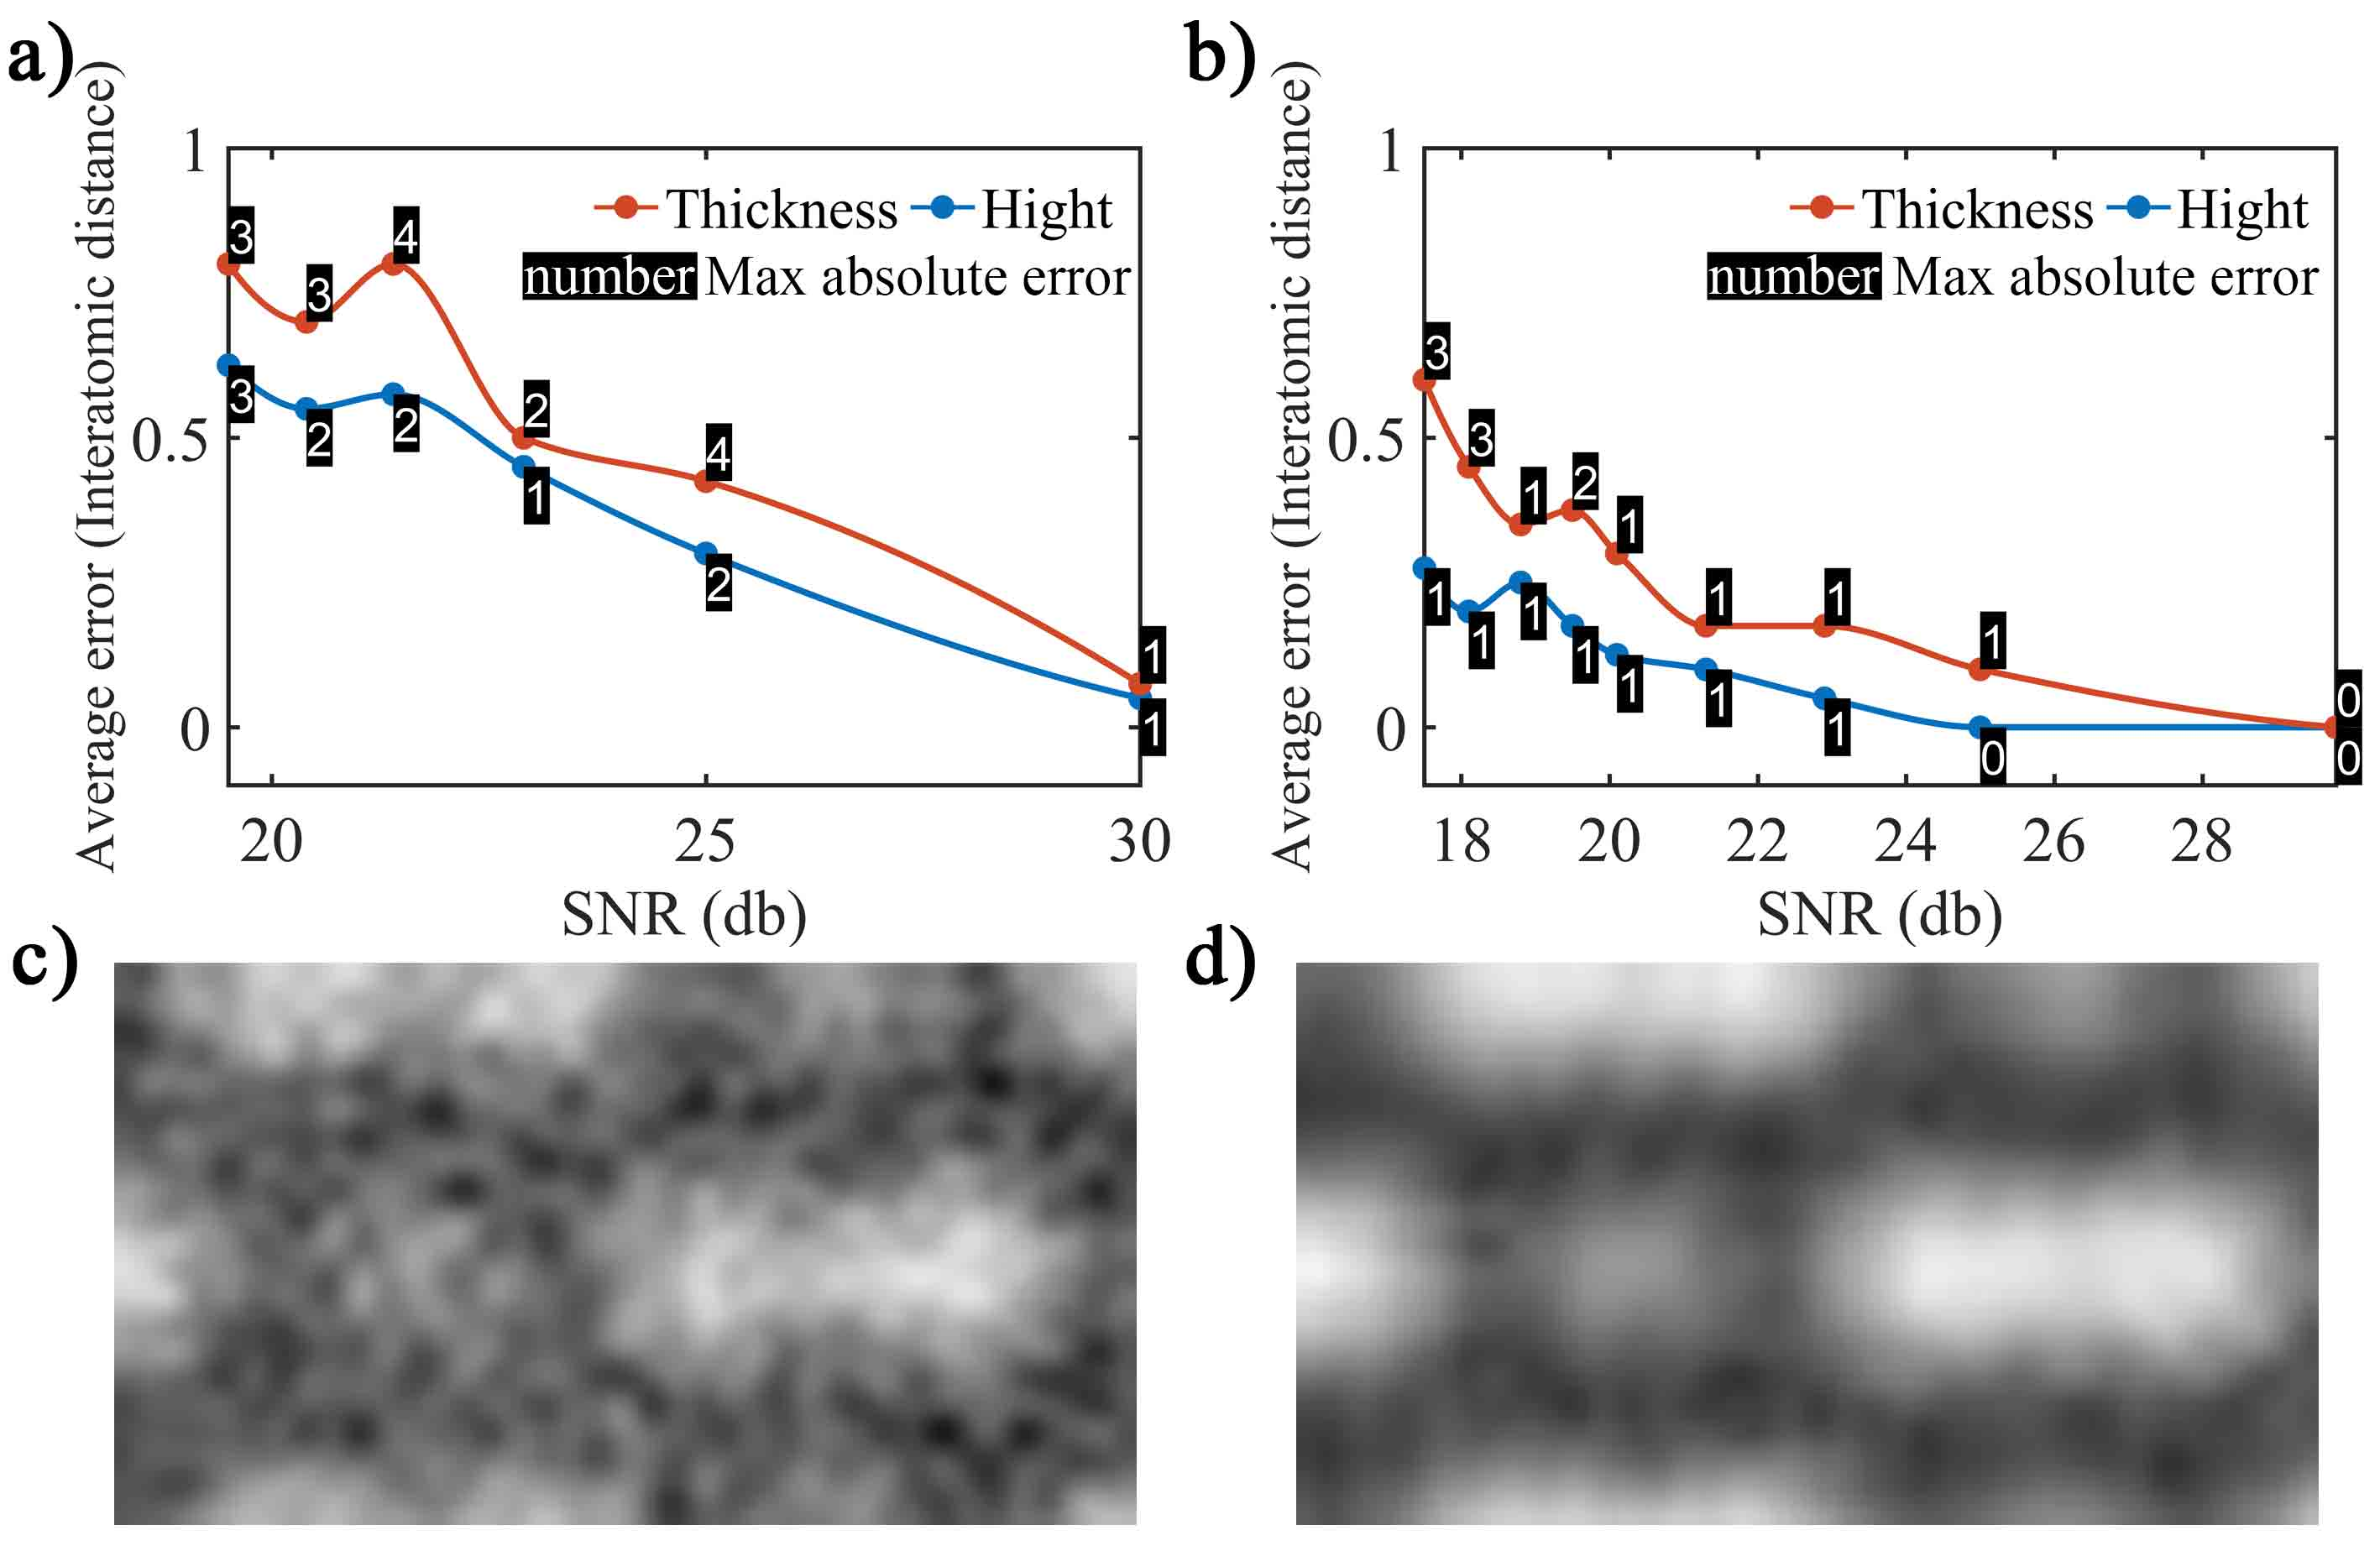
\includegraphics[width=0.9\textwidth]{../2.5/25}
	\caption{模拟测试噪音对重构的影响}\label{fig:25}
	\song\tuzhu{a,b) s1 和 s2 的重构误差关于噪音信噪比的变化曲线;c,d) 加入了 30 db 的泊松噪音后的 s1 和 s2 的部分模拟像}
\end{figure}

\subsubsection{晶体倾转测量误差对重构的影响}
在 TEM 中观察晶体的高分辨图像时,需要倾转晶体使其晶带轴与电子束入射方向平行。在实际操作中,往往无法保证完美地将晶带轴踩正,而残余的晶体倾转又很难被准确地测量。本节通过模拟讨论无法准确知晓晶体倾转的时候是否还能进行精确的三维重构。为此我们首先在 s1 的模拟像中加入了沿 $x$ 和 $y$ 方向各 15 mrad 的晶体倾转,在 s2 的模拟像中加入了沿 $x$ 和 $y$ 方向各 8 mrad 的晶体倾转(在第 4.2.3.1 款 中已经证明,当精确已知晶体倾转时,这两个模型都能被精确重构)。然后,在重构模拟像时使用不同程度的晶体倾转以观察重构结果的变化情况。图 4.7a 和 b 展示了以不同晶体倾转重构 s1 和 s2 时的误差变化曲线。当使用的晶体倾转偏离正确数值时,重构误差逐渐增加。由于 s2 超胞比 s1 厚,所以其高分辨像的衬度变化更易受晶体倾转的影响,在相同的晶体倾转数值偏离下,其产生的重构误差也更大。不过,当晶体倾转的误差保持在几个毫弧度内时,其导致的重构误差在一个单胞长度以内。在 s1 中,晶体倾转的数值偏离引起的重构误差更小,在一定程度内几乎可以被忽略。所以,晶体倾转的测量误差对厚样品的重构具有一定的影响。不过,厚样品的图像衬度受晶体倾转的影响较大,在实际使用时只要保证使用高质量的 TEM 像就可以避免过大的晶体倾转带来的误差。
\begin{figure}[htbp]
	\vspace{\baselineskip}
	\centering
	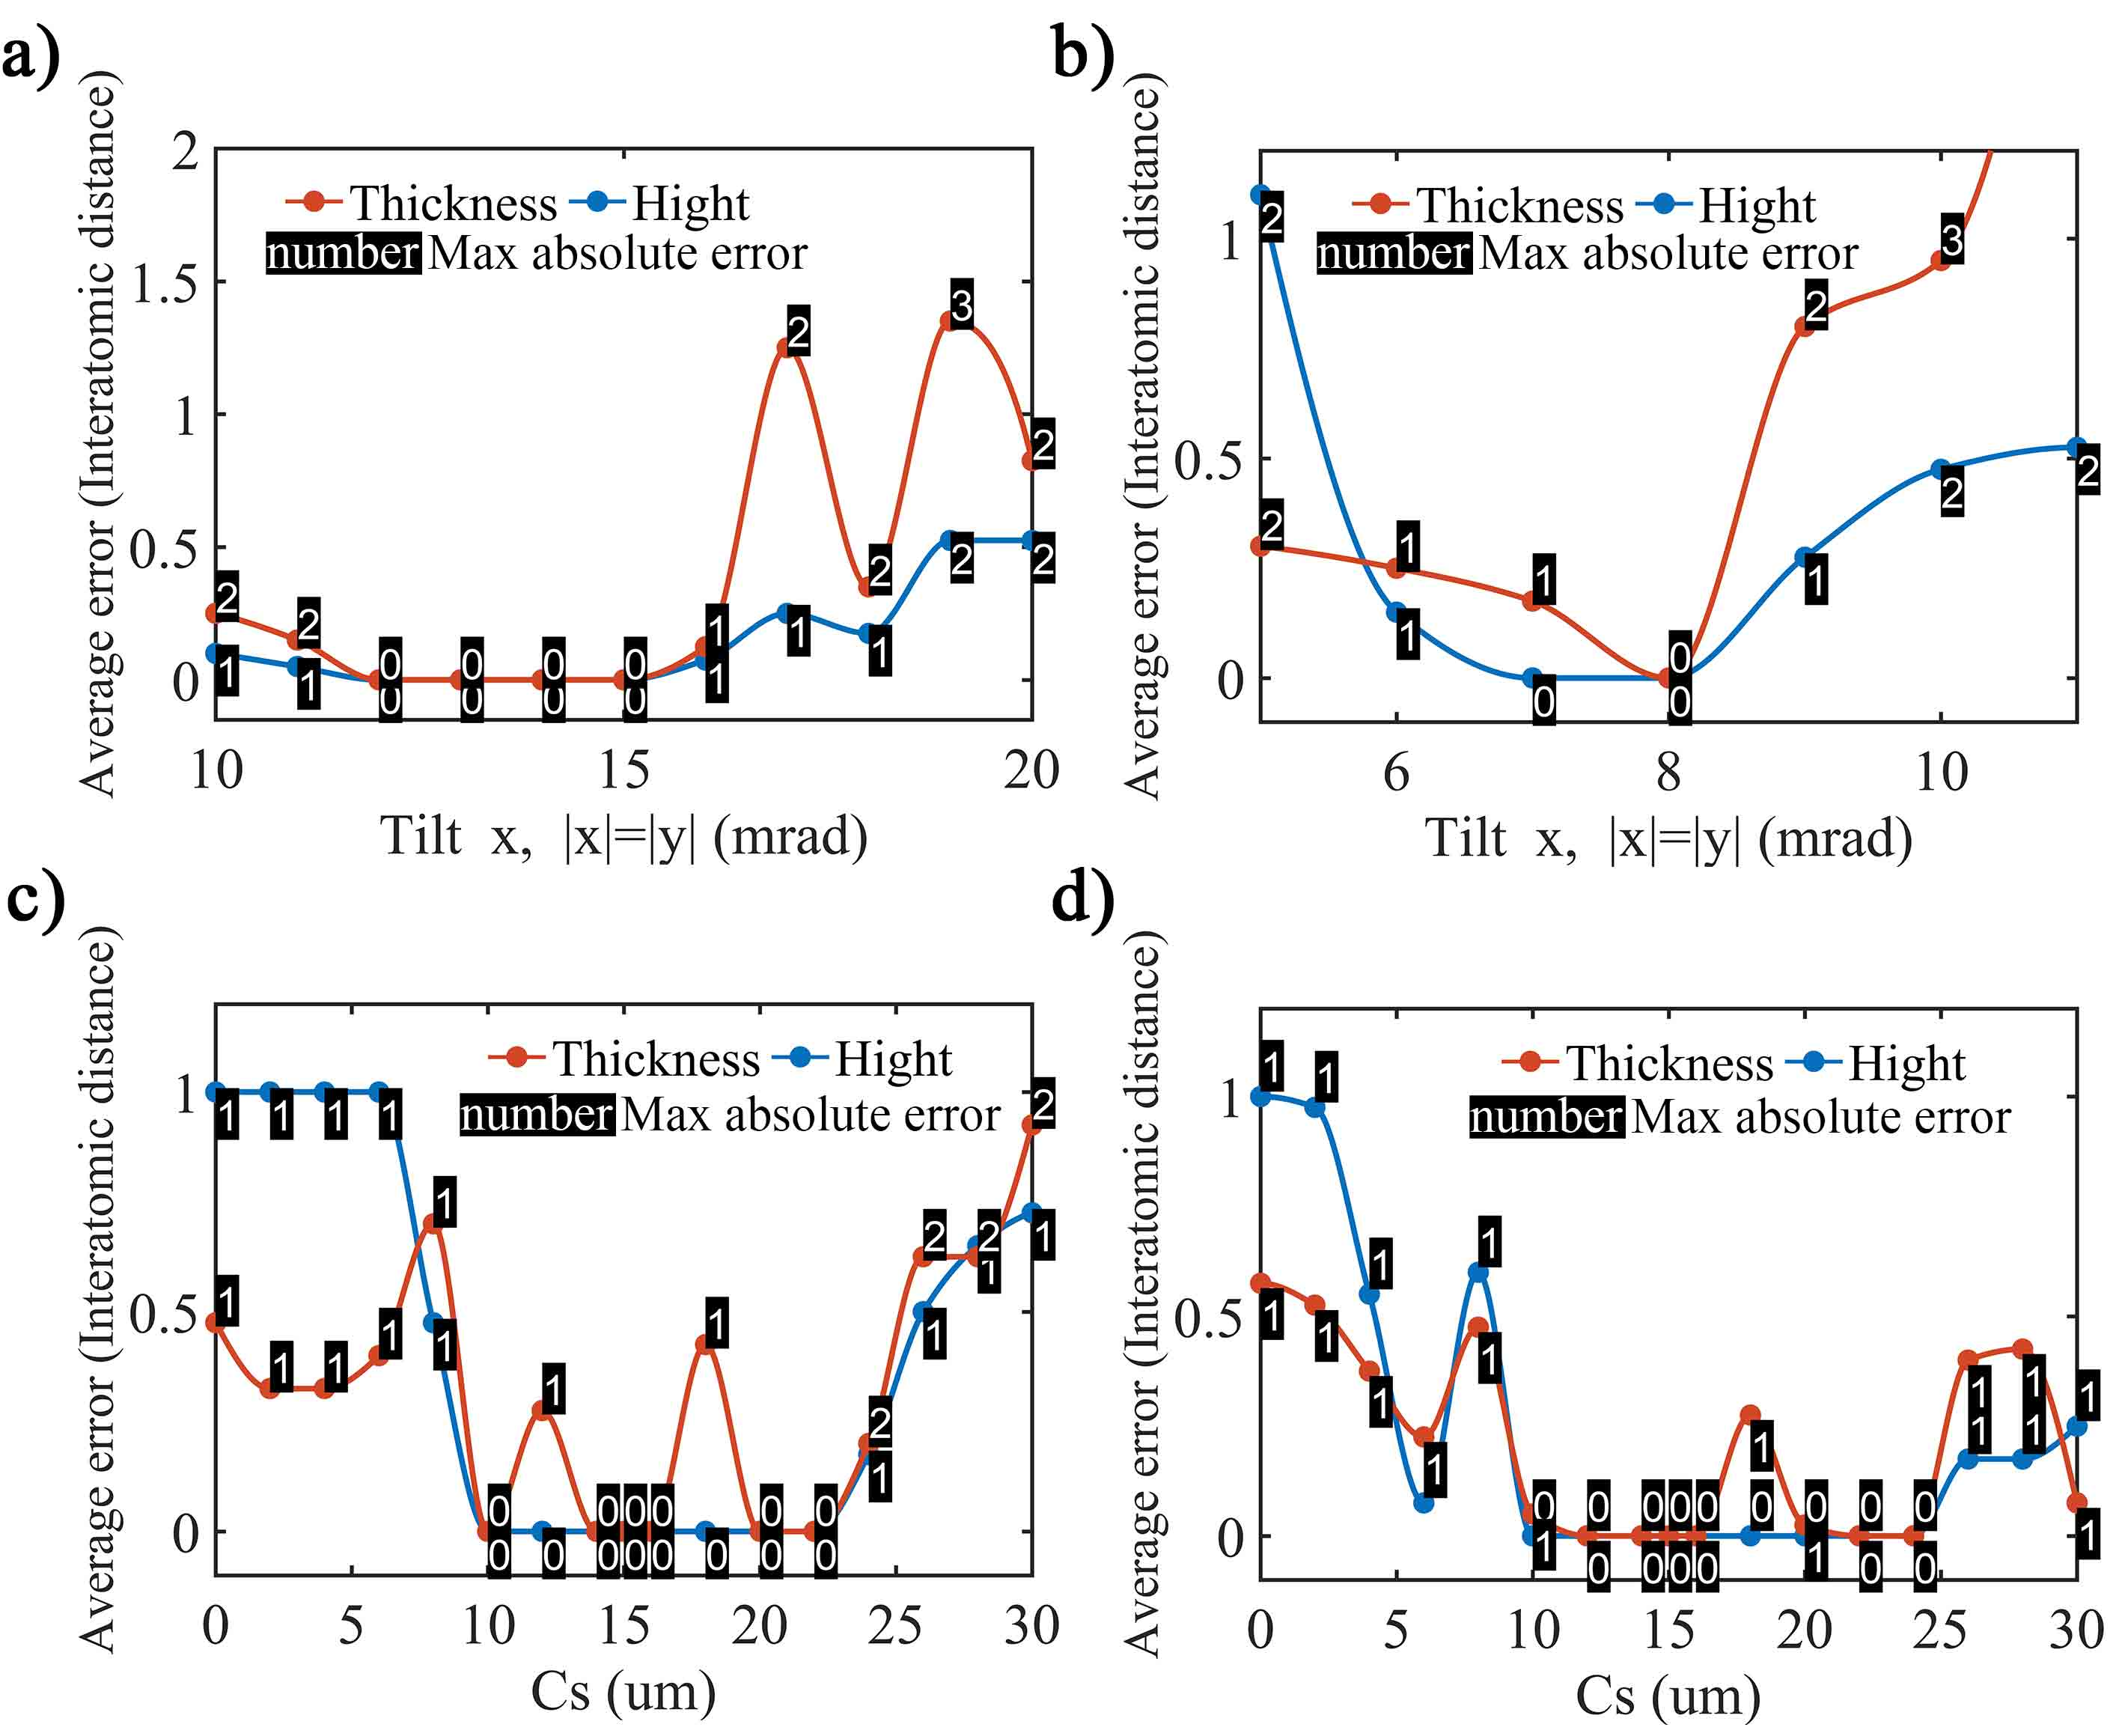
\includegraphics[width=0.9\textwidth]{../2.6/26}
	\caption{模拟测试晶体倾转以及三级球差测量误差对重构的影响}\label{fig:26}
	\song\tuzhu{a) 以不同程度的晶体倾转重构含 15 mrad 晶体倾转的 s1 模拟像时的误差变化曲线;b) 以不同程度的晶体倾转重构含 8 mrad 晶体倾转的 s2 模拟像时的误差变化曲线;c) 以不同程度的三级球差重构含 15 $\upmu$m 三级球差的 s1 模拟像时的误差变化曲线;d) 以不同程度的三级球差重构含 15 $\upmu$m 三级球差的 s2 模拟像时的误差变化曲线}
\end{figure}

\subsubsection{三级球差测量误差对重构的影响}
三级球差(third order spherical aberration,Cs)是 TEM 成像过程中非常重要的像差参数,在球差矫正器发明之前,它一直是限制 TEM 分辨率的重要因素。在实际的实验中,尽管球差矫正器能够将三级球差矫正到很小量级,但是其测量到的球差与真实的球差之间总可能存在误差。当无法准确知道真实球差的数值时,是否还能进行精确的三维重构是一个需要被探究的问题。本节在 s1 和 s2 的模拟像中都加入了 15 $\upmu$m 的三级球差,并在重构时,使用不同数值的三级球差。图 4.7c 和 d 是以不同的三级球差重构 s1 和 s2 时的重构误差变化曲线。当三级球差的测量误差在 $\pm$5 $\upmu$m 以内,重构的平均误差将保持在 0.4 个单胞长度以内,且最大误差不超过 1 个单胞长度,这说明重构的结果中只有少数原子柱产生一个单胞长度的重构误差。总体而言,三级球差对重构结果的影响不大,即使存在一定的常规测量误差,也可以进行准确的三维重构。

\subsubsection{MTF 矫正误差对重构的影响}

在电镜中,CCD 相机收集到的图像强度与理论上的图像强度是不一致的,MTF 函数描述了两者之间的关系。公式(4.4)是公式(1.23)简化 $MTF_{px}$ 和 $C$ 之后的结果:
\begin{equation}
H=F \cdot \textit{MTF}_{px}
\end{equation}
其中 $H$ 表示 $CCD$ 相机收集到的 TEM 照片的傅里叶变换,$F$ 表示理想的 TEM 照片的傅里叶变换,$\textit{MTF}_{px}$ 如下式所示~\cite{VanBroek2012}:
\begin{equation}
\textit{MTF}_{px}(u,v)=\exp\left(-\alpha \sqrt{u^2+v^2}\right)
\end{equation}
$\alpha$ 是可变的参数,$u$ 和 $v$ 表示倒空间坐标。



在定量分析电镜照片之前,通常需要先测量 CCD 相机的 MTF 曲线,消除 MTF 对图像衬度的调制。本节讨论了当测量得到的 MTF 与实际的 MTF 有偏差时三维重构的结果的变化情况。首先使用 $\alpha = 5$ 时的 MTF 函数对在 s1 和 s2 的模拟像进行调制,然后分别使用不同 $\alpha$ 对应的 MTF 函数来矫正模拟像,再用全局匹配算法重构这些矫正之后的图像。图 4.8a 展示了这些图像的衬度变化曲线。其中,s1 的无 MTF 调制的模拟像的衬度(使用 
$\alpha = 5$ 的 MTF 函数矫正后的图像) $CON_{s1}$ 是 0.052,当使用 $\alpha = 4.5\sim5.5$ 对应的 MTF 函数矫正后,这些图像的衬度是 $0.041\sim0.062$,相当于 $CON_{s1} / 1.27\sim CON_{s1} \times 1.27$。相应的,s2 的无 MTF 调制的模拟像的衬度 $CON_{s2}$ 是 0.246,矫正后的图像衬度是 $0.195\sim0.316$,也相当于 $CON_{s2} / 1.27\sim CON_{s2} \times 1.27$。可见 s1 和 s2 对应的图像的衬度变化幅度是相同的。$\textnormal{图 4.7b 和 c}$ 展示了重构这些矫正后的图像时的误差变化曲线。当 $\alpha$ 偏离正确数值“5”时,对应的重构误差也会增大。而且,s2 中产生的重构误差明显高于 s1 中的误差,这是因为 s2 的模拟像本身的衬度较高的原因。图 4.8d 展示了 s1 中每一个原子柱处产生的厚度误差。当使用 $\alpha
 < 5$ 对应的 MTF 矫正图像后,这些图像的重构结果的每个原子柱都比原始(s1) 的原子柱厚;相反,当使用 $\alpha > 5$ 时对应的 MTF 矫正图像后,这些图像的重构结果比原始结构薄。这说明 MTF 的矫正误差,会有规律地影响重构结果的厚度。综上可知,MTF 对重构的影响较为严重,在定量分析和重构时是不可忽略的因素,需要被精确地测量。
 
 \begin{figure}[H]
 	\vspace{\baselineskip}
 	\centering
 	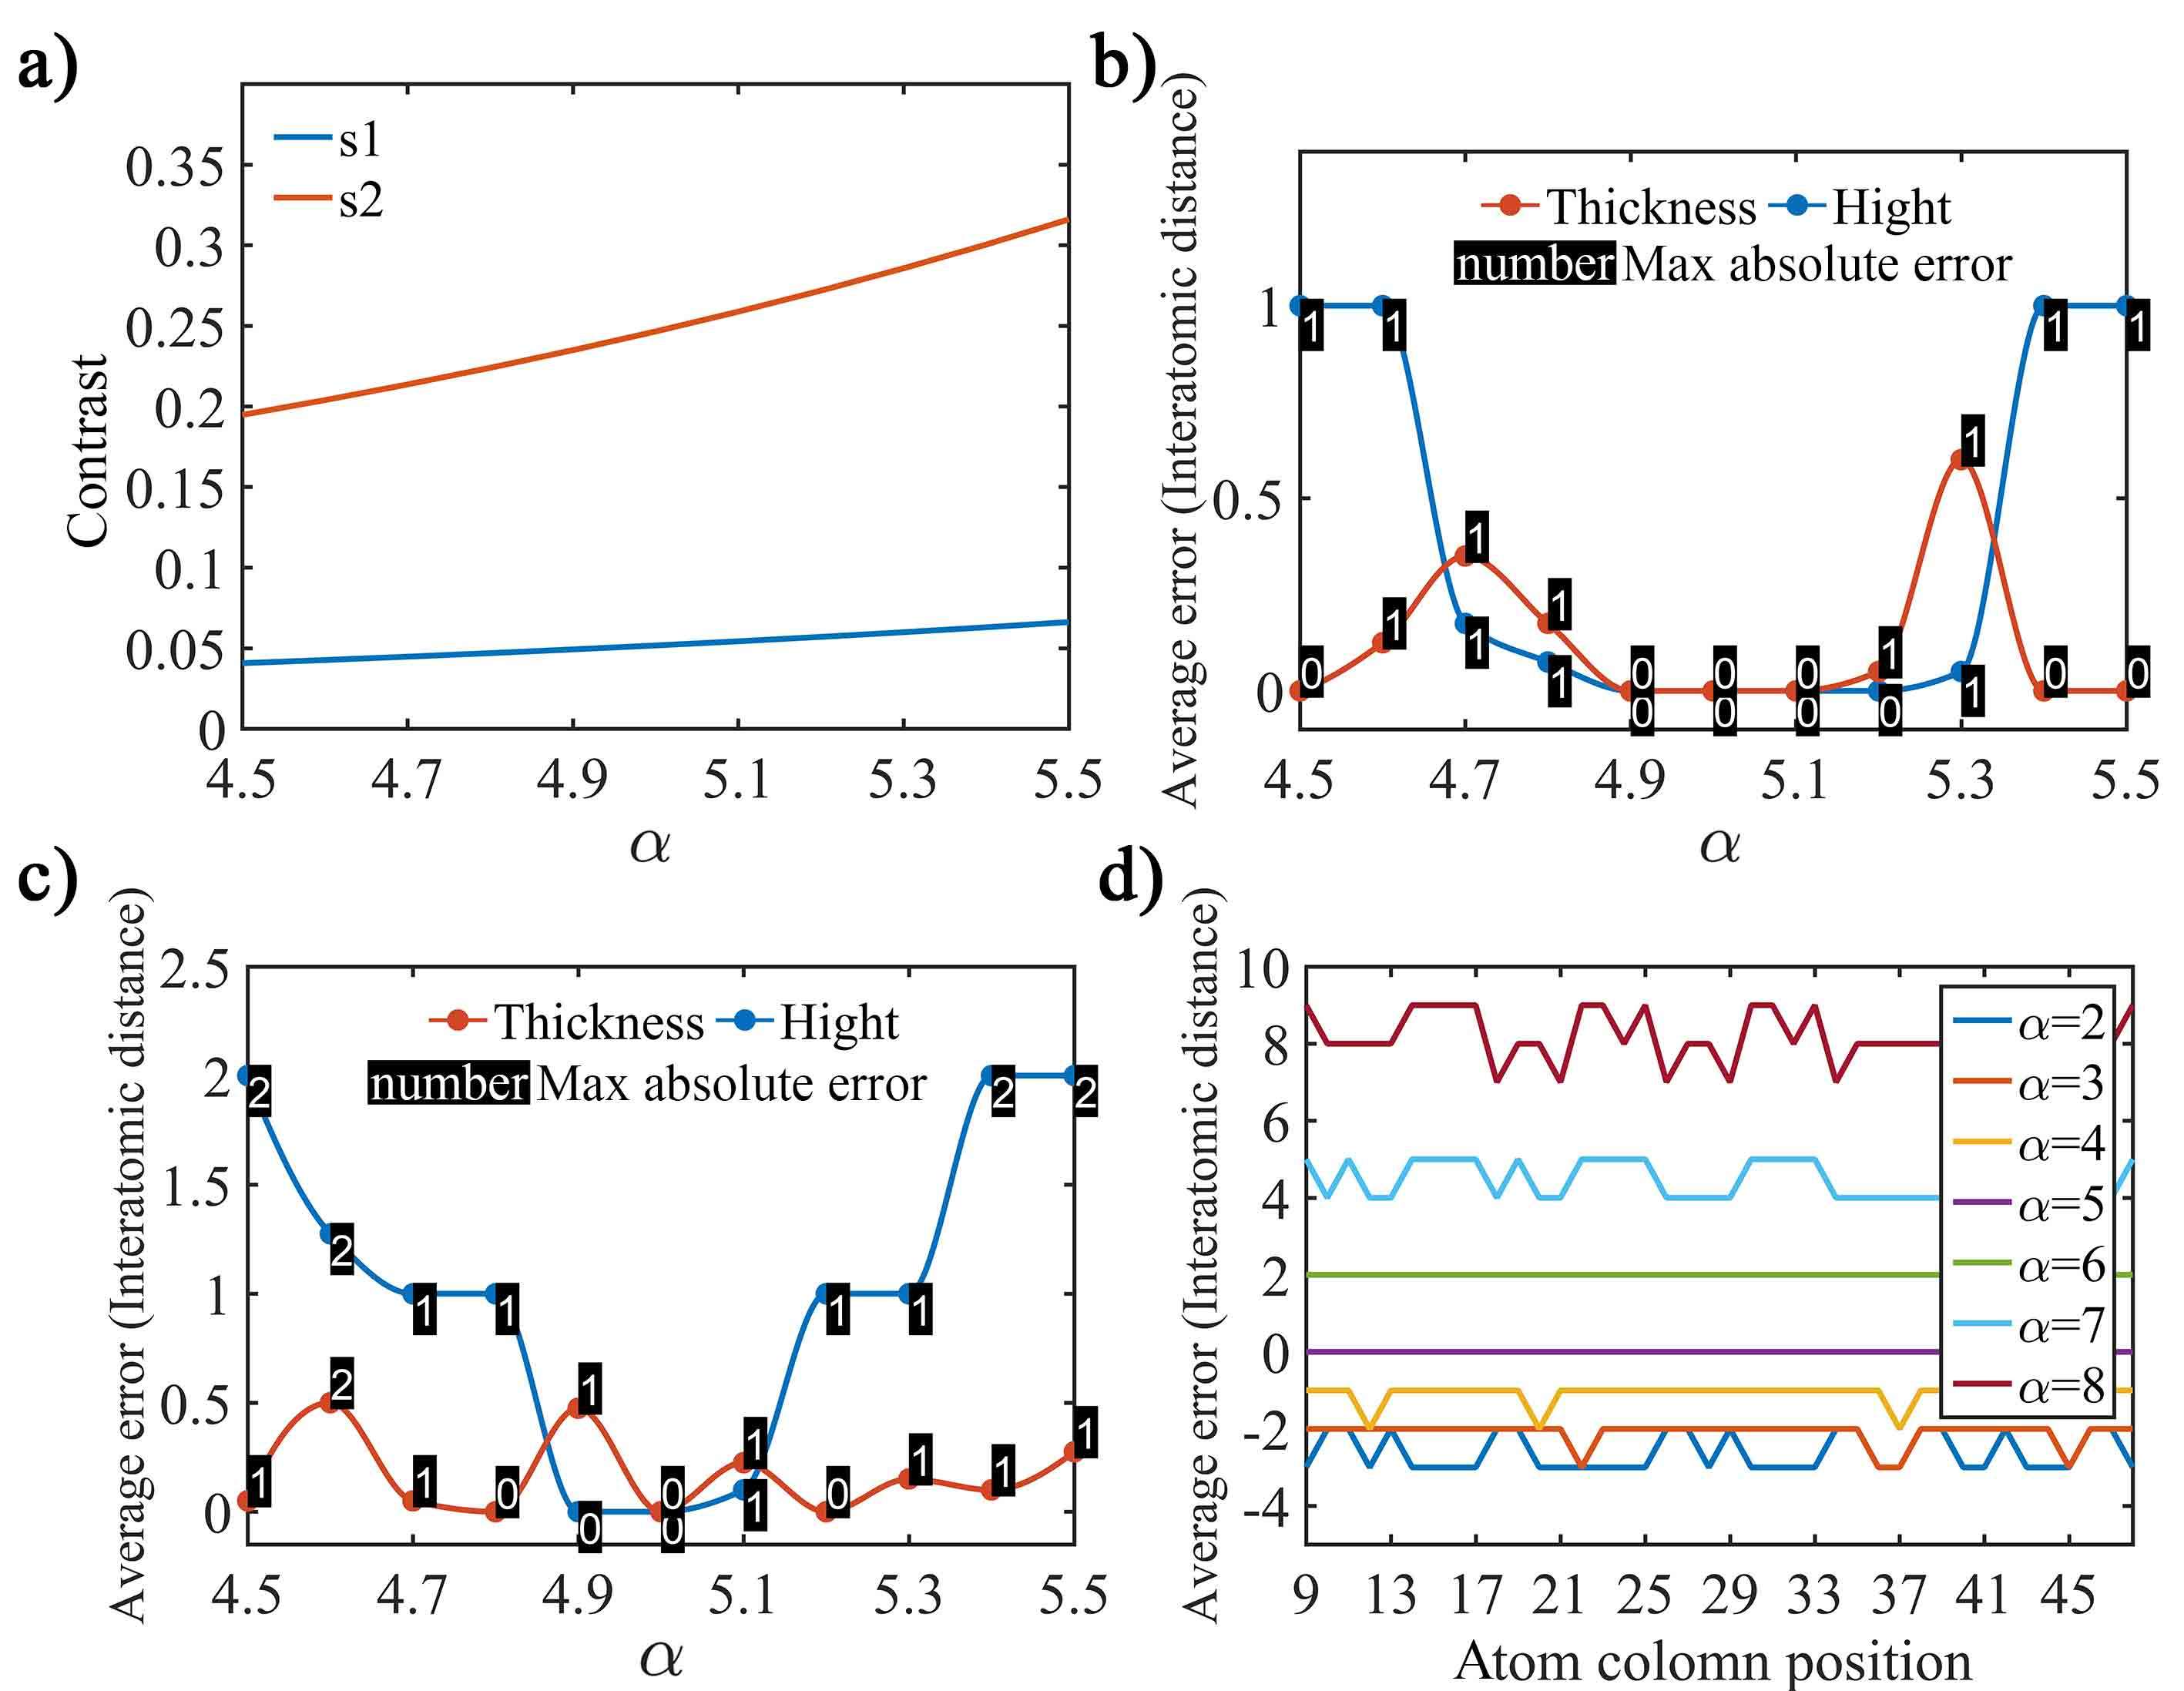
\includegraphics[width=0.8\textwidth]{../2.7/27}
 	\caption{模拟测试 MTF 对重构的影响}\label{fig:27}
 	\song\tuzhu{a) 不同 $\alpha$ 对应的 MTF 矫正 s1 和 s2 的模拟像后图像衬度的变化曲线,其中 s1 和 s2 的模拟像均加入了 $\alpha = 5$ 对应的 MTF 曲线的影响;b,c) 不同 $\alpha$ 对应的 MTF 矫正 s1 和 s2 的模拟像后的图像的重构误差曲线;d) 不同 $\alpha$ 对应的 MTF 矫正 s1 的模拟像后的图像经重构后,所有原子柱的厚度误差}
 \end{figure}
 \subsubsection{模拟测试小结}
 本节提出了从单张原子分辨 TEM 照片重构晶体材料的三维形貌的全局匹配算法。模拟测试证明了全局匹配算法比局部匹配算法的重构结果更加准确。我们还在模拟测试中分析讨论了多个因素对重构结果的影响,结果显示全局匹配算法可以适用于一般的球差矫正 TEM 拍摄得到的原子分辨率 TEM 照片。具体地,当晶体的晶带轴被校正的情况下,即使其中存在残余晶体倾转,全局匹配算法的重构精度也不会受太大影响。另外,欠焦量、三级球差、噪音等对重构精度的影响更加微弱。不过,MTF 对重构结果的影响特别明显,其在图像定量分析中是不可忽视的因素,在重构之前需要被准确地测量。

\section{三维重构方案的自洽性}
\subsection{环绕效应收敛测试}
在第 1.2.4.3 款已述及,环绕效应会导致图像模拟误差。在多层法运算过程中,每一层运算都会有误差被包裹到图像中。而这种产生于边界的误差,能够向图像内部扩散至多深,是相当复杂的一个问题,取决于样品厚度、成像条件等诸多因素。因此,为了保证全局匹配算法中图像模拟的精确性,必须避免这种由图像计算时的周期性假设所导致的误差。这意味着,在模拟感兴趣区域的高分辨 TEM 照片时使用的超胞模型必须大于感兴趣区域,以阻挡环绕效应影响到感兴趣区域的图像衬度。而在图像匹配时,只使用感兴趣区域的图像与实验图像对比。如图 4.9 所示,为了确定超胞模型的必要尺寸,我们对不同大小的模型进行了收敛测试。

在收敛测试中,如图 4.9a 所示,我们将感兴趣区域的超胞标记为 \textbf{0},将一系列不同尺寸的超胞标记为 \textbf{0},\textbf{1},…,\textbf{6}。接着,计算出这些超胞的模拟像 $I_i(x, y)(i = 0,\cdots, n)$,这些图像的尺寸当然也各不相同。对于连续的两张图像,我们在图像 $I_0$ 对应的区域计算出它们的差 $\Delta I_i(x, y) = I_{i+1}(x, y)$ – $I_i(x, y)$,如图 4.9b 所示。图 4.9c 是图 4.9b 中每个图像的标准差。根据图 4.9b 和 c 可以得出以下结论:(1)当超胞的尺寸由 \textbf{0} 增大到 \textbf{1} 时,图像的强度在边界处发生了强烈的变化,这意味着超胞 \textbf{0} 所产生的环绕效应主要集中在其边界;(2)超胞 \textbf{1} 或 \textbf{2} 已经足够大,继续增加超胞的尺寸不会对误差产生显著的改善作用,标准差也已经在此时接近收敛。

\begin{figure}[htbp]
	\vspace{\baselineskip}
	\centering
	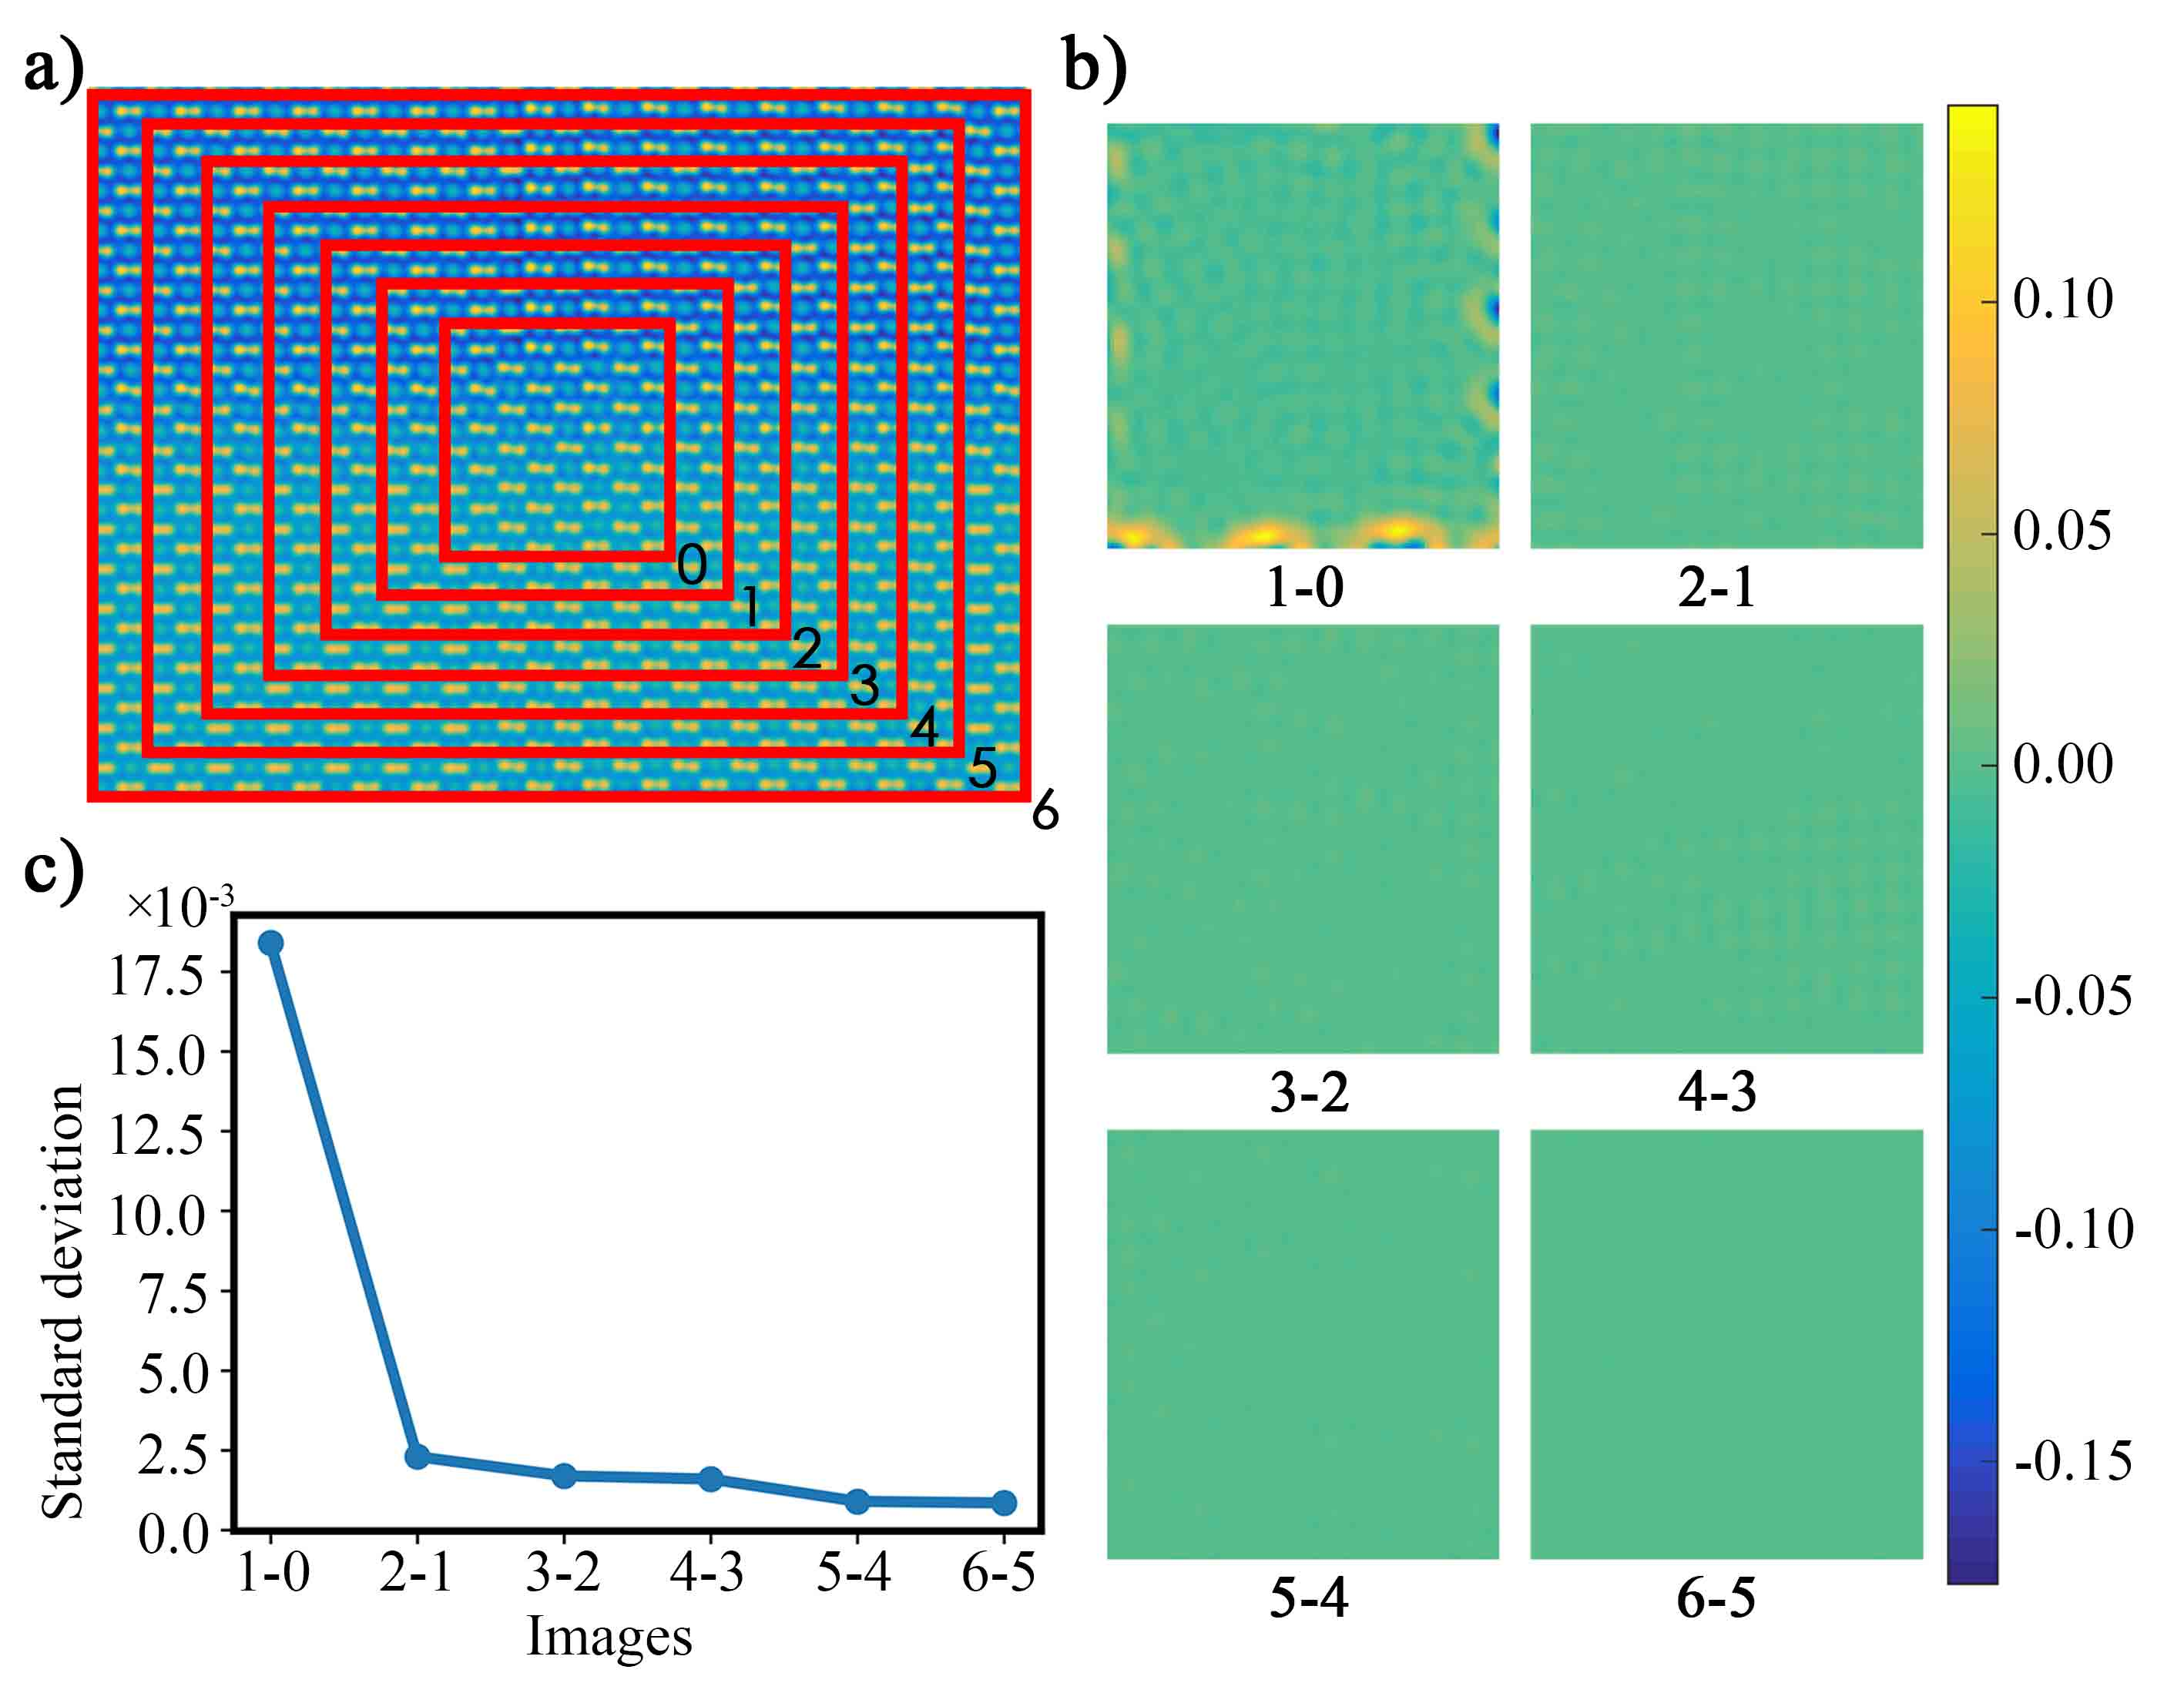
\includegraphics[width=0.8\textwidth]{../2.8/28}
	\caption{环绕效应收敛测试示意图}\label{fig:28}
	\song\tuzhu{a) 表面倾斜的 Si 超胞的模拟像,其中红色矩形框标记了不同尺寸的超胞,超胞 \textbf{0} 至超胞 \textbf{6} 尺寸依次增大;b) 两个连续超胞的模拟像的差,图像仅在超胞 \textbf{0} 所在的区域进行对比;c) 图 b 中每张图像的标准差的变化曲线}
\end{figure}

\subsection{自洽性验证及分辨率}
我们引入了一个自洽性验证方案以保证全局匹配算法结果的有效性,并且定义了三维重构在 $z$ 方向上的分辨率。通过自洽性验证方案得到的结果将更为客观,操作者对结果的影响程度将大幅降低。该方案的主要思想如图 4.10 所示,在实际三维重构时,即使所需重构的感兴趣区域已经确定,仍然存在许多种超胞的选取方式,即可选区不同的实验图像区域。比如,图 4.10 中红色矩形框所围的区域 A1(右上角标记)是一种超胞的选取方式。其他还存在一些相同尺寸的超胞选取方式,比如 A2,A3,B1,B2 等。问题的关键是,不同的超胞可能会导致最终重构的感兴趣区域的原子结构略有不同。这是因为同一个感兴趣区域在不同的超胞中具有略微不同的环境,这有可能导致不同的重构误差。举例来说,用全局匹配算法重构感兴趣区域(图 4.10 中橙色区域)时,由超胞 A1 重构所得的结果和由超胞 C5 重构所得的结果,有可能会略有差别。因为除了图 4.10 中的黄色区域是 A1 和 C5 共有的区域外,它们在其他区域具有不同的局部样品厚度、欠焦量以及非晶覆盖状况等。这种环境的差异会造成最终重构结果的差异。所以,原则上某一感兴趣区域的重构应该综合多个独立的重构结果,最终的重构结果应该是这些不同的重构结果的平均。如此所得的平均结果更加客观,消除人为操作对结果的影响,而且可以验证重构结果的合理性。
比较感兴趣区域中每一个原子柱的平均厚度和平均高度和每个独立重构结果的差别可以获得厚度和高度的重构误差。通过统计所有独立重构的结果中所有原子柱处的误差,我们可以以如下的方式定义三维重构在 $z$ 方向上的分辨率:首先去除所有误差中前 20\% 的较大误差,然后将剩余的 80\% 的误差中的最大值定义为三维重构在 $z$ 方向上的分辨率。比如,如果在对某一感兴趣区域的重构中产生的所有误差中,有少于 20\% 的误差大于或等于 2 个原子间距,而超过 80\% 的误差都小于 2 个原子间距,则定义该三维重构在 $z$ 方向上的分辨率是 1 个原子间距。
\begin{figure}[htbp]
	\vspace{\baselineskip}
	\centering
	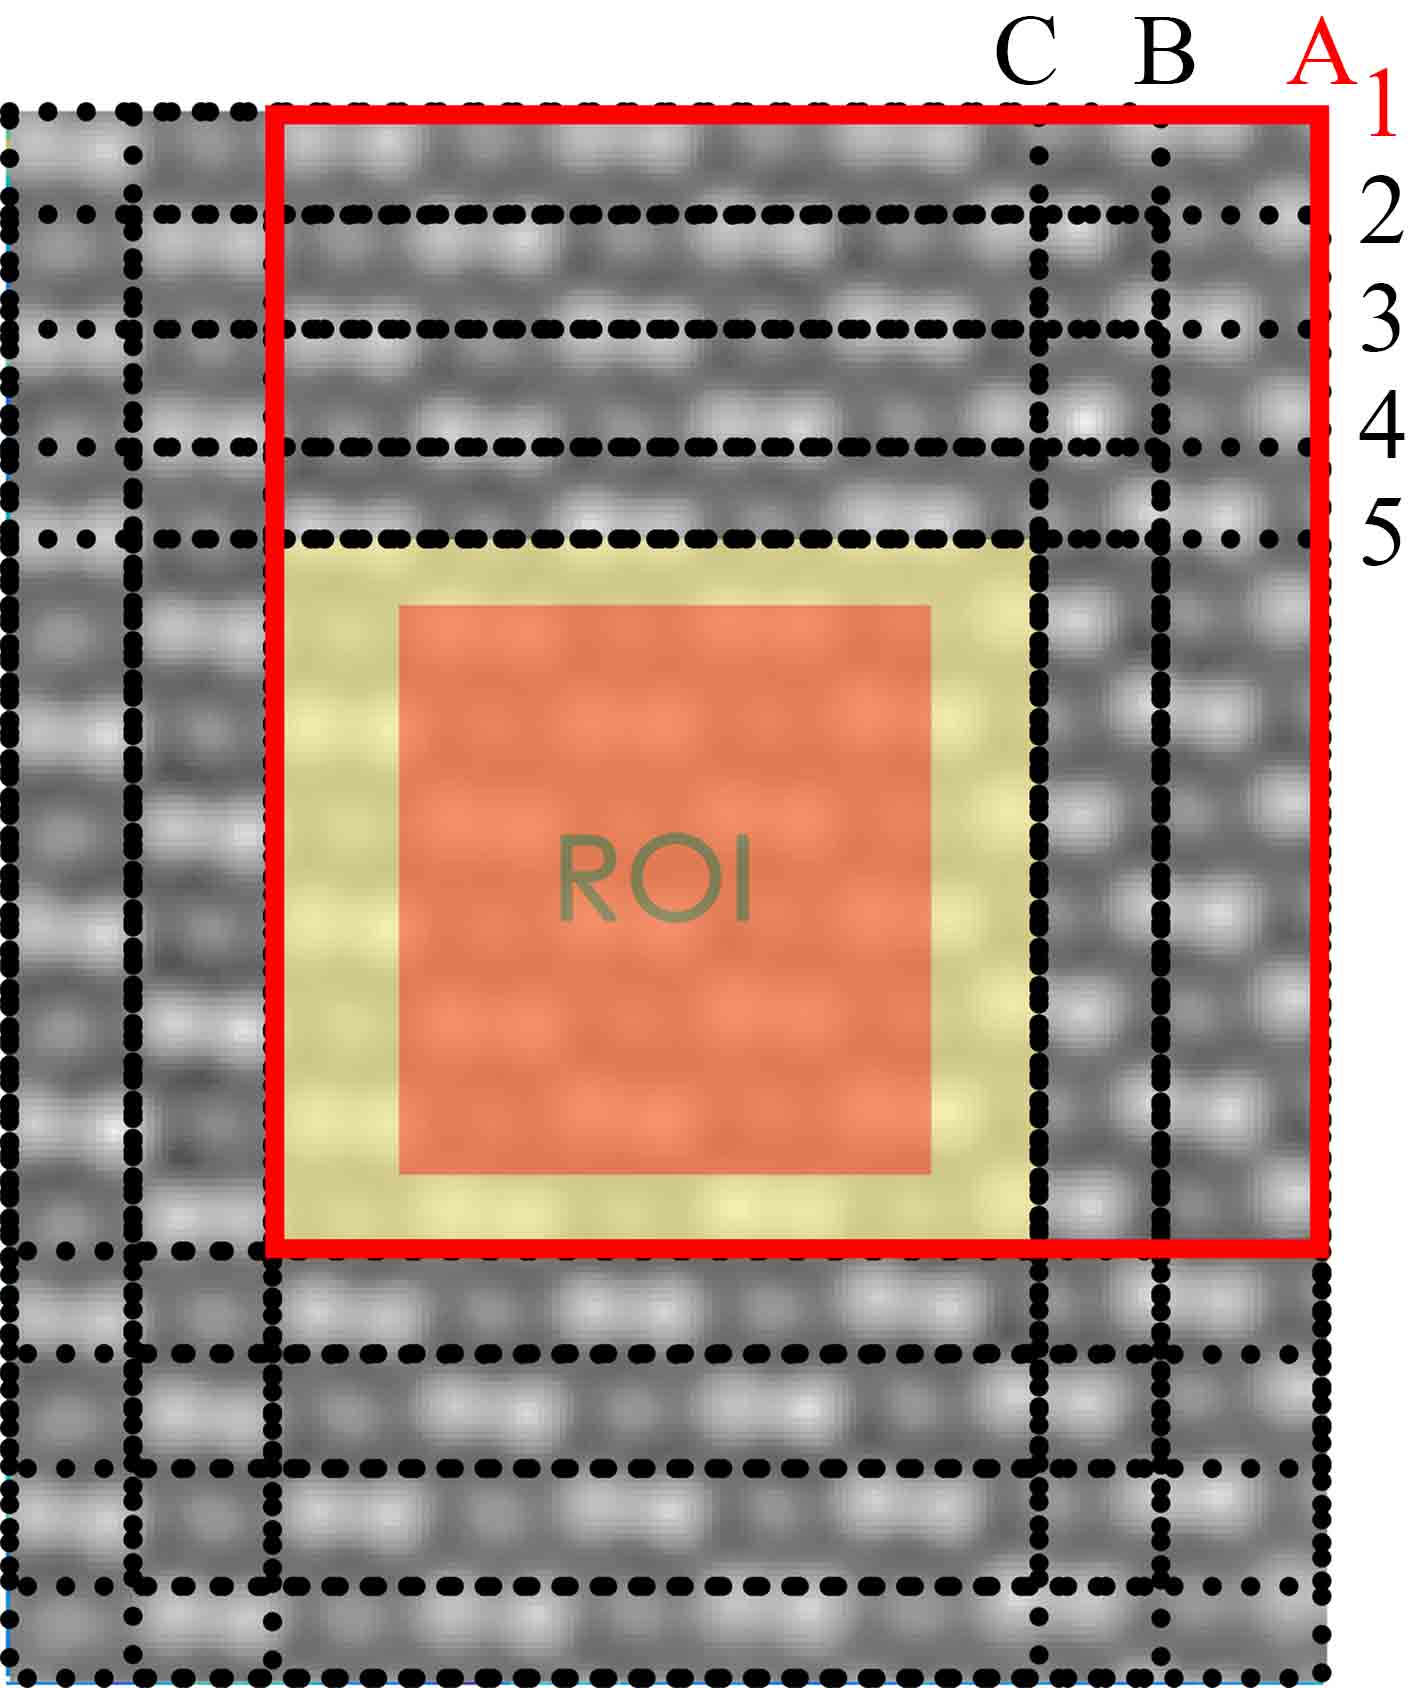
\includegraphics[width=0.4\textwidth]{../2.9/29}
	\caption{自洽性验证方案分区图}\label{fig:29}
	\song\tuzhu{图中展示了相同尺寸但是位置不同的超胞 A1, A2 … C5 的选区方式,这些超胞均具有相同的公共区域,右上角是不同超胞的命名方式}
\end{figure}

\subsection{非晶对重构的影响}
由于非晶对样品的污染在大部分的实验中是不可避免的,但是又无法将其考虑到重构的过程中,因此有必要定量估算其对图像衬度的影响。为了模拟非晶对一般晶体材料高分辨电镜照片图像强度的影响,我们构建了一个尺寸为 $9.7 \textnormal{ nm} \times 9.7 \textnormal{ nm} \times 4.3 \textnormal{ nm}$ 的 Si  超胞。如图 4.11d 所示,该超胞的 $z$ 方向沿晶体的 [100] 方向,在晶体上下表面分别为其覆盖上厚度为 0.0,0.5,1.0,1.5,2.0 以及 2.5 nm 的非晶层。其中 Si 非晶层中的原子位置是通过分子动力学模拟软件 LAMMPS,根据 T. Grieb 等工作~\cite{Grieb2018}中的方式计算所得。图 4.11a-c 直观地展示了当表面非晶层增厚时,所得的高分辨电镜照片的图像衬度变化之明显。图 4.11e 进一步展示了由非晶层导致的图像强度误差相对于非晶层厚度的变化曲线。从以上的对比可知,非晶对图像强度的影响是非常显著的,所以这些影响必须被仔细地分析以保证重构算法可以被正确地应用于实际材料的重构。值得注意的是,由于被非晶影响的高分辨电镜照片的噪音比较严重,在将这些照片与单纯晶体的高分辨电镜照片对比之前,这些照片都通过了 Weiner 滤波器~\cite{Kilaas1998}的过滤(电镜照片定量分析中经常执行的一个步骤),以减轻噪音的影响。实际上,Weiner 滤波器是一种在倒空间中去除图像背底噪音和提高图像质量的方法,它并不能完全消除非晶对图像衬度的影响,比如图 4.11b 和 c 与图 4.11a 依然具有很大的差别。

\begin{figure}[htbp]
	\vspace{\baselineskip}
	\centering
	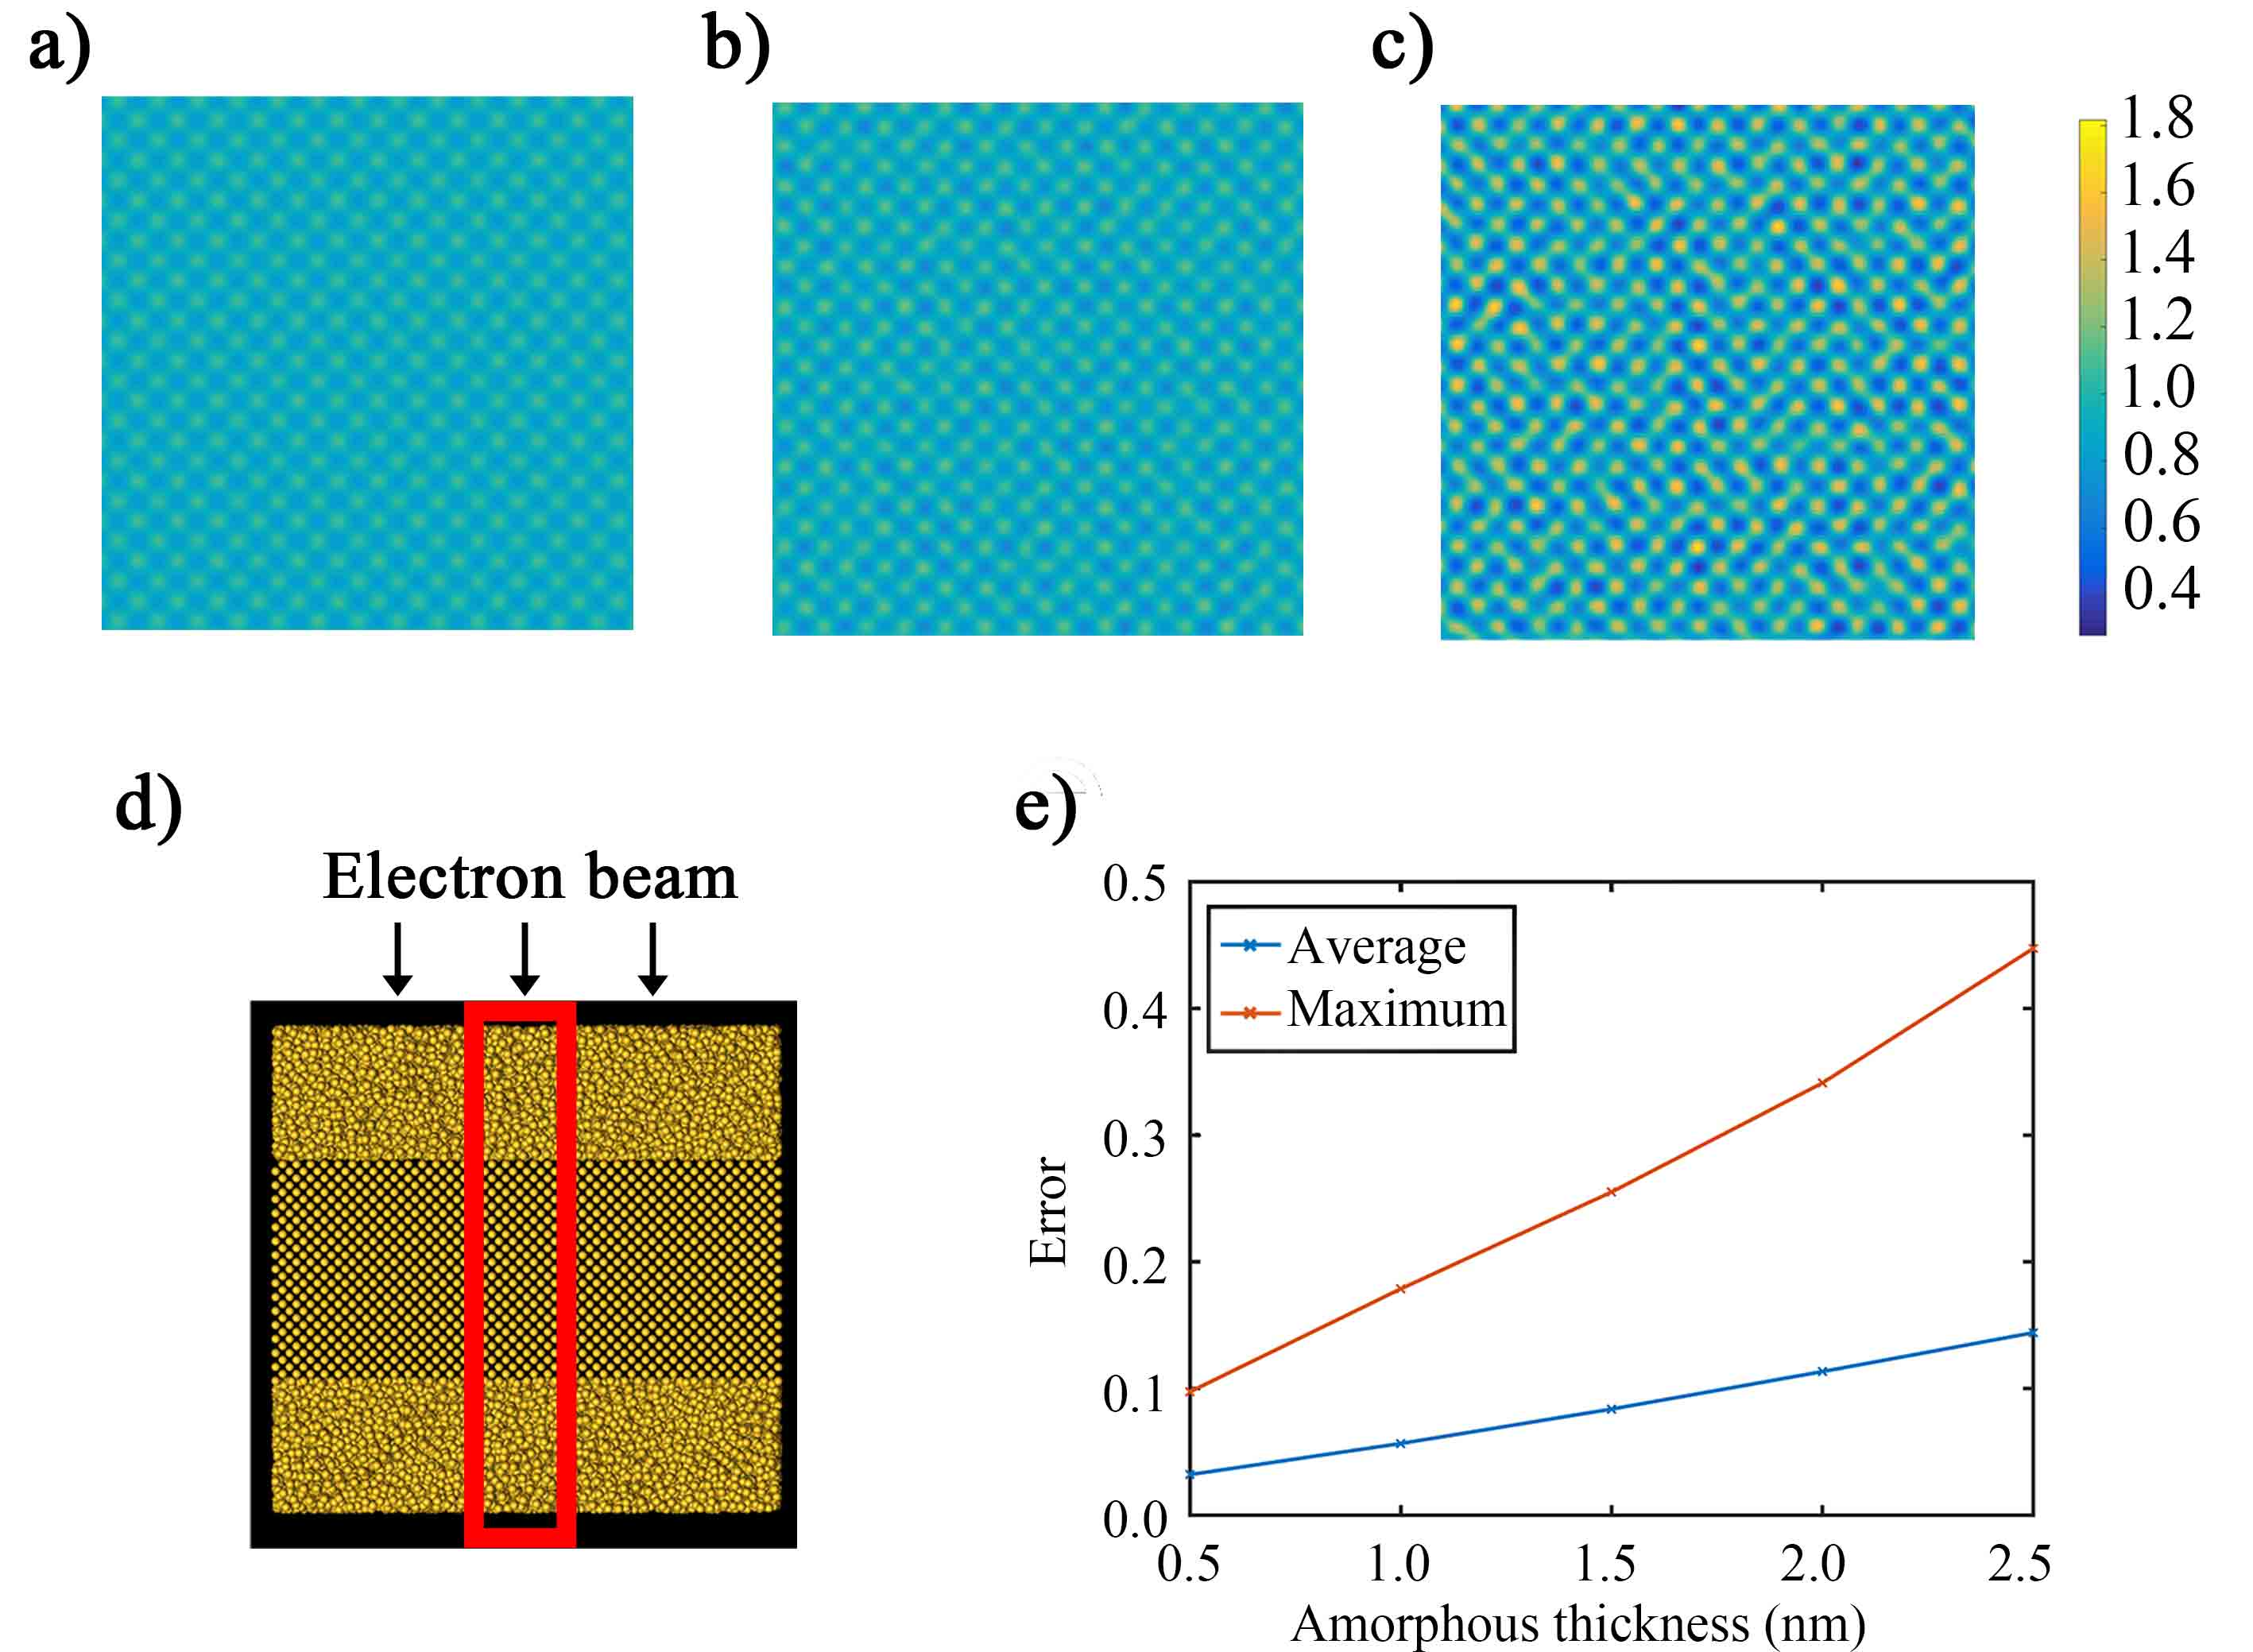
\includegraphics[width=0.7\textwidth]{../2.10/210}
	\caption{非晶对图像衬度的影响}\label{fig:210}
	\song\tuzhu{a-c) Si[100] 的高分辨电镜照片模拟像,其中 Si 晶体的上下表面覆盖了厚度为 0.0,0.5,2.5 nm 的非晶层,这些图片均通过 Weiner 滤波器过滤;d) Si[100] 样品的截面图,Si 晶体上下覆盖了等厚的非晶层,其中 Si 晶体的尺寸为 $9.7 \textnormal{ nm} \times 9.7 \textnormal{ nm} \times 4.3 \textnormal{ nm}$,电子束沿 Si[100] 入射,只有红色矩形框中的区域的模拟像展示于图 a-c 中;e) 覆盖非晶后的超胞的模拟像与 Si 晶体模拟像之间的平均误差与最大误差相对于非晶厚度的变化曲线}
\end{figure}

如图 4.11e 所示,当非晶层增厚时,最大误差增长的幅度比平均误差增长的幅度更大,所以其中大误差的具体分布情况需要进一步的分析。图 4.12a 和 b 展示了当非晶厚度为 0.5 nm 时,大误差(红色标记所示,绝对值超过 0.1)相对于 Si[100] 投影势场的分布情况。从中可以发现,当非晶层较薄时,其引入的大误差大部分分布于原子柱之间,只有小部分的大误差分布于接近原子柱的位置。从图 4.12c 和 d 中的误差分布直方图可知,当非晶层很薄时(比如 0.5 nm),其产生的误差几乎不超过 0.1。但是当非晶层厚度增加至 2.5 nm 时,其引入的误差大部分都会超过 0.1,此时的误差将随机分布于整个区域。

\begin{figure}[htbp]
	\vspace{\baselineskip}
	\centering
	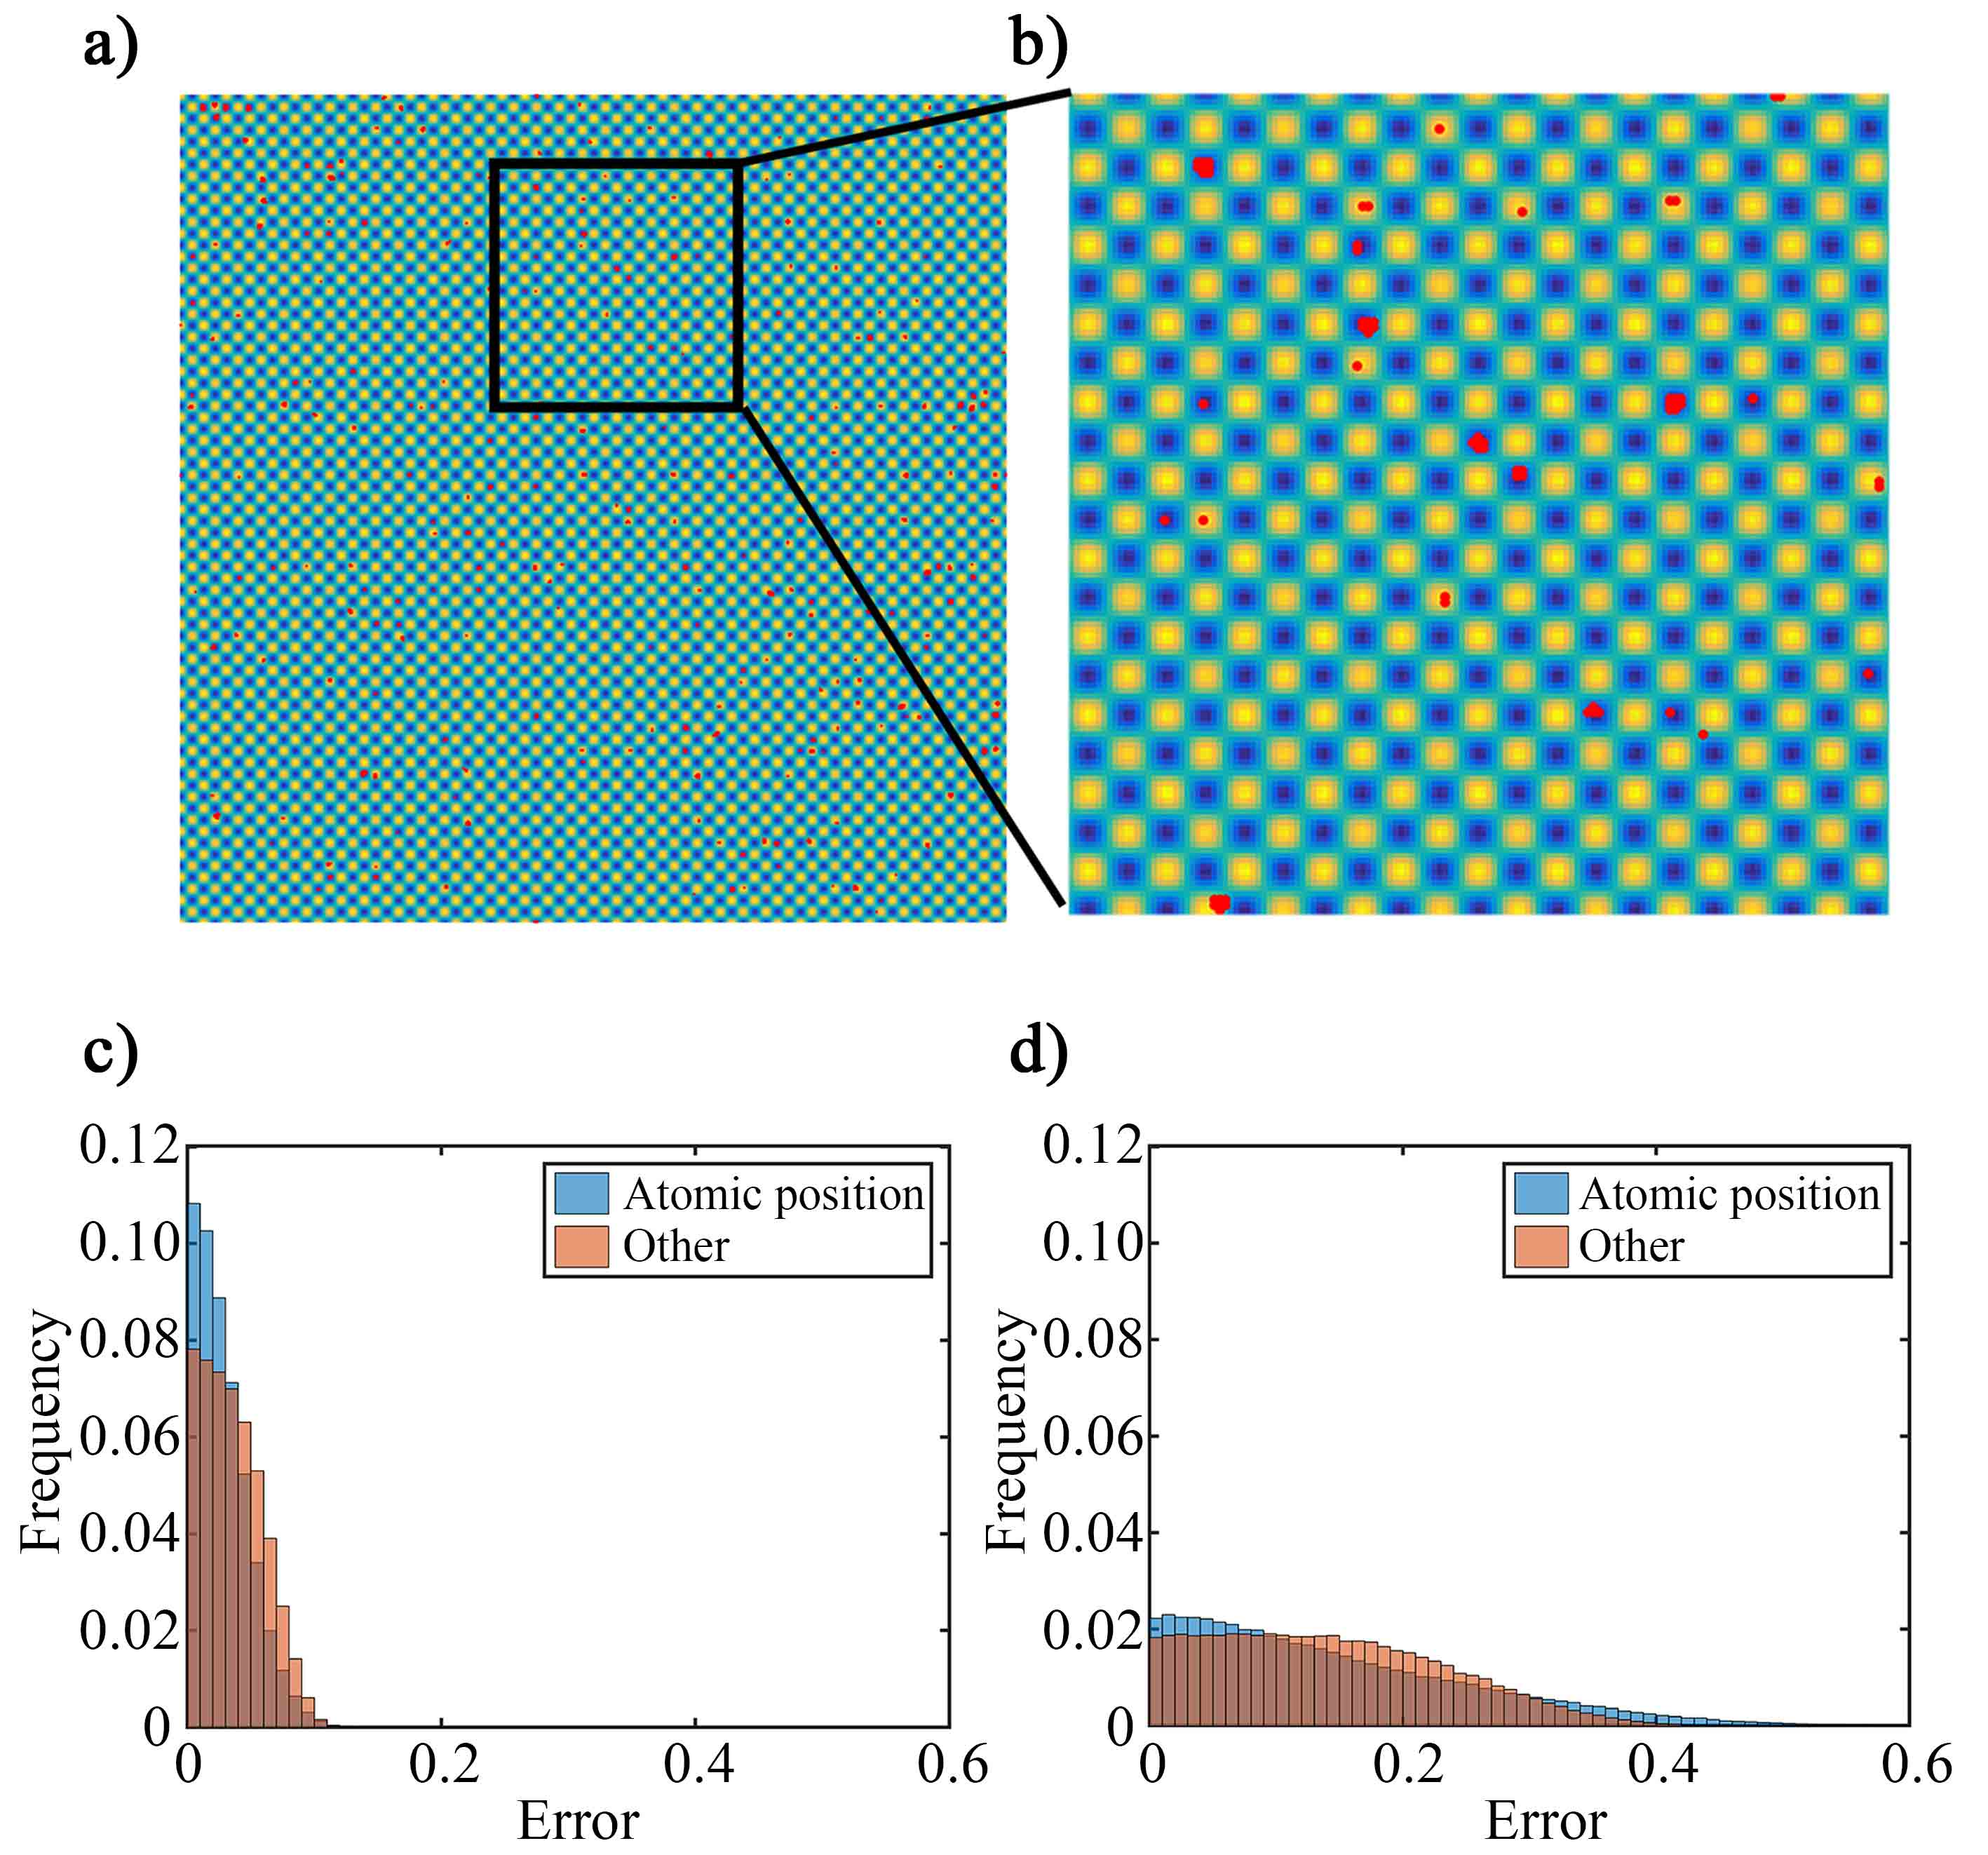
\includegraphics[width=0.9\textwidth]{../2.11/211}
	\caption{非晶引起的误差分布示意图}\label{fig:211}
	\song\tuzhu{a) 图 4.11a 与图 4.11b 之间较大误差的分布情况示意图,其中误差绝对值大于 0.1 的区域被标记为红色;b) 图 a 中线框区域的放大图;c,d) 图 4.11a 与图 4.11b 以及图 4.11a 与图 4.11c 之间的误差的分布直方图}
\end{figure}

\subsection{三维重构的置信度}
为了测量全局匹配算法重构的可靠性以及其对一般材料和一般原子分辨率图像的适用性,在此定义置信度 $C_{3D}$ 如下:
\begin{equation}
C_{3D}=1-E_{average}-E_{column}
\end{equation}
其中 $E_{average}$ 是整张图像的平均误差与整张实验图像的平均图像强度的比值,$E_{column}$ 是原子柱位置的平均误差与原子柱位置的平均图像强度的比值。实际上,第一项 $E_{average}$ 已经包含了第二项 $E_{column}$ 中的误差,但是原子柱位置的误差相比于原子柱位置之间的误差对重构结果的影响更大,所以将该类误差在置信度中的权重加倍。可以合理推断,误差越小,重构的置信度就应该越高。当误差全部由非晶引起时, $C_{3D}$ 直接与非晶层的厚度呈负相关,如图 4.13a 所示。随着非晶层由 0 增加至 $1.5 \textnormal{ nm}$,三维重构的置信度将从 100\% 快速下降到 90\% 以下。一个好的三维重构结果,它的置信度应该保持在 90\% 以上。



需要指出的是,尽管非晶污染是实际实验中最难以控制的误差来源,其他的因素,例如成像条件偏离最佳等等也是产生误差的原因。任何使图像质量变差的因素都将降低三维重构结果的置信度。再次强调,在估计置信度时,原子柱位置的误差应该被加倍考虑,因为此处的误差对重构可靠性的影响最严重。

\begin{figure}[htbp]
	\vspace{\baselineskip}
	\centering
	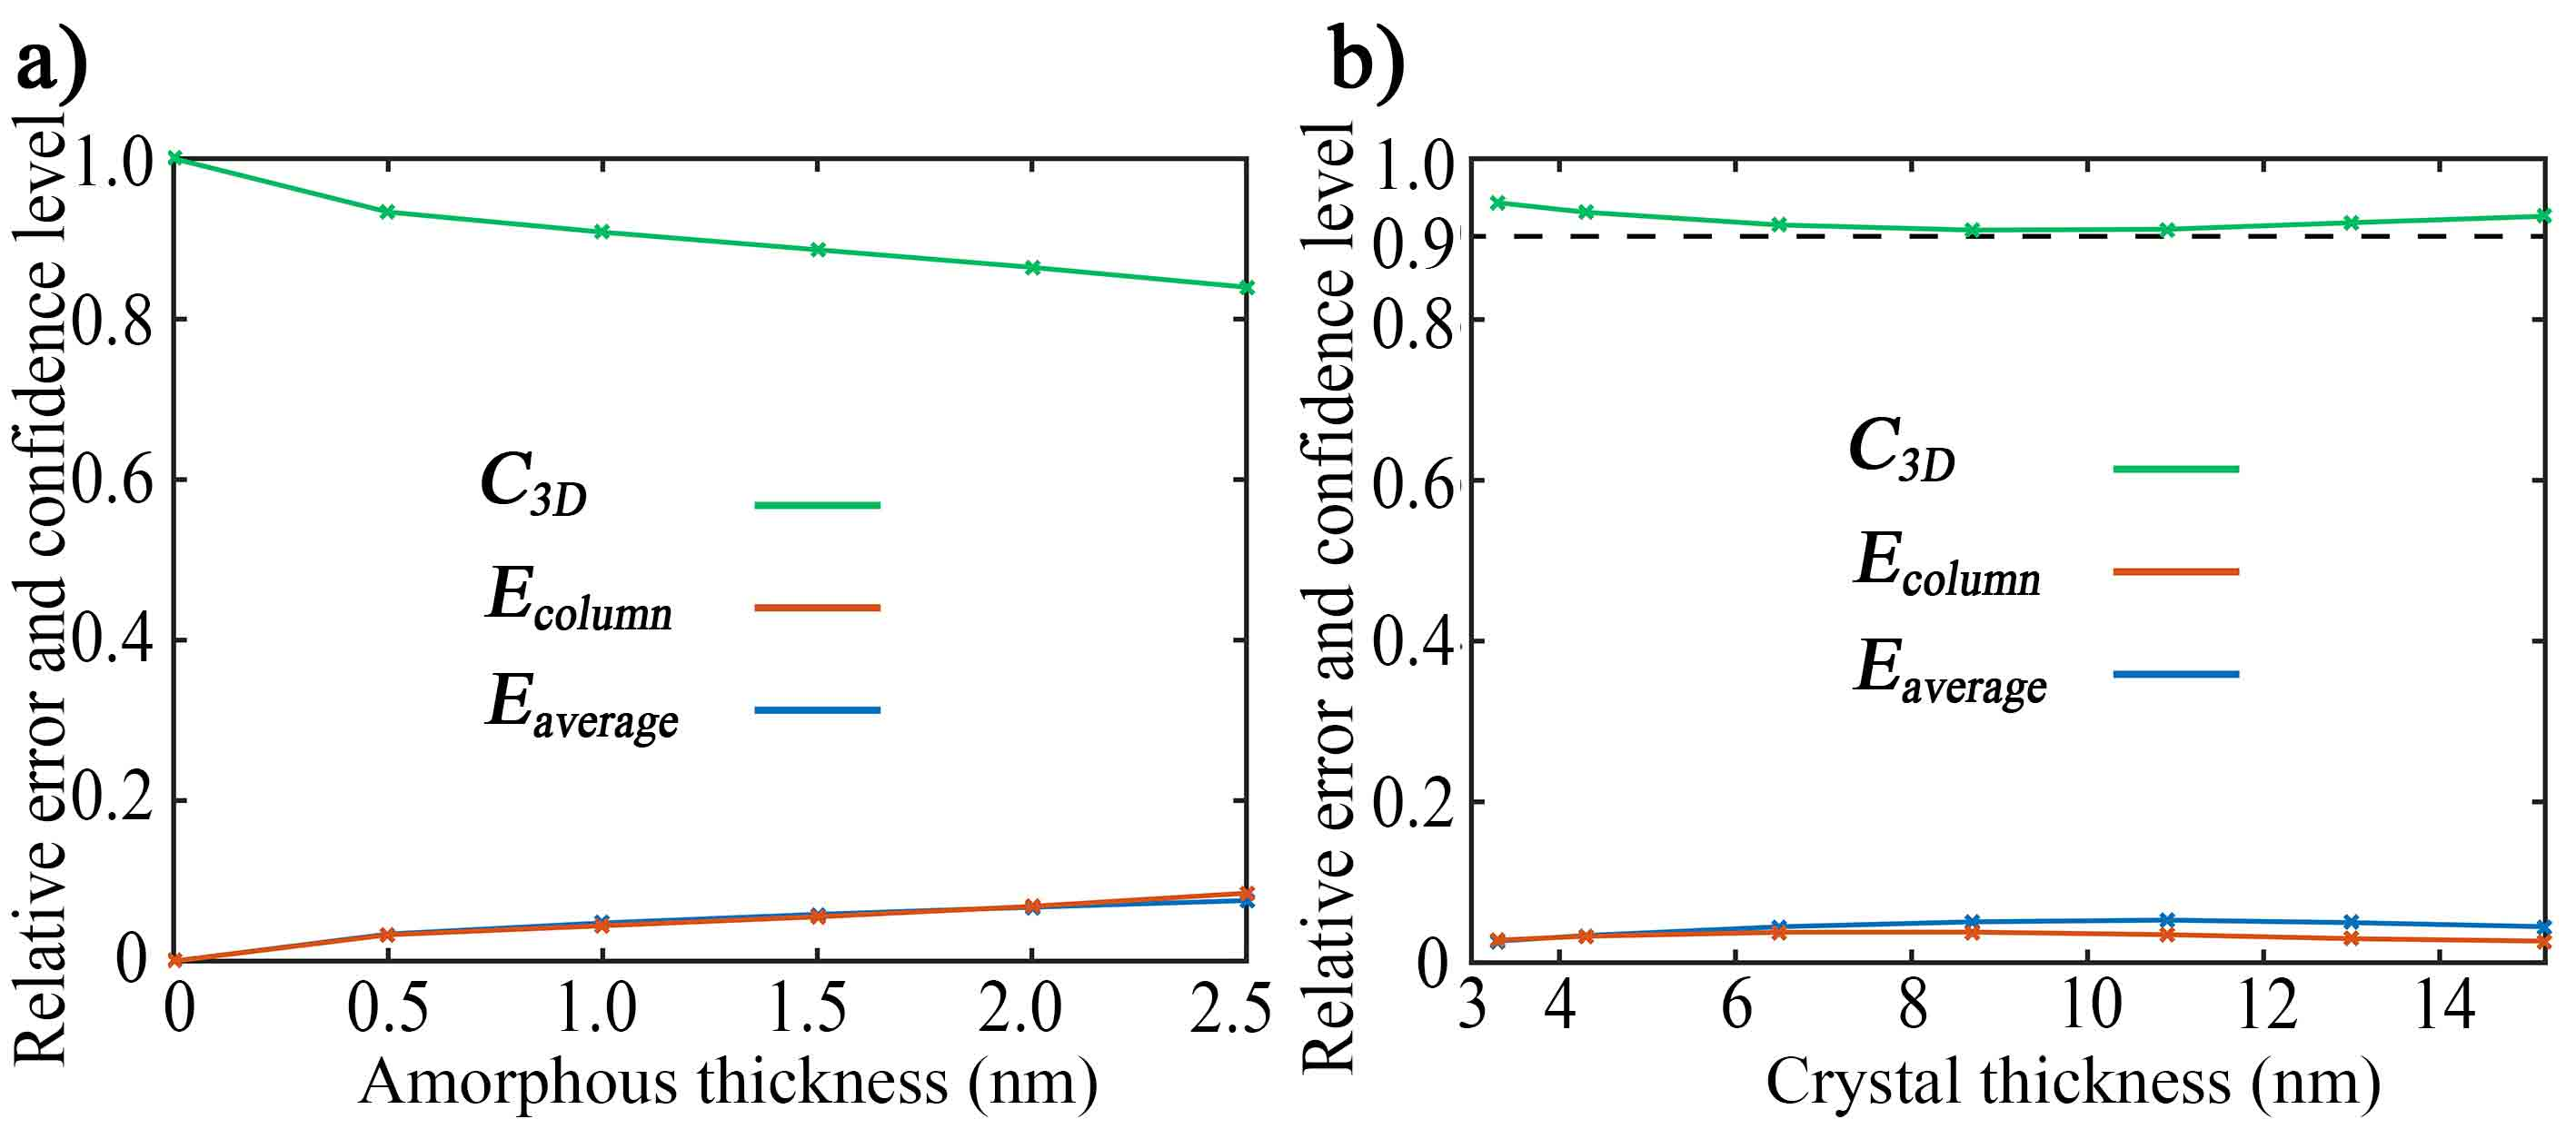
\includegraphics[width=0.9\textwidth]{../2.12/212}
	\caption{置信度关于非晶以及晶体厚度的变化关系}\label{fig:212}
	\song\tuzhu{a) 当晶体厚度为 4 nm 时,置信度关于非晶层厚度的变化曲线;b) 当非晶层厚度为 0.5 nm 时,置信度关于晶体厚度的变化曲线;所有的模拟都在球差和欠焦量都为 0 的条件下进行计算,所有误差均全部有非晶引起}
\end{figure}

\section{实验图像的三维重构}
在这一节中,我们将自洽性验证的三维重构方案应用于一张 Si[110] 的二维原子分辨率 TEM 照片,重构出了该样品的表面三维原子形貌,且重构获得了很高的分辨率和置信度。
\subsection{实验方案}
根据 C.H. Liu 等的研究~\cite{Liu2011},在 Al-Si 合金的热处理过程中,粗大的共晶 Si 颗粒的边缘会析出细小的纳米 Si 颗粒。这种纳米 Si 颗粒的尺寸非常小,适合 TEM 的观察,在球差矫正的高分辨 TEM 下可以拍摄得到高质量的原子分辨率照片。Al-Si 合金的 TEM 样品通过机械抛光和电解双喷制备,纳米 Si 颗粒出现在 Al 基体穿孔的边缘。用于观察 Si 样品的 TEM 型号是 Thermo Fisher FEI Titan 80-300 球差矫正 TEM。电镜照片沿 Si[110] 方向拍摄,详细的实验成像参数如表 4.3 所示。为了获得高质量的原子分辨率 TEM 照片,实验时使用了 NCSI 技术。$\textnormal{图 4.14a 和 b}$ 展示了拍摄到的实验照片,其中的亮点表示 Si 原子柱。在此图中,所有的 Si 原子柱在 $x-y$ 平面的位置都可以通过高斯拟合等方法确定~\cite{Garbrecht2011,Zhang2019}。相比于模拟像,该实验图像的噪音非常严重,这主要因为样品的表面存在一定的非晶污染。

\begin{figure}[htbp]
	\vspace{\baselineskip}
	\centering
	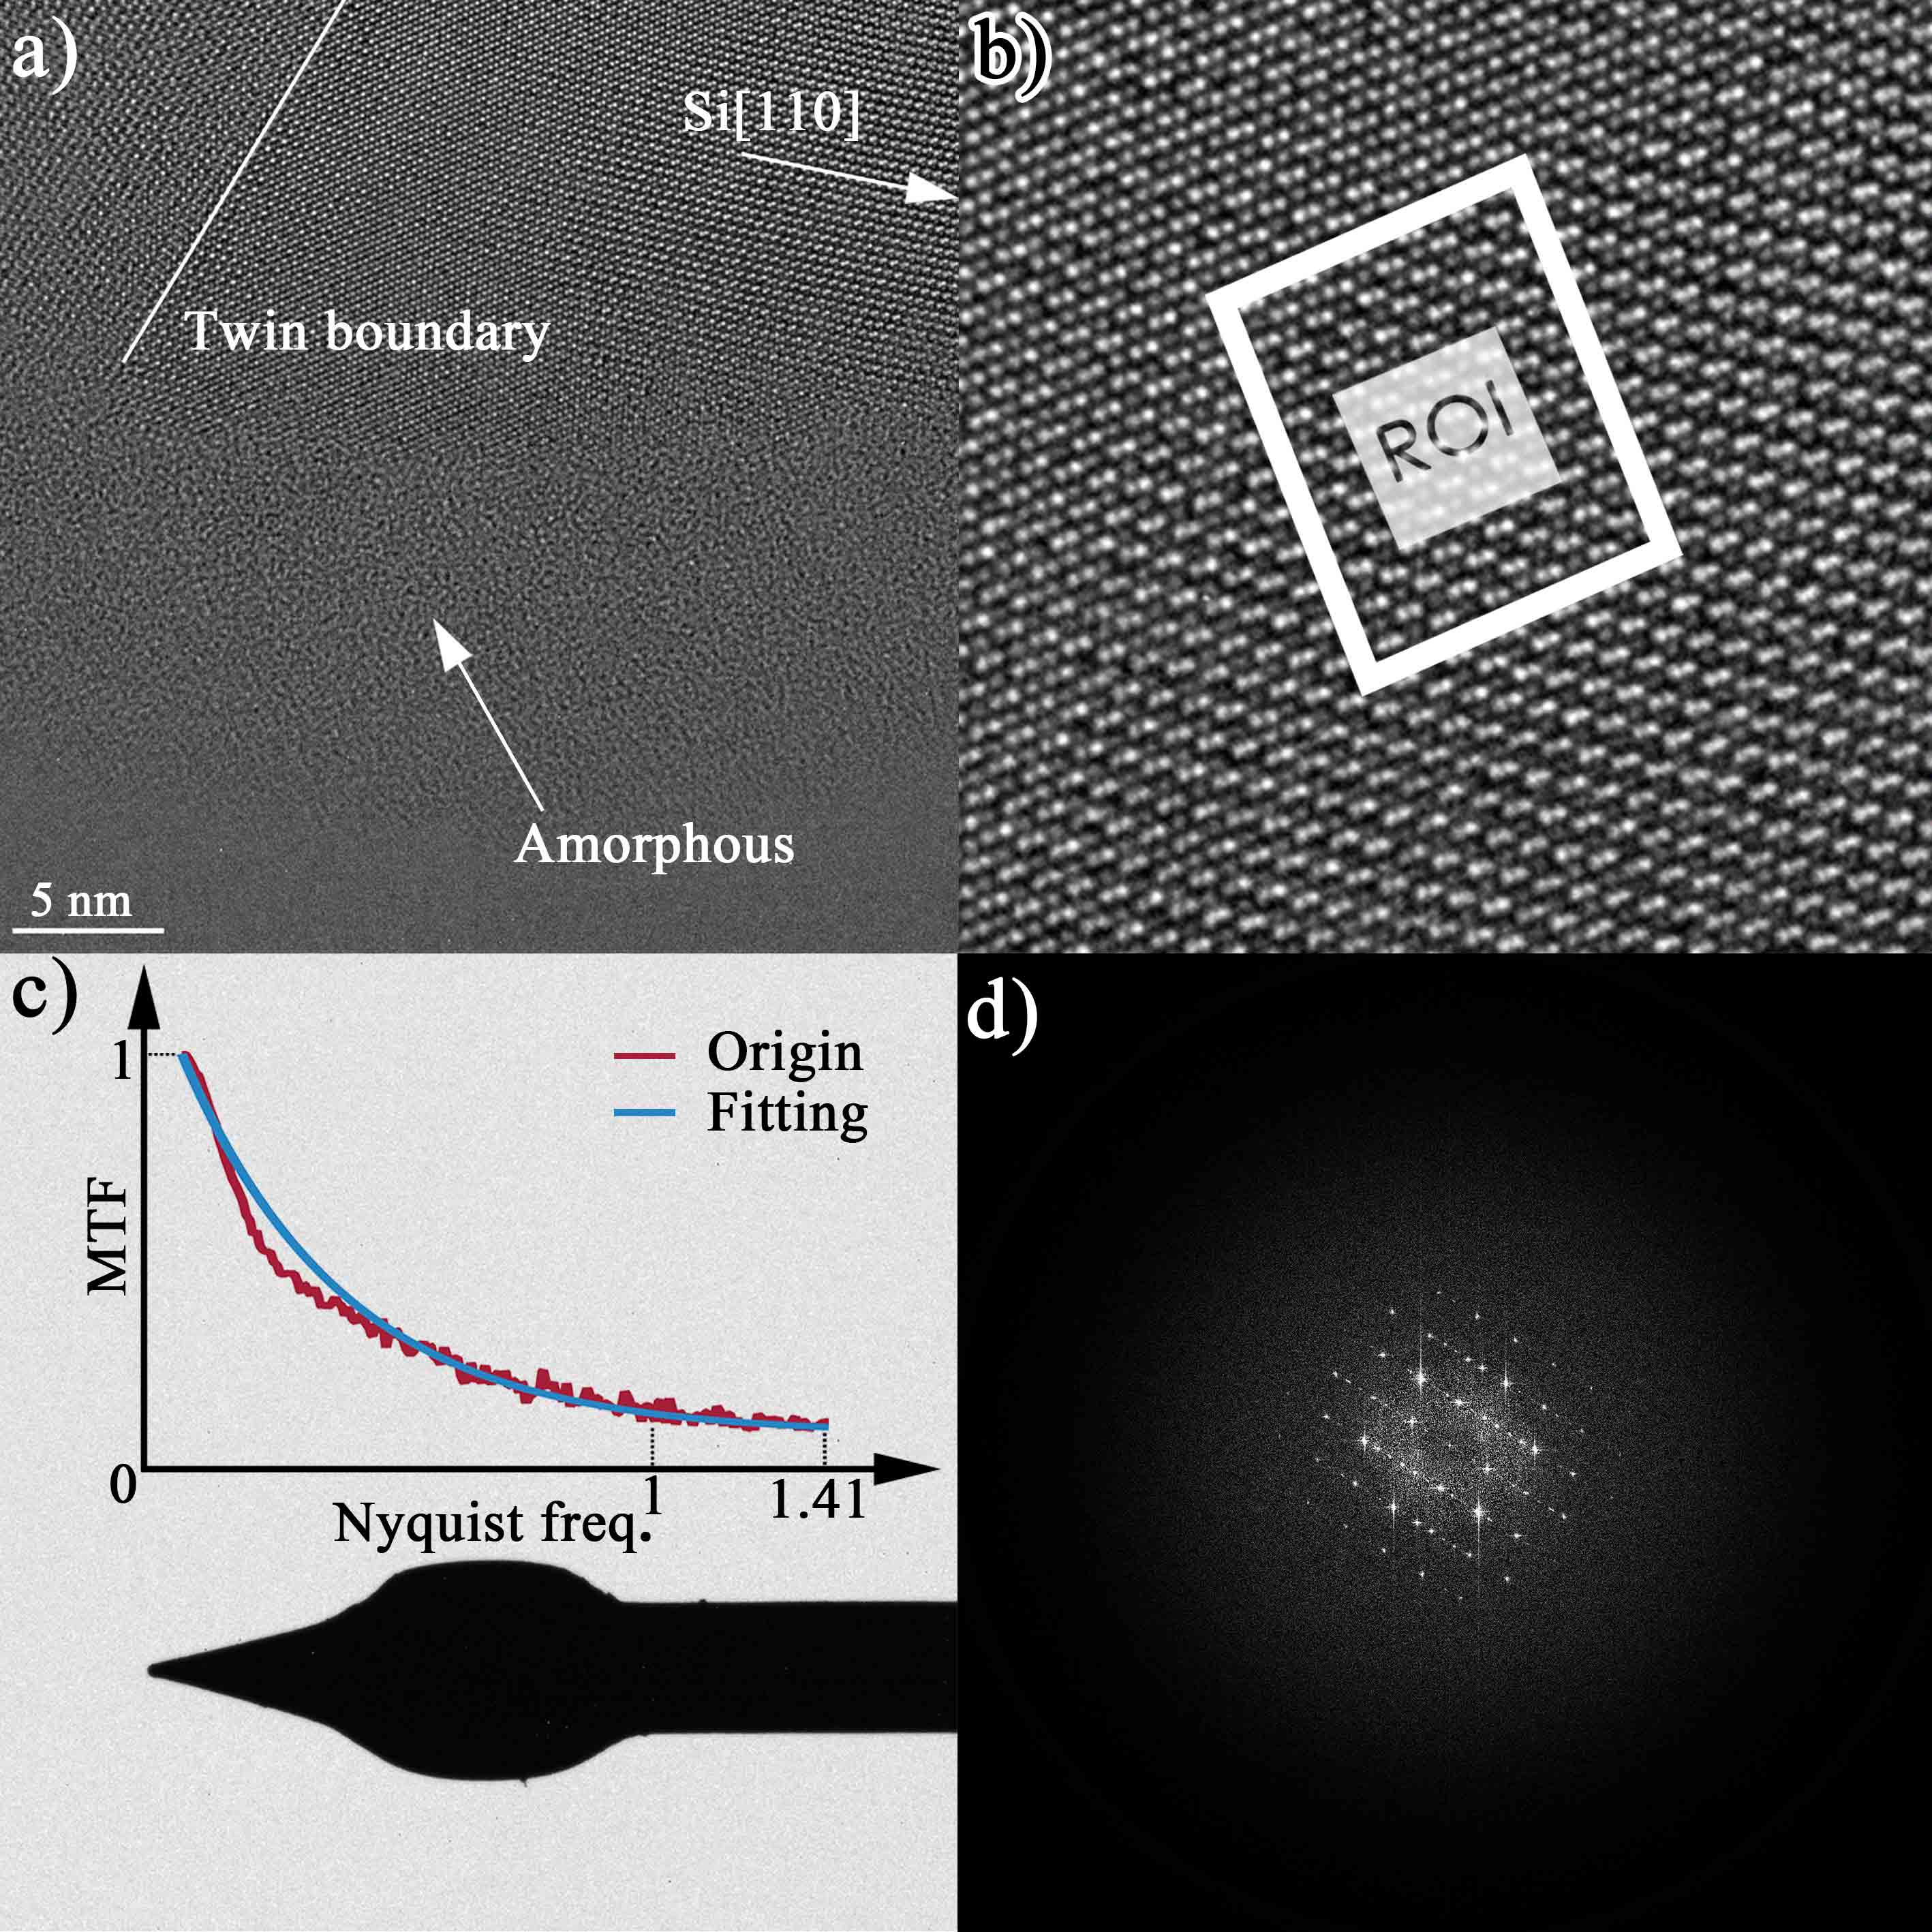
\includegraphics[width=0.85\textwidth]{../2.13/213}
	\caption{实验图像及其预处理}\label{fig:213}
	\song\tuzhu{a) 纳米 Si 颗粒的原子分辨率高分辨 TEM 照片;b) 图 a 中 Si[110] 区域的放大图,矩形区域是待重构的部分;c) 通过挡针像测量相机的 MTF,红色曲线是测量所得的 MTF 曲线,蓝色曲线是根据文献$^{[89]}$中的公式(13 )拟合的 MTF 曲线;d) Weiner 滤波后的 TEM 照片的傅里叶变换图}
\end{figure}

\quad

\begin{table}[htbp]
	\caption{高分辨 TEM 实验照片的成像参数}\label{tab:table1}
	\song\tuzhu\centering{其中 Cs$_3$ 表示三级球差,$\boldsymbol{A}_1$ 表示 2 阶像散,$\boldsymbol{A}_2$ 表示 3 阶像散,$\boldsymbol{B}_2$ 表示彗差,$\boldsymbol{A}_3$ 表示 4 阶像散, $\boldsymbol{S}_3$ 表示星差,$\boldsymbol{A}_4$ 表示 5 阶像散\\}
	\vspace{0.5em}\centering\wuhao
	\renewcommand{\multirowsetup}{\centering}
	\begin{tabular}{cccccccc}
		\toprule[1.5pt]
		Voltage & Cs$_3$ & \qquad$\boldsymbol{A}_1$\quad\quad & \qquad$\boldsymbol{A}_2$\quad\quad & \qquad$\boldsymbol{B}_2$\quad\quad & \qquad$\boldsymbol{A}_3$\quad\quad & \qquad$\boldsymbol{S}_3$\quad\quad & \qquad$\boldsymbol{A}_4$\quad\quad \\
		/kV & /mm & \quad/nm & \quad/nm &\quad/nm & \quad/nm & \quad/nm & \quad/$\upmu$m \\
		\midrule[1pt]
		\multirow{2}{1.3cm}{300} & \multirow{2}{1.3cm}{-0.0132} & \quad1.407 & \quad36.42 & \quad18.78 & \quad322.2 & \quad393.1 & \quad45.95\\
		& & \quad9.1$^{\circ}$ & \quad-38.1$^{\circ}$ & \quad-88.4$^{\circ}$ & \quad-19.1$^{\circ}$ &\quad-19.5$^{\circ}$ & \quad-11.6$^{\circ}$ \\
		\bottomrule[1.5pt]
	\end{tabular}
	\vspace{\baselineskip}
\end{table}

\subsection{图像预处理}
在进行定量分析之前,需要对实验图像进行预处理。首先需要排除 CCD 的 MTF 对实际图像强度的影响。在本研究中,MTF 是通过广泛使用的 knife-edge 方法~\cite{Thust2009}测量得到的。如图 4.14c 所示,这个方法使用电镜中的挡针锋锐的边界来测量 MTF。测量之后的 MTF 数据将根据拟合方法~\cite{VanBroek2012}进行计算得到拟合的 MTF 曲线,如图 4.14c 中蓝色曲线所示。之后将实验图像的傅里叶变换除以 MTF 以去除 MTF 对图像衬度的影响。图 4.15a 和 b 分别展示了原始实验图像和 MTF 矫正之后的图像,MTF 矫正后的图像的衬度略微提升。接着使用了 Weiner 滤波器降低图像中的噪音,降噪后的图像的傅里叶变换如图 4.14d 所示,降噪后的实验图像如图 4.15c 所示。最后将实验图像的图像强度归一化,否则无法与模拟像进行定量对比。归一化的方法是将实验图像的图像强度除以真空部位的平均图像强度~\cite{Hytch1994}。

\begin{figure}[htbp]
	\vspace{\baselineskip}
	\centering
	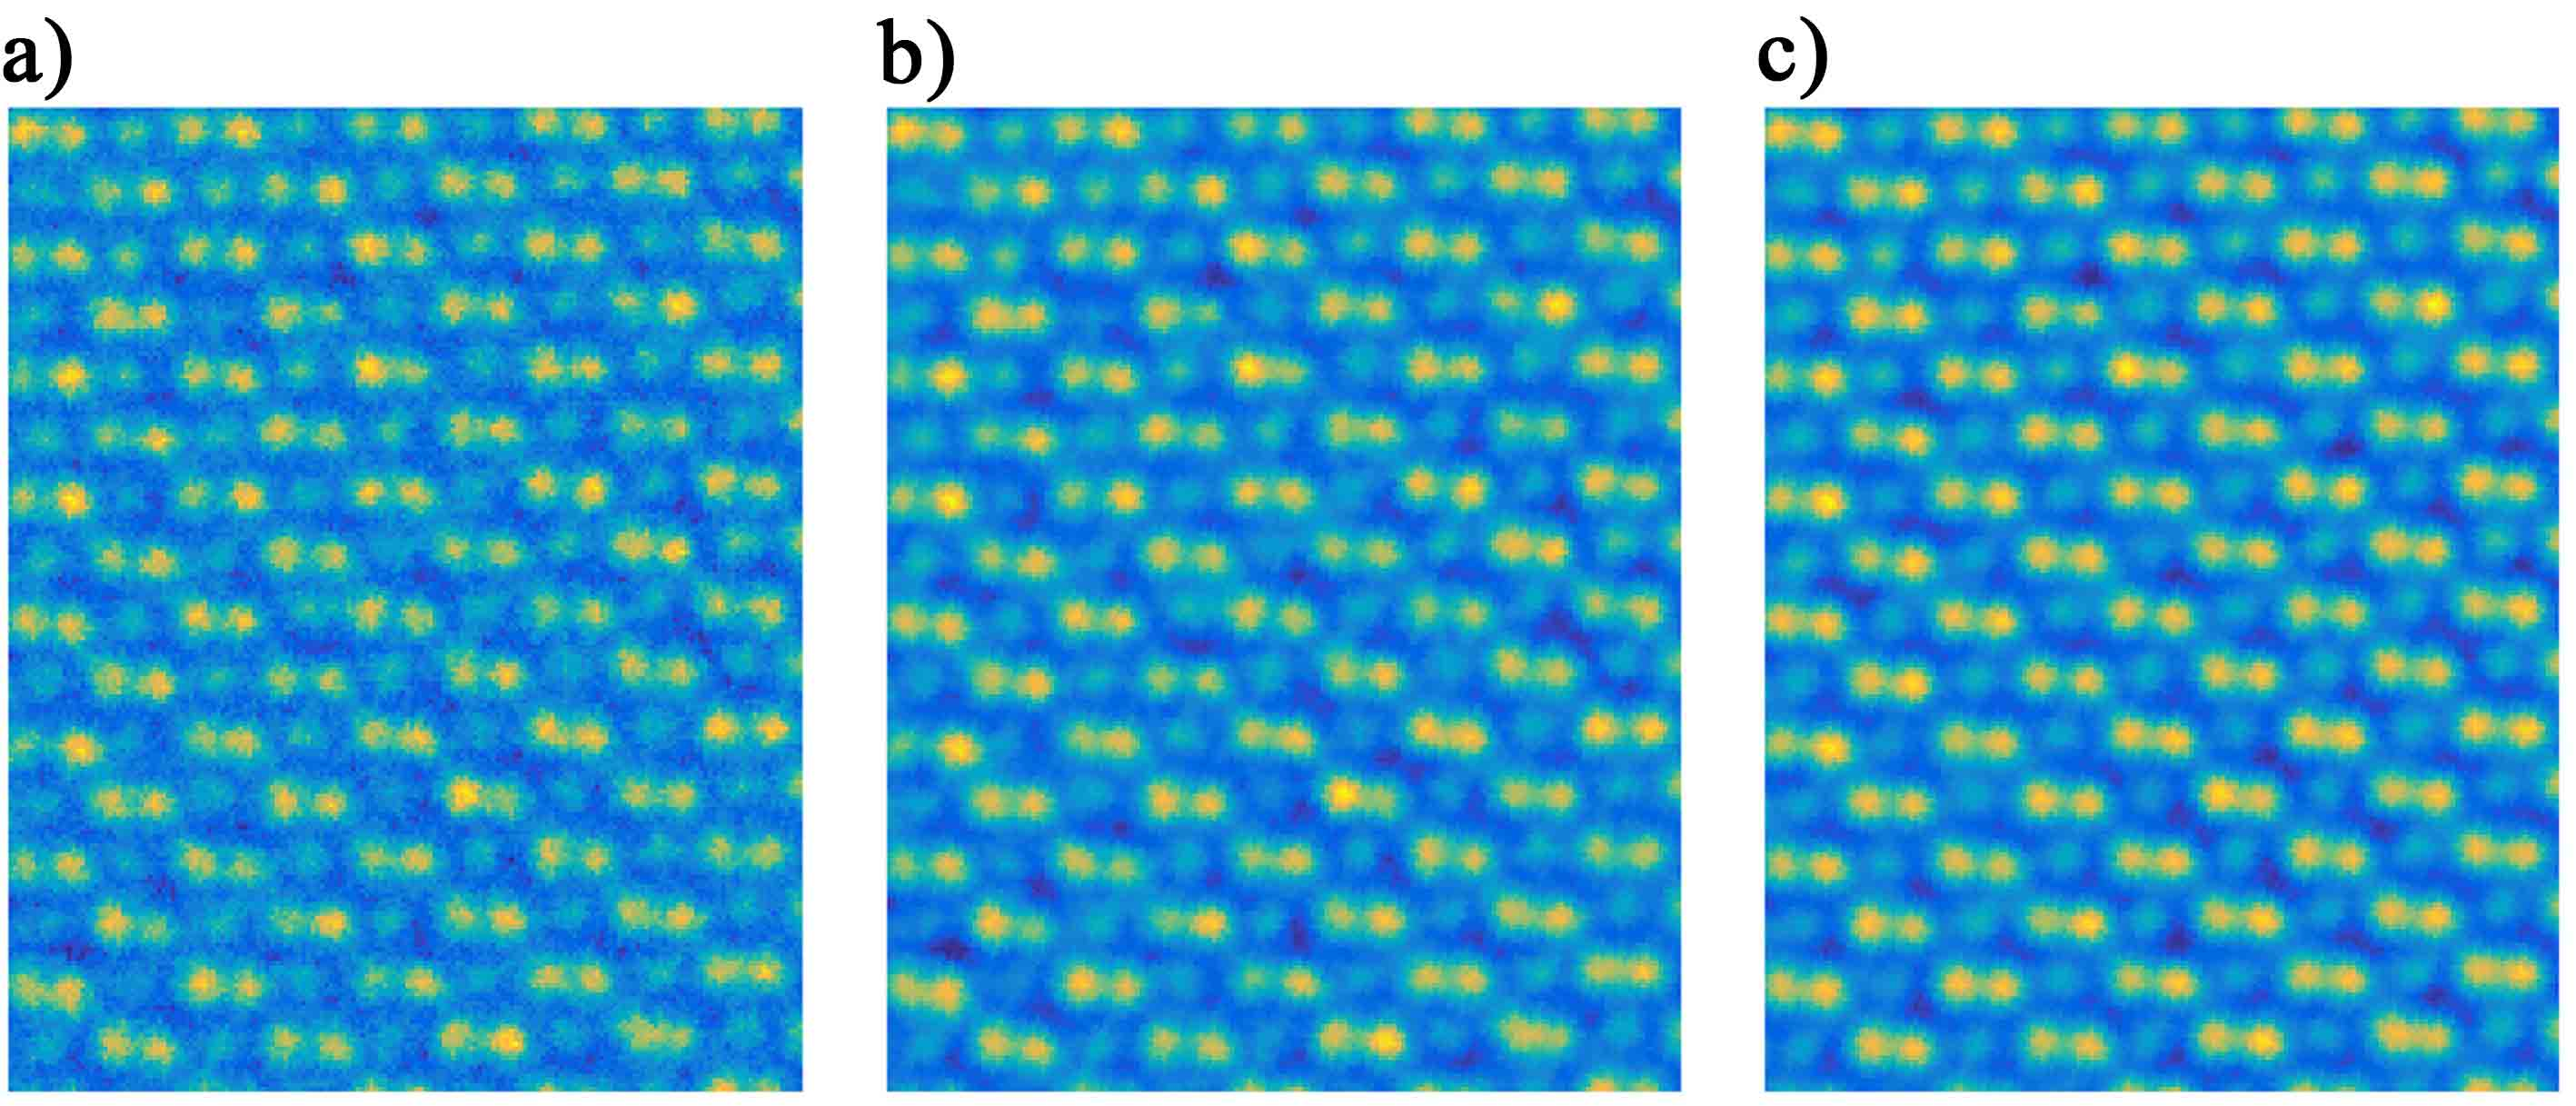
\includegraphics[width=0.9\textwidth]{../2.14/214}
	\caption{图像预处理过程中的图像变化}\label{fig:214}
	\song\tuzhu{a) 原始实验图像;b) MTF 矫正后的实验图像;c) 最后经过 Weiner 滤波后的图像}
\end{figure}

\subsection{三维重构过程}
为了定量对比实验像与模拟像的图像强度,必须选择正确的参数进行图像模拟。在本研究中,根据 H.X. Gao 等的研究~\cite{Gao1999},Si 原子的德拜沃勒因子取值为 $\rm{0.52\ \mathring{A}^2}$。且经过探究可知德拜沃勒因子的微弱变动对重构结果没有明显的影响。通过仔细的分析,在所选的待重构区域并没有观察到明显的晶体倾转。成像时的像差参数可参考表 4.3,由于实验时使用了球差矫正器,所以这些像差数值都非常小。由于样品中存在原子的弛豫和残余应力,实际 TEM 样品中的原子并不完全按照理想的 Si 晶体中的原子位置排列,所以每一个 Si 原子柱的位置都需要被精准地测量,并且反复对比实验像与模拟像以确定各原子柱的位置。图 4.16b 展示了测量的 Si 原子柱位置与理想的 Si 原子柱位置的对比图。




\begin{figure}[H]
	\vspace{\baselineskip}
	\centering
	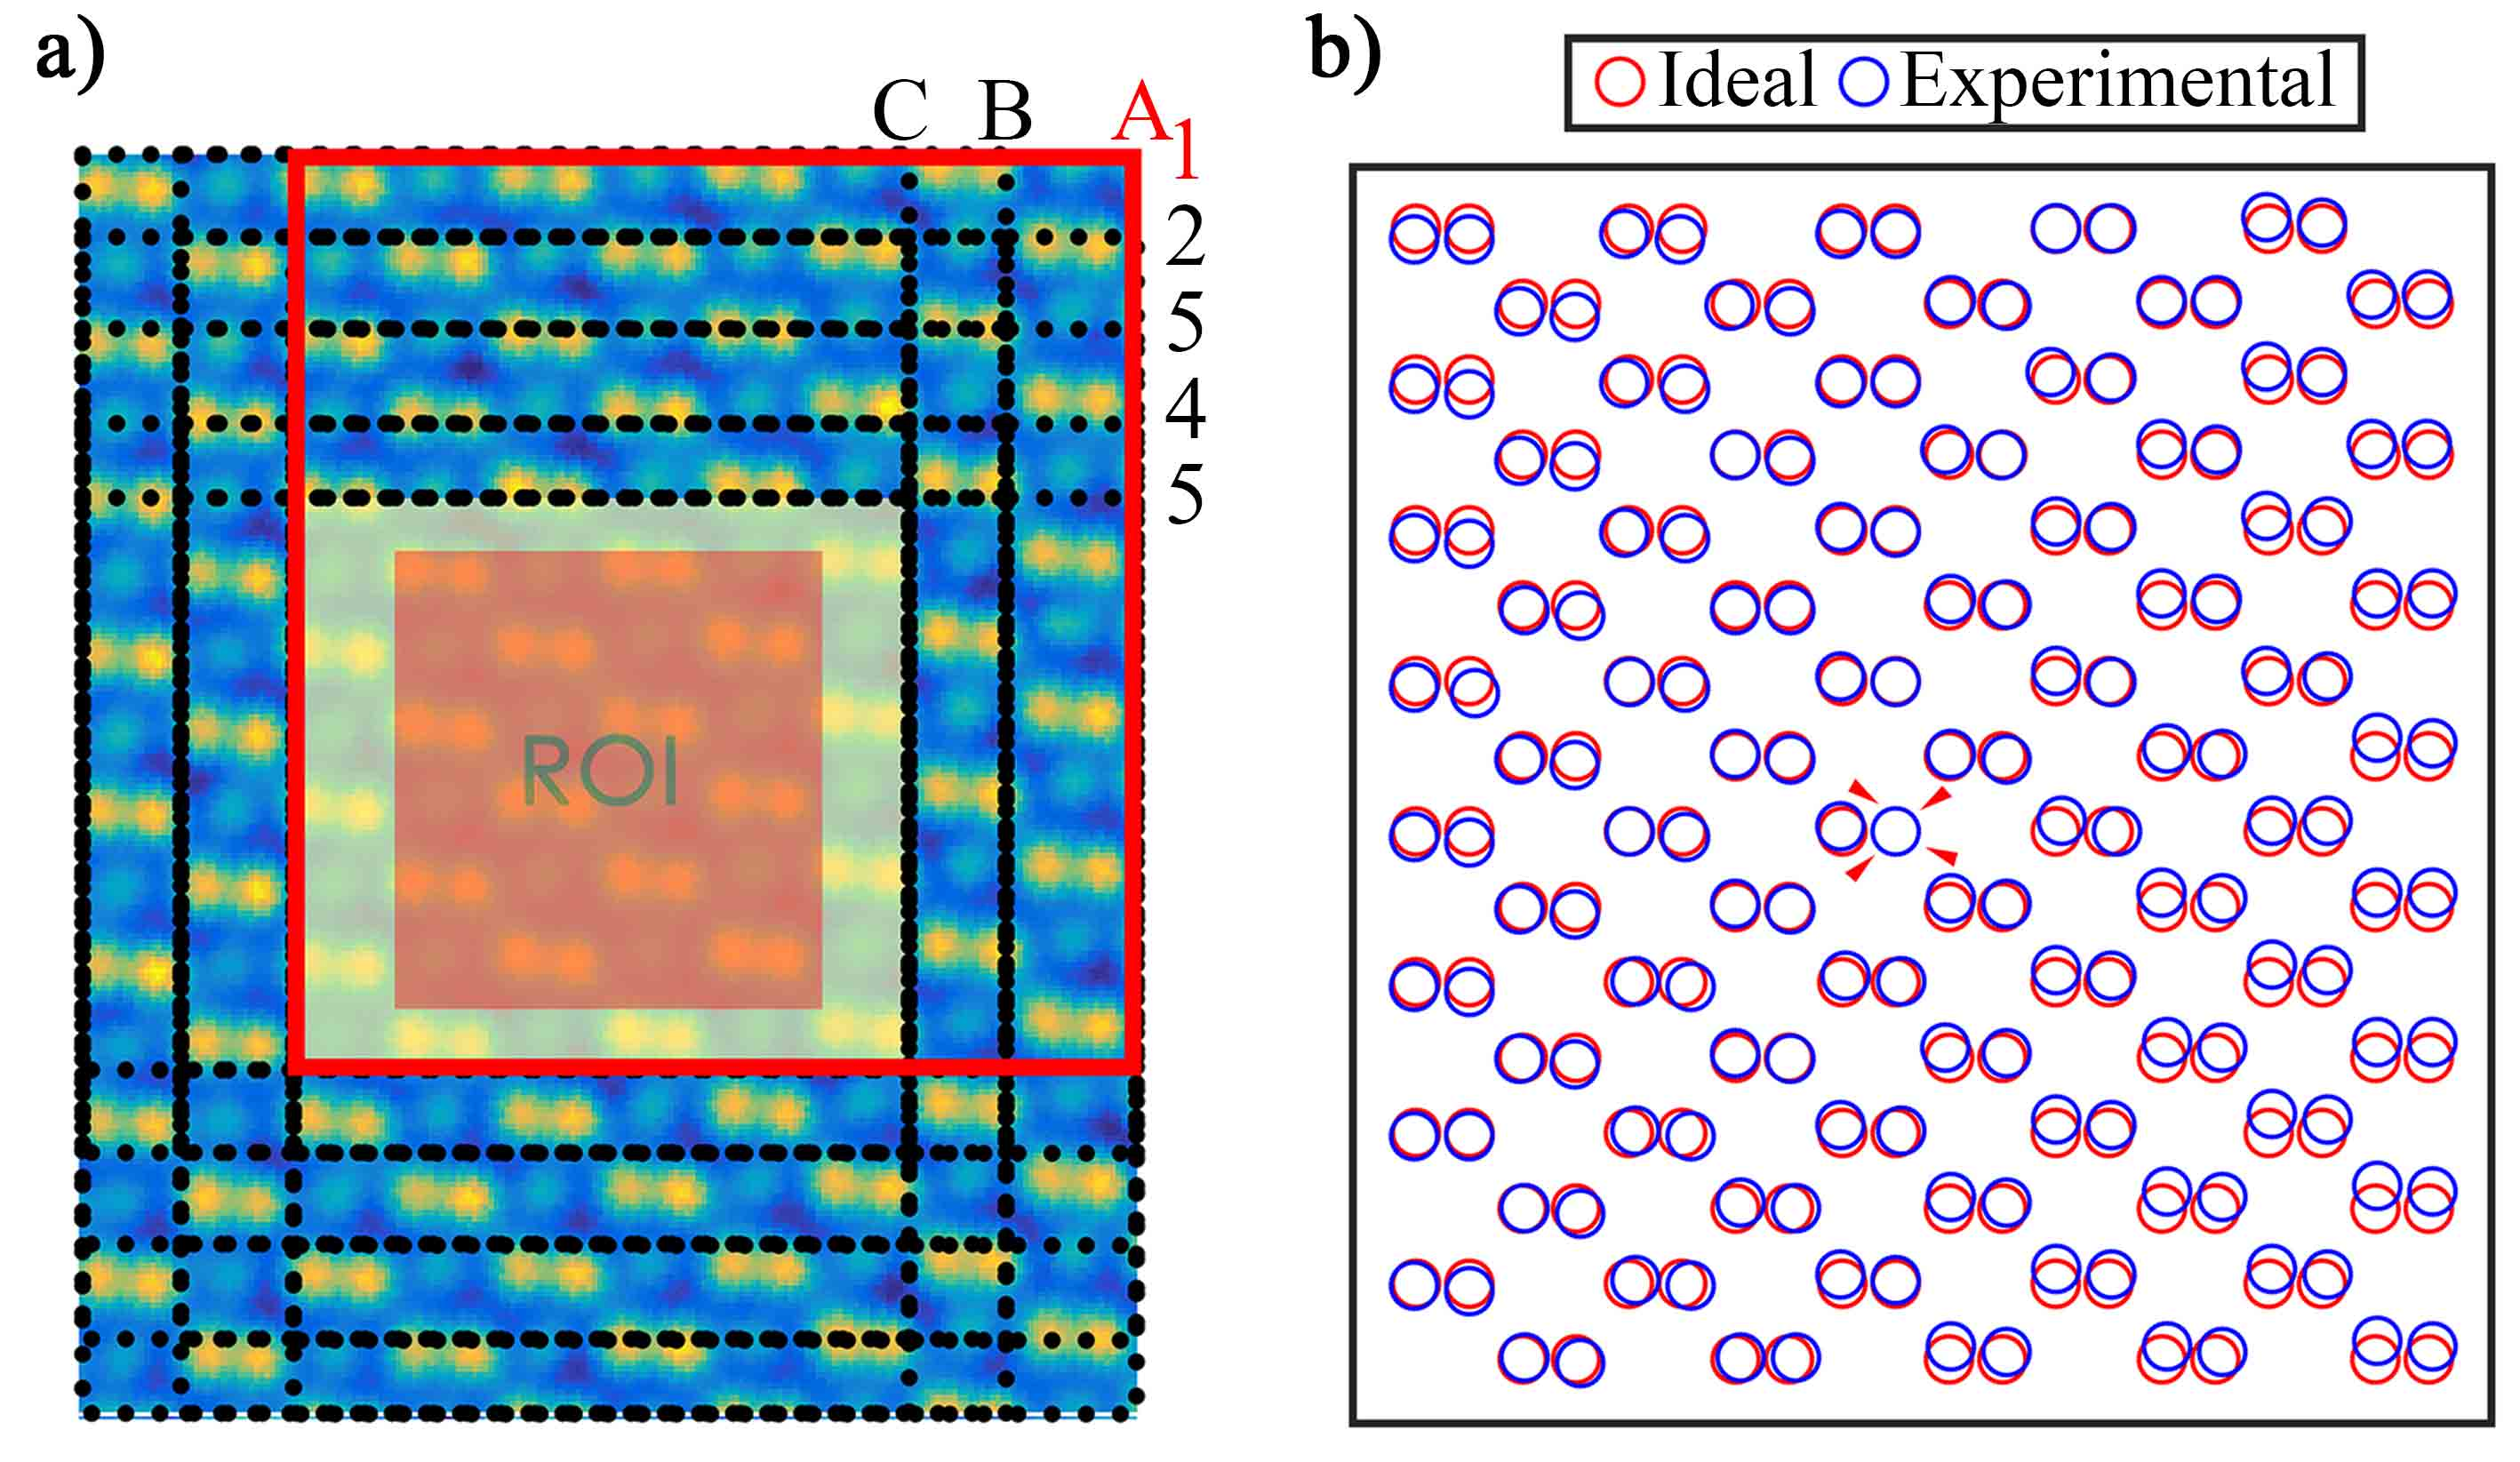
\includegraphics[width=0.9\textwidth]{../2.15/215}
	\caption{重构区域的划分以及 Si 原子柱位置的测量}\label{fig:215}
	\song\tuzhu{a) 待重构的实验图像,图中红色部分是感兴趣区域,A1,A2,…,C5 分别是 15 个相同尺寸的超胞,黄色区域是它们的公共区域,这些超胞将用于 15 次独立的重构;b) 理想晶体中的 Si 原子柱位置和实际测量的 Si 原子柱位置,中间红色箭头标记的是这两套原子柱位置的重合处}
\end{figure}

如第 4.3.2 条中所述,为了得到可靠的重构结果,需要采取自洽性验证方案,对同一个感兴趣区域进行多次独立的三维重构,最后通过统计数据定量分析三维重构的分辨率,以及得到最终的重构结果的置信度。在本次实验图像的重构中,如图 4.16a 所示,共选取了 15 个相同尺寸的单胞来重构中间的感兴趣区域。图 4.17a 展示了某三次重构的重构结果的上表面示意图,图 4.17b 展示了相应的下表示意图。观察可知,这几次重构的重构结果非常接近,但总是存在略微不同。图 4.17c 展示了重构的感兴趣区域的平均结果中每一个原子柱的厚度和高度。

为了估算三维重构 $z$ 方向上的分辨率,图 4.18a 和 b 统计了每一个 Si 原子柱的厚度以及高度的重构结果。其中橙色标记了各原子柱的平均结果。表 4.4 展示了 15 次独立重构各自的最大绝对误差。根据以上数据可知,全局匹配算法的稳定性很高,15 次重构的重构结果之间的差异很小。在原子柱厚度方面, 15 次重构结果的最大误差都是 1 个原子间距(0.384 nm);在原子柱高度方面,有 13 次(86.7\%)重构的最大误差是 1 个原子间距,其他 2 次(13.3\%)重构结果的最大误差是 2 个原子间距。因此,根据上文中提出的定义三维重构分辨率的原则,扣除前 20\% 的大误差,本次重构的分辨率在原子柱厚度和高度上均是 1 个原子间距,这意味着 Si 样品的表面形貌在原子分辨率下被重构了出来。

\quad

\begin{figure}[H]
	\vspace{\baselineskip}
	\centering
	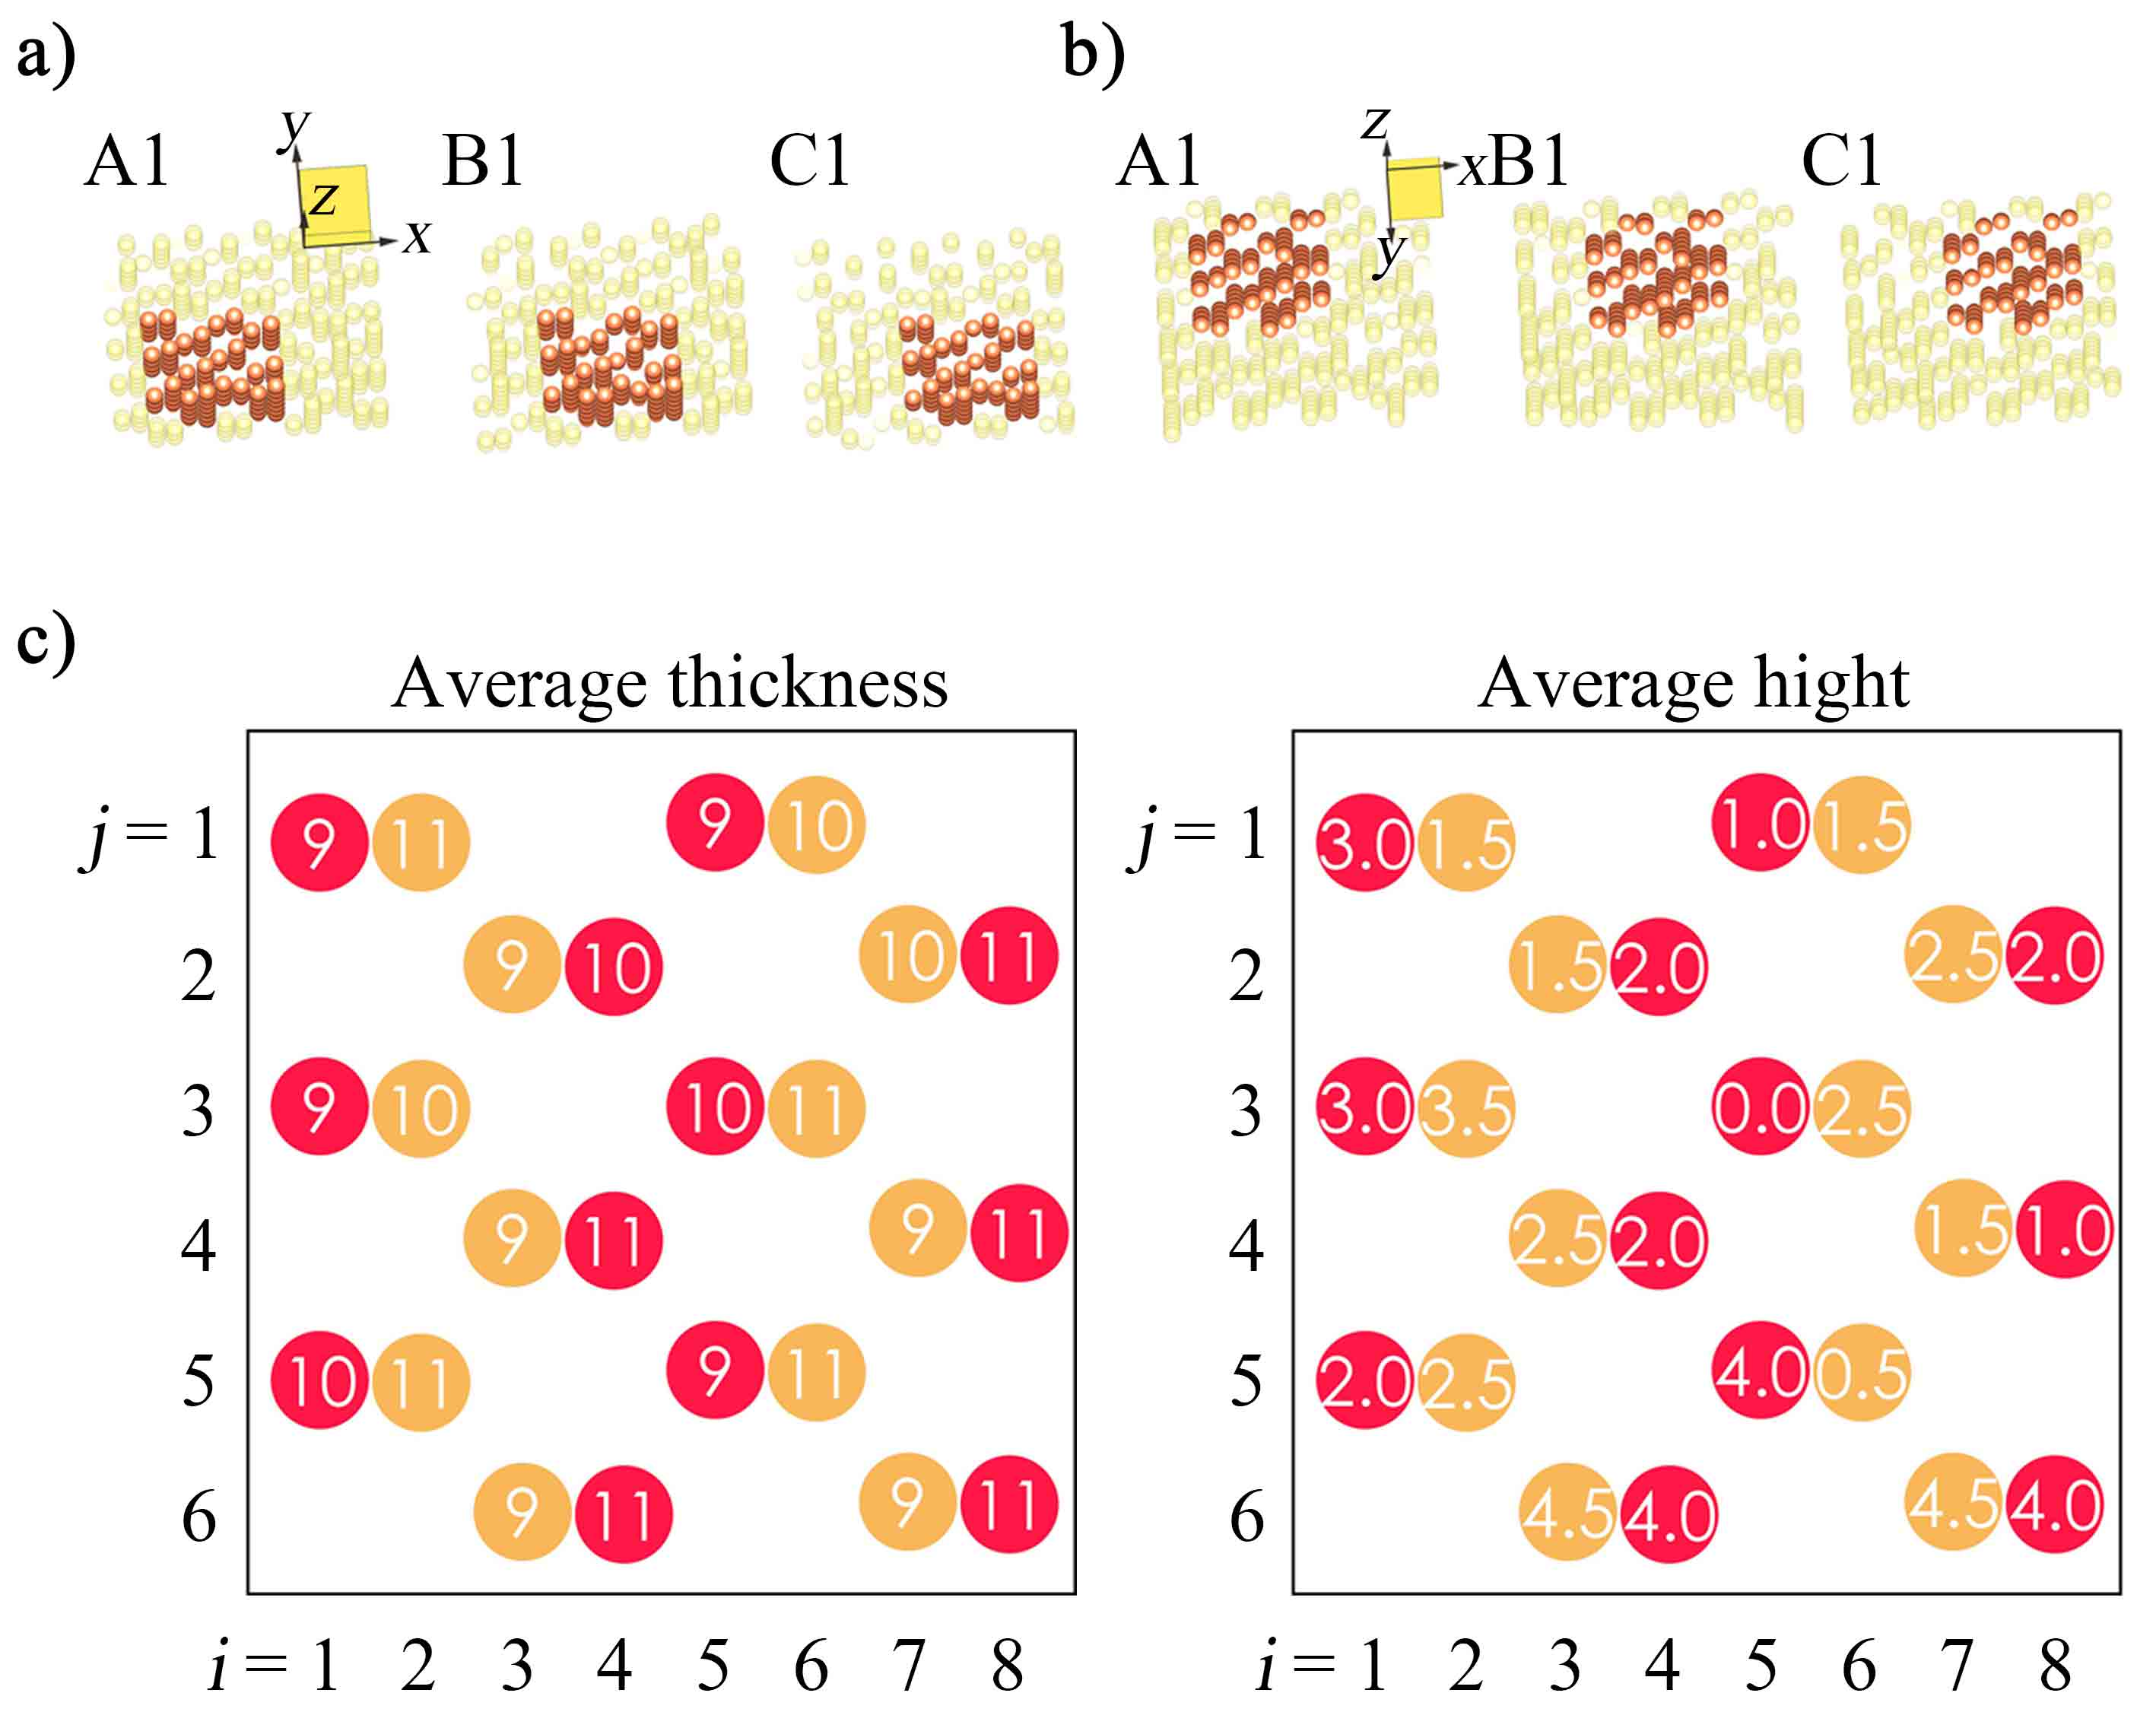
\includegraphics[width=0.9\textwidth]{../2.16/216}
	\caption{重构结果示意图}\label{fig:216}
	\song\tuzhu{a) 超胞 A1,B1,C1 的重构结果的上表面示意图;b) 超胞 A1,B1,C1 的重构结果的下表面示意图;图 a 和 b 中,棕色原子表示感兴趣区域内的原子,黄色原子表示其他的原子;c) 感兴趣区域的平均重构结果中每个原子柱的厚度和高度的示意图,单位是原子间距(0.384 nm),红色和黄色的原子柱分别表示原子位置处于单胞中的  0和 0.5c 高度位置}
\end{figure}

\quad

\quad

\quad

\begin{table}[H]
	\caption{15 次独立重构结果中原子柱厚度与高度的最大绝对误差,单位为一个原子间距(0.384 nm)}\label{tab:table1}	
	\vspace{0.5em}\centering\wuhao
	\begin{tabular}{c!{\vrule width 1pt}ccccccccccccccc}
		\toprule[1.5pt]
		\diagbox[linewidth=1pt]{Para.}{Cell} & A1 & A2 & A3 & A4 & A5 & B1 & B2 & B3 & B4 & B5 & C1 & C2 & C3 & C4 & C5 \\
		\midrule[1pt]
		Thickness & 1 & 1 & 1 & 1 & 1 & 1 & 1 & 1 &1 & 1 & 1 &1 &1 &1 & 1\\
		Height & 1 & 1 & 1 & 1 & 1 & 1 & 1 & 2 &1 & 1 & 1 &1 &2 &1 & 1\\
		\bottomrule[1.5pt]
	\end{tabular}
	\vspace{\baselineskip}
\end{table}


\begin{figure}[H]
	\vspace{\baselineskip}
	\centering
	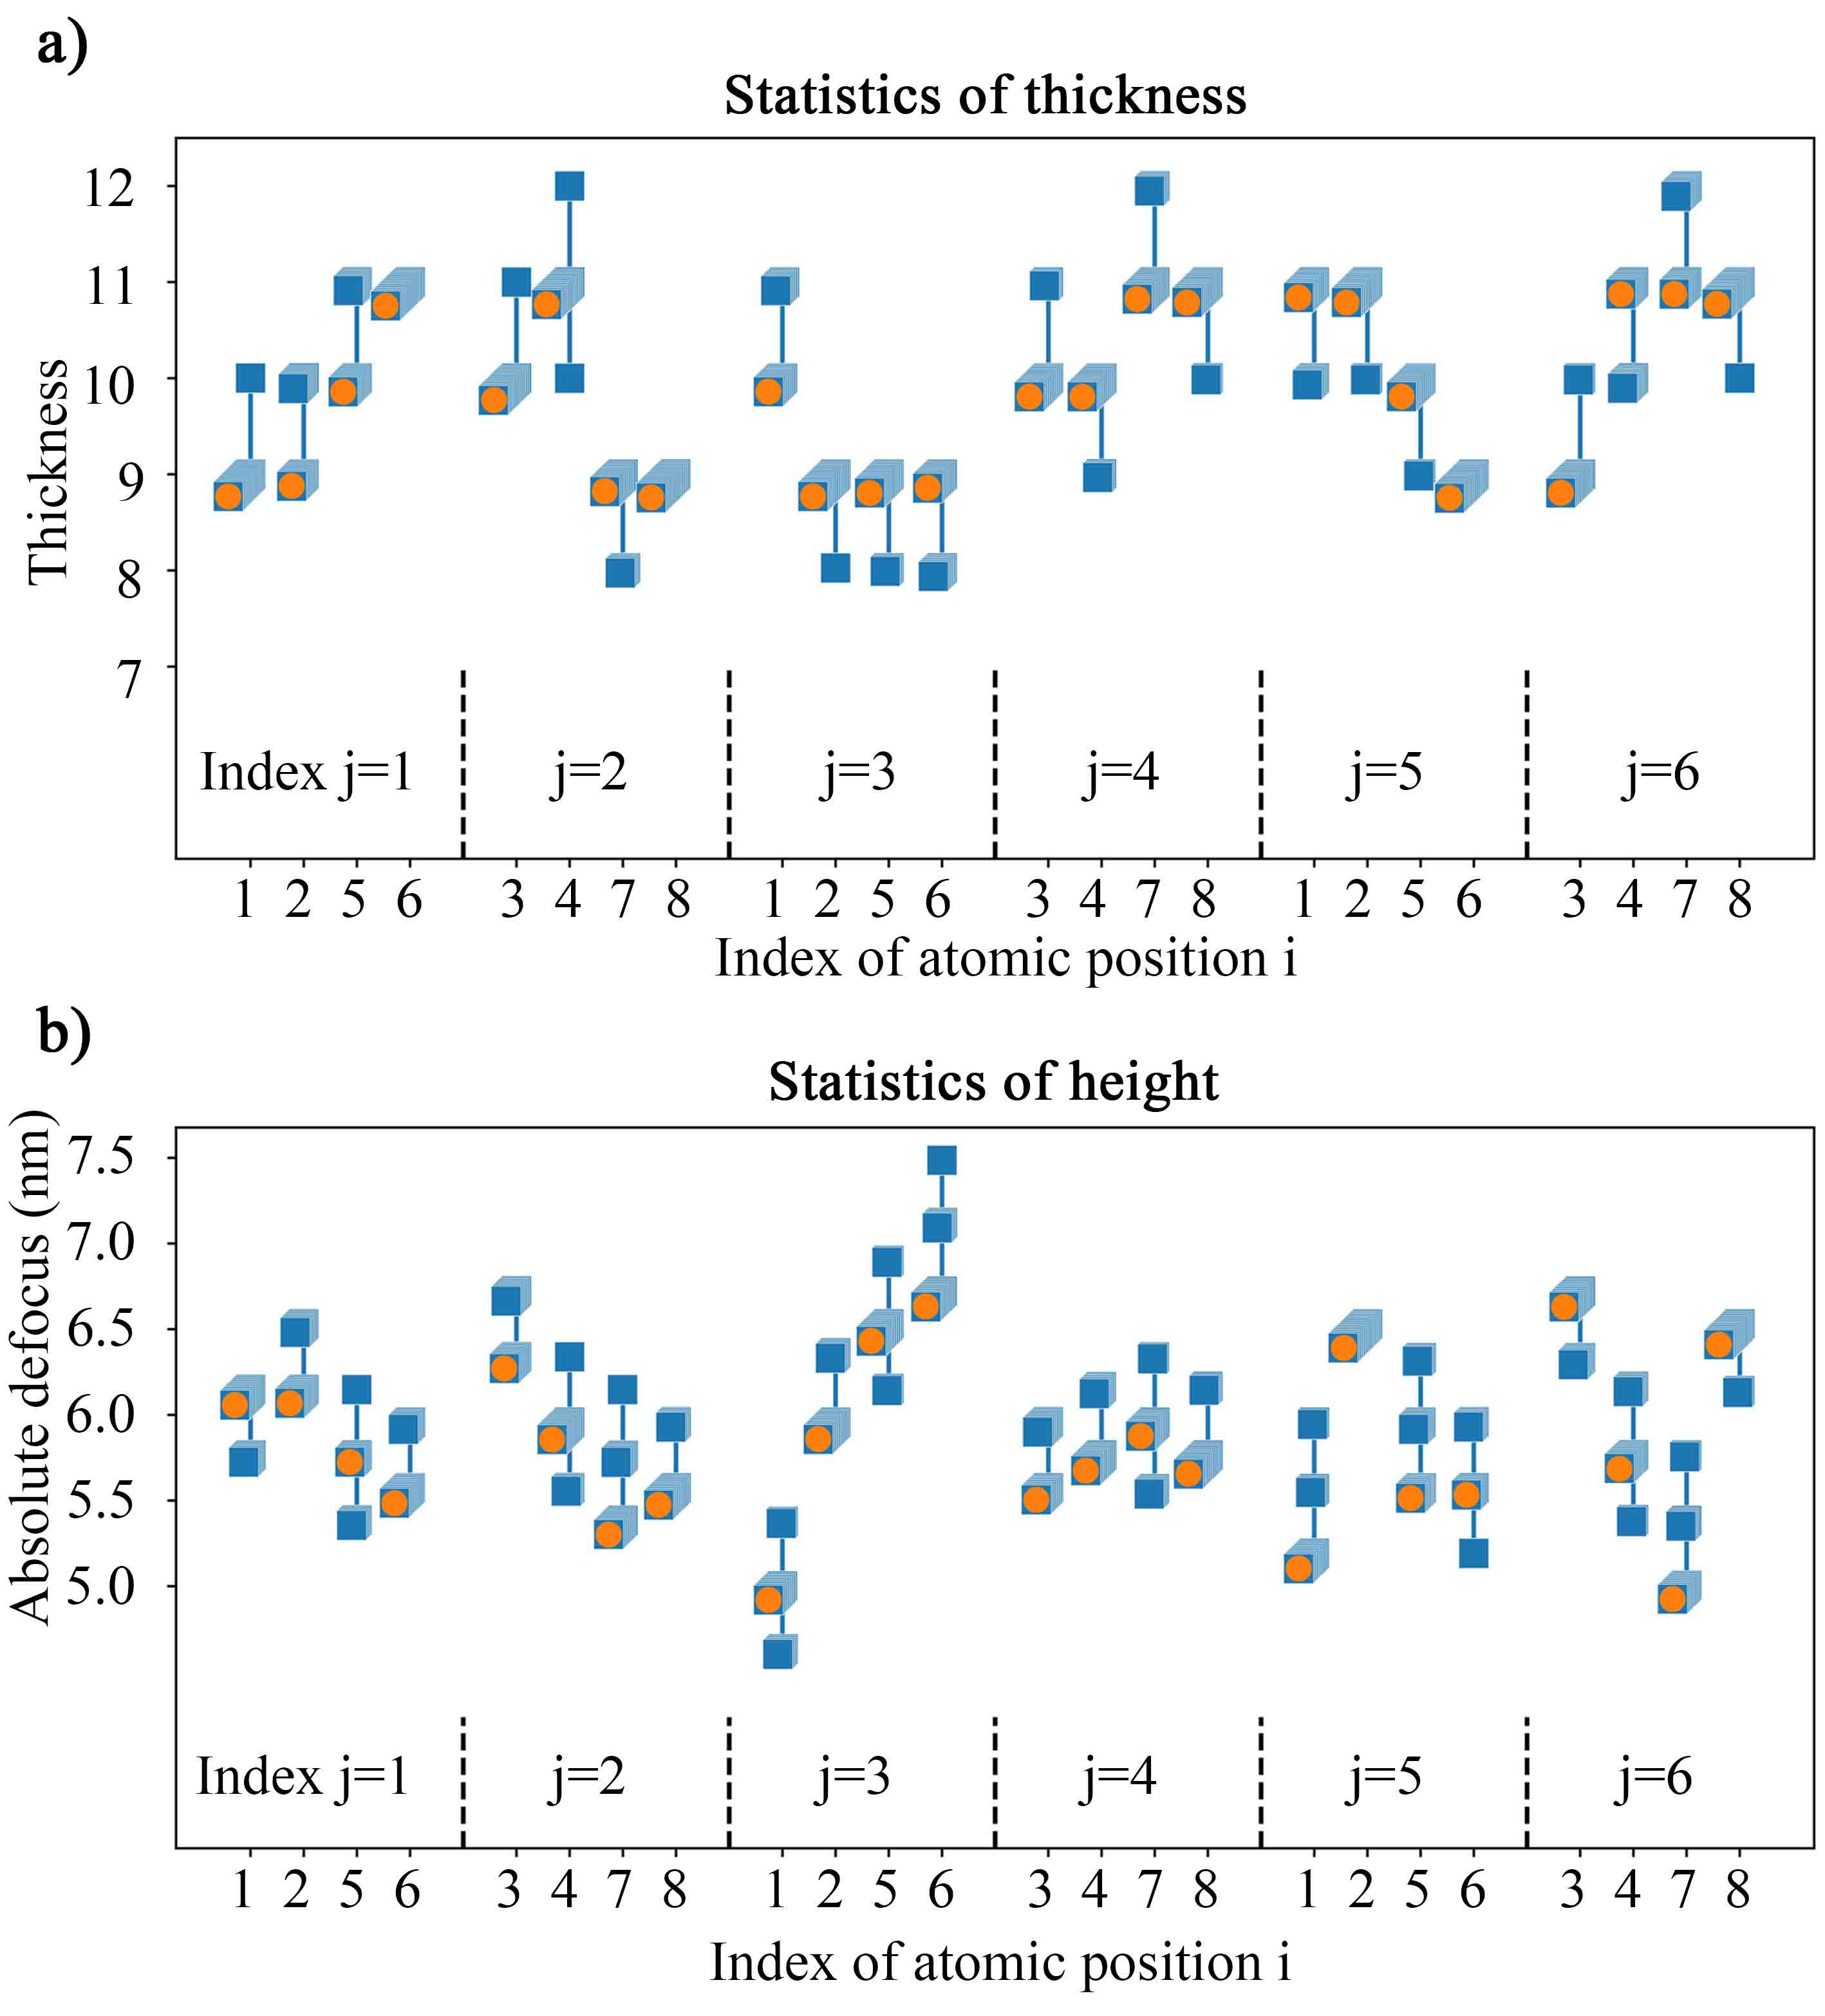
\includegraphics[width=0.85\textwidth]{../2.17/217}
	\caption{各原子柱的重构结果统计}\label{fig:217}
	\song\tuzhu{a) 原子柱厚度的统计结果;b) 原子柱高度的统计结果;橙色标记的是最终的平均结果,原子柱的索引与图 4.16c 一致}
\end{figure}




为了估算此次 Si[110] 样品的三维重构的置信度,图 4.19a-c 
展示了最终重构结果的高分辨模拟像(图 2.18a),感兴趣区域的实验图像(图 2.18b)以及两图像之间的误差(图 4.19c)。图 4.19c 的平均相对误差是 3.76\%,且从中可见,较大的误差发生在原子柱位置之间。进一步对比各原子柱位置的图像强度的结果如图 4.19d和 e 所示。其中,原子柱位置的图像强度是原子柱位置周围 $5\times 5$ 像素的平均强度值。模拟像中的原子柱位置的图像强度与实验像中原子柱位置的图像强度吻合度很高。原子柱位置的平均误差 $E_{column}$ 仅为 0.91\%。所以,根据公式(4.6)可得本次重构的置信度为 95.33\%。尽管许多不可控的因素将导致随机误差,但是非晶污染是主要的误差来源。在此基础上,根据图 4.13 中晶体厚度为 4 nm 时的误差曲线,估算此 Si[110] 样品表面覆盖的非晶层厚度为 0.5 nm。




\begin{figure}[H]
	\vspace{\baselineskip}
	\centering
	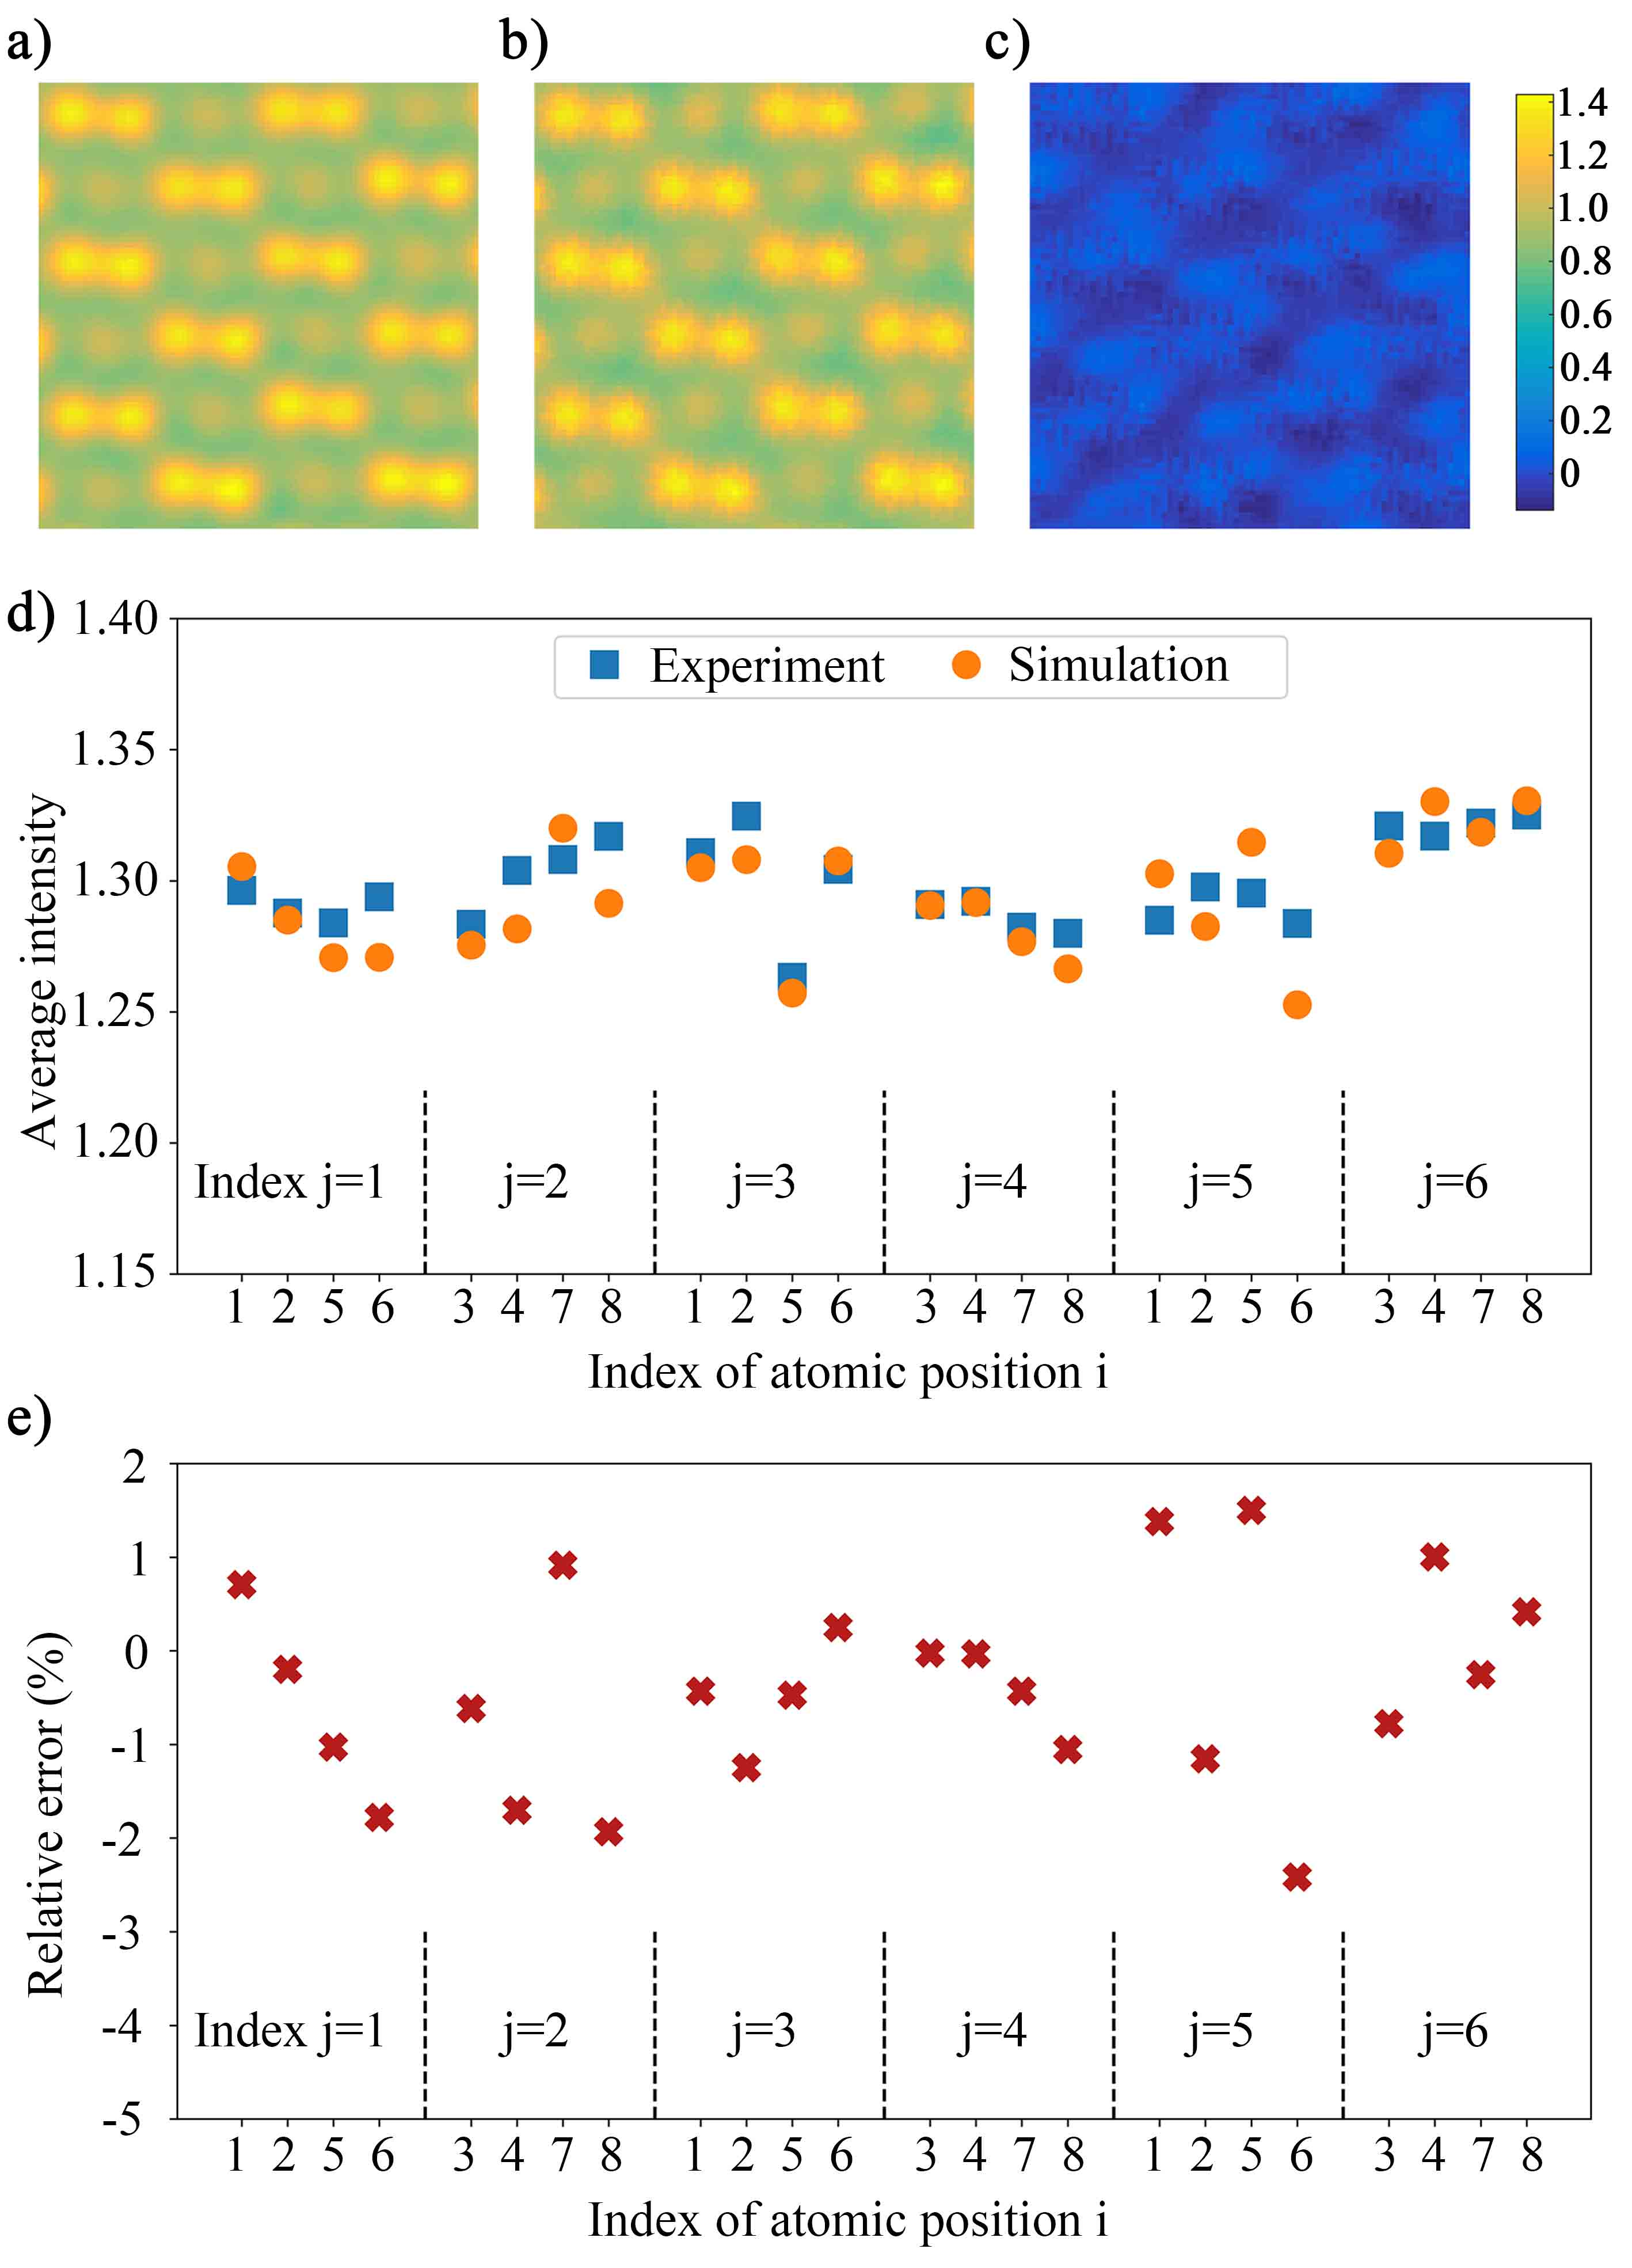
\includegraphics[width=0.85\textwidth]{../2.18/218}
	\caption{重构结果与实验图像的对比}\label{fig:218}
	\song\tuzhu{a) 平均重构结果的模拟像;b) 感兴趣区域的实验像;c) 图 a 和图 b 的差;d)原子柱位置的平均强度的散点图;e)重构的模拟像与实验像原子柱位置图像强度的相比误差;图d)和e)中原子柱的索引与图 4.17c 一致}
\end{figure}


最后,图 4.20a 和 b 展示了平均重构结果的表面原子形貌。图 4.20c 进一步统计了每一个原子柱的厚度(原子个数)和高度(欠焦量),并展示了它们在上表面以及下表面的分布情况。该样品的上下表面不是完全平滑的,而是在原子尺度上存在起伏。尽管不同原子柱的欠焦量不尽相同,但是样品的平均欠焦量为 +5.9 nm(图 4.20c 中下方的黑色虚线所示),这与 NCSI 技术下的最佳成像条件下的欠焦量(根据最佳相位衬度条件~\cite{Urban2009}计算,为 +5.88 nm)非常吻合。另外,样品的平均厚度为 3.84 nm(原子柱中包含 10 个原子)。因为 Si[110] 样品的表面 Si(110) 晶面不是低能量的晶面,所以重构所得样品的晶体表面参差不齐且有非晶覆盖的状态较为合理。而且,在目前的制样方法下,也很有可能产生这种不平整的样品表面状态。


\begin{figure}[H]
	\vspace{\baselineskip}
	\centering
	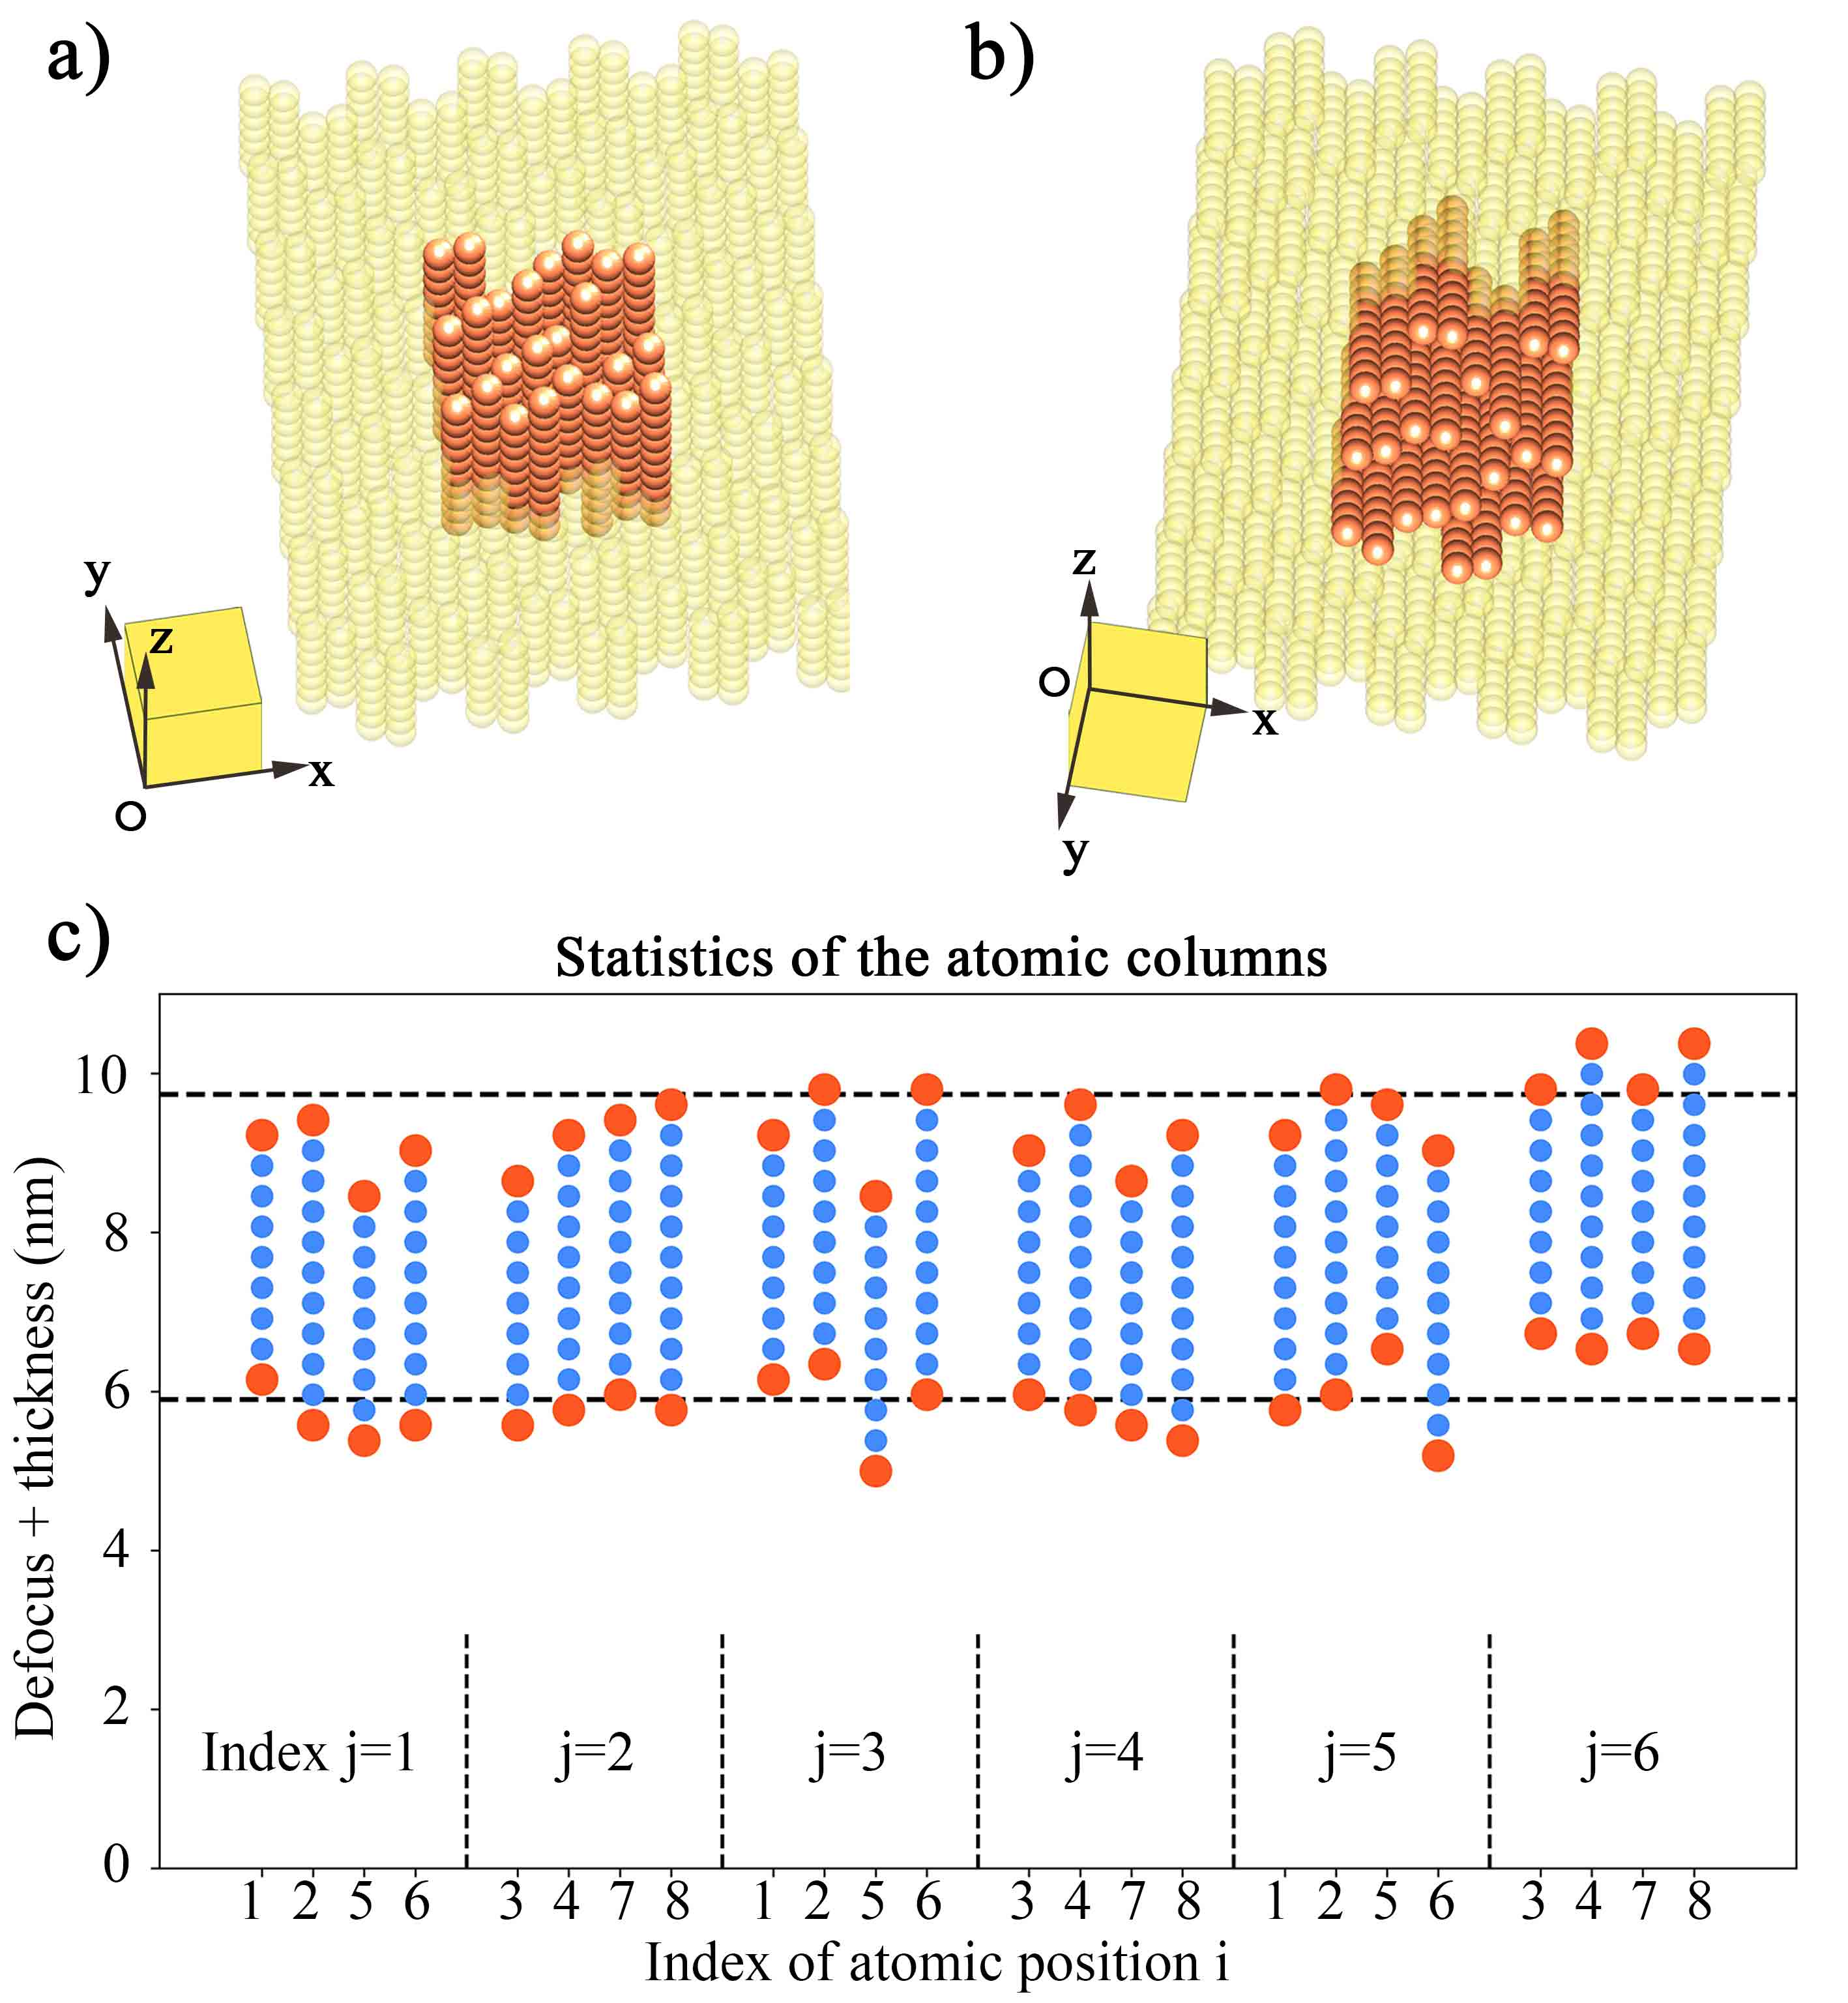
\includegraphics[width=0.8\textwidth]{../2.19/219}
	\caption{重构结果的三维形貌}\label{fig:219}
	\song\tuzhu{a,b) Si[110] 的 15 次重构的平均结果的上表面与下表面的示意图;c) 平均结果中每一个原子的空间绝对位置示意图,其中原子柱的索引与图 4.17c 一致}
\end{figure}






\section{本章小结}
本章提出了一种基于单张二维原子分辨率高分辨 TEM 照片重构材料三维原子形貌的方法。该方法利用了全局匹配算法定量对比实验像与模型像。研究中使用了模拟和实验的图像来测试该方法,从测试结果可以得出以下结论:

(1)为了在原子分辨率下从单张二维图像重构一般的晶体材料的表面,必须采取全局匹配算法和自洽性验证方案。这个方案采取若干次独立的三维重构的平均重构结果作为三维重构的最终结果。三维重构的分辨率可以定义为多次独立重构的重构结果之间的最大误差。同时,高于 90\% 的置信度也是保证三维重构可靠性的一个重要的指标。置信度可以通过定量对比重构结果的模拟像与原始实验图像来确定。


(2)三维重构的分辨率与置信度,与实验图像的质量密切相关。而实验图像的质量往往最容易受非晶污染的影响。如果实际样品表面覆盖的非晶厚度小于 1 nm,则三维重构的结果较可靠。
